%=================================================================
\documentclass[universe,article,submit,moreauthors,pdftex,a4paper]{Definitions/mdpi}
%=================================================================
\firstpage{1} 
\makeatletter 
\setcounter{page}{\@firstpage} 
\makeatother
\pubvolume{xx}
\issuenum{1}
\articlenumber{5}
\pubyear{2020}
\copyrightyear{2020}
%\externaleditor{Academic Editor: Roman Pasechnik}

%\preto{\abstractkeywords}{\nolinenumbers} %>>>>nolinenumbers<<<
%\history{Received: 10 September 2020; Accepted: date; Published: date}
%\updates{yes} % If there is an update available, un-comment this line

%% MDPI internal command: uncomment if new journal that already uses continuous page numbers 
%\continuouspages{yes}

%------------------------------------------------------------------
% The following line should be uncommented if the LaTeX file is uploaded to arXiv.org
\pdfoutput=1

%=================================================================
% Add packages and commands here. The following packages are loaded in our class file: fontenc, inputenc, calc, indentfirst, fancyhdr, graphicx,epstopdf, lastpage, ifthen, lineno, float, amsmath, setspace, enumitem, mathpazo, booktabs, titlesec, etoolbox, tabto, xcolor, soul, multirow, microtype, tikz, totcount, amsthm, hyphenat, natbib, hyperref, footmisc, url, geometry, newfloat, caption
\usepackage{xcolor}
\usepackage{float}
\usepackage{graphicx}
\usepackage{amsmath}
\usepackage{amssymb}
\usepackage{epstopdf}
\usepackage{comment}
\usepackage{draftwatermark}

\newcommand{\TeV}{\text{ TeV}}
\newcommand{\GeV}{\text{ GeV}}
\newcommand{\MeV}{\text{ MeV}}
\newcommand{\keV}{\text{ keV}}
\newcommand{\eV}{\text{ eV}}
\newcommand{\meV}{\text{ meV}}
\newcommand{\beqn}{\begin{equation}}
\newcommand{\eeqn}{\end{equation}}
\newcommand{\req}[1]{Eq.\,(\ref{#1})}
%\newcommand*{\req}[1]{Eq.~{\eqref{#1}}}
\newcommand*{\rf}[1]{Fig.~{\ref{#1}}}
\newcommand*{\rsec}[1]{Sect.\,{\ref{#1}}}
\newcommand*{\bb}{\boldsymbol}
\newcommand*{\xred}{\color{red}}
\newcommand*{\xblue}{\color{blue}}
\newcommand*{\xgreen}{\color{green}}

%=================================================================
%% Please use the following mathematics environments: Theorem, Lemma, Corollary, Proposition, Characterization, Property, Problem, Example, ExamplesandDefinitions, Hypothesis, Remark, Definition, Notation, Assumption
%% For proofs, please use the proof environment (the amsthm package is loaded by the MDPI class).

%=================================================================
% Full title of the paper (Capitalized)
\Title{A SHORT SURVEY OF MATTER-ANTIMATTER EVOLUTION IN THE PRIMORDIAL UNIVERSE}

% Author Orcid ID: enter ID or remove command
\newcommand{\orcidauthorA}{0000-0001-8217-1484} % Add \orcidA{} behind the author's name
\newcommand{\orcidauthorB}{0000-0001-5038-8427} % Add \orcidB{} behind the author's name
\newcommand{\orcidauthorC}{0000-0001-5474-2649} % Add \orcidC{} behind the author's name
\newcommand{\orcidauthorD}{0000-0002-2289-4856}
 
% Authors, for the paper (add full first names)
\Author{Johann Rafelski\orcidA{}, Jeremiah Birrell\orcidD, Andrew Steinmetz\orcidC{}, and Cheng Tao Yang\orcidB{}}
% Authors, for metadata in PDF
\AuthorNames{Johann Rafelski, Jeremiah Birrell, Andrew Steinmetz, and Cheng Tao Yang}

% Affiliations / Addresses (Add [1] after \address if there is only one affiliation.)
\address[1]{%
Department of Physics, The University of Arizona, Tucson, Arizona 85721, USA} 

% Contact information of the corresponding author
\corres{Correspondence: JohannR@arizona.edu}
%; %Tel.: (optional; include country code; if there are multiple corresponding authors, add author initials) +xx-xxxx-xxx-xxxx (F.L.)

% Current address and/or shared authorship
%\firstnote{Current address: Affiliation 3} 
%\secondnote{These authors contributed equally to this work.}
% The commands \thirdnote{} till \eighthnote{} are available for further notes

%\simplesumm{} % Simple summary
%\conference{} % An extended version of a conference paper

% Abstract (Do not insert blank lines, i.e. \\) 
\abstract{In celebration of Remo Ruffini's birthday, his contributions to astrophysics and cosmology and the large number of students he mentored, (see \rf{RemoAtWork}) we offer here a survey of the matter-antimatter evolution of the primordial Universe. While the origin of matter-antimatter asymmetry has remained one of the big questions in modern cosmology today, for much of the Universe's early history, antimatter still played a large role in its evolution. We take the position of the standard model Lambda-CDM Universe without invoking additional novel and unexplored physics. We study and explore the evolution of the Universe implementing the known baryonic asymmetry. We present the composition of the Universe across its temperature history while emphasizing the epochs where antimatter content is essential to our understanding. Special topics will include the creation of matter from quark-gluon plasma (QGP), the free-streaming of the neutrinos, the vanishing of the muons, magnetism in the electron-positron cosmos, and a better understanding of the environment where Big Bang Nucleosynthesis (BBN) occurred producing the light elements. We suggest that the methods used in exploring the early Universe may also provide new insights in the study of exotic stellar cores, magnetars, as well as gamma-ray burst (GRB) events. Further investigation is required in pushing known physics to its extremes in the unique laboratory of the matter-antimatter early Universe.}

\keyword{Particles, Plasmas and Electromagnetic Fields in Cosmology; Quarks to Cosmos;}
%%%%%%%%%%%%%%%%%%%%%%%%%%%%%%%%%%%%%%%
\begin{document}
%%%%%%%%%%%%%%%%%%%%%%%%%%%%%%%%%%%%%%% 

%%%%%%%%%%%%%%%%%%%%%%%%%%%%%%%%%%%%%%%
\begin{figure}[ht]
  \centering  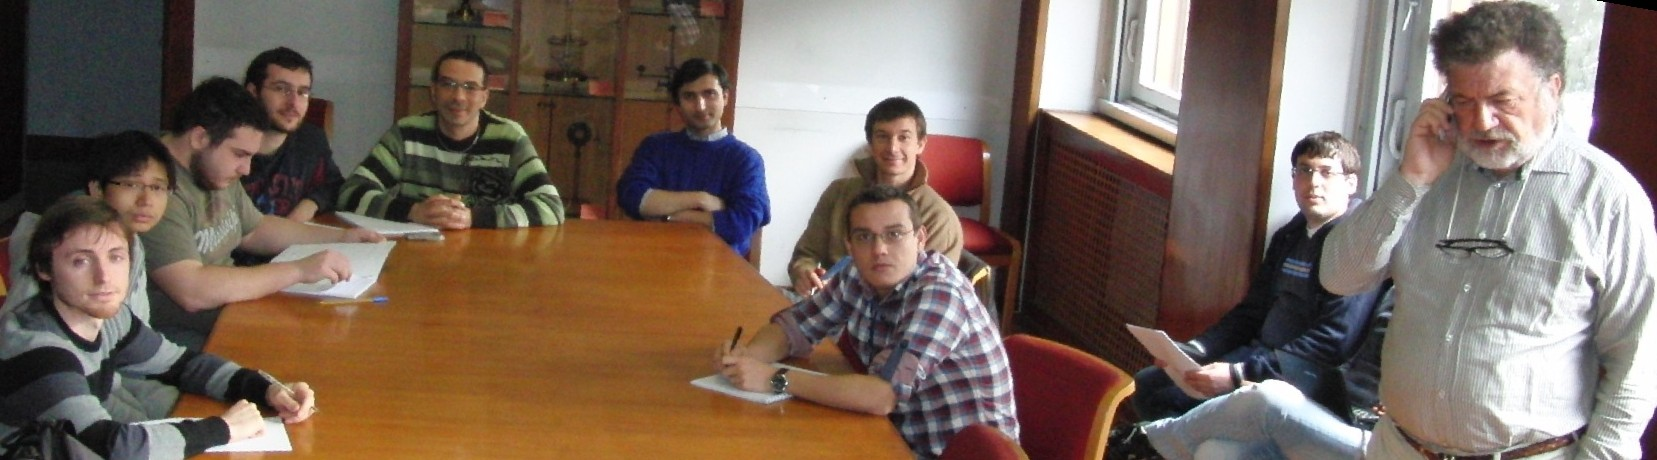
\includegraphics[width=\textwidth]{./plots/12MarchRemoAtWorkC.jpg}
  \caption{\href{https://www.icranet.org/}{ICRANet} group at work, Remo Ruffini on right. Photo by Johann Rafelski. \label{RemoAtWork}}
\end{figure}
%%%%%%%%%%%%%%%%%%%%%%%%%%%%%%%%%%%%%%%

\tableofcontents

\section{Timeline of particles and plasmas in the Universe}\label{sec:Intro}
\subsection{Guide to 130 GeV > T > 20 keV}\label{sec:Guide}
\noindent This survey of the early Universe begins, with elementary particles in their known form today, with quark-gluon plasma (QGP) at a temperature of $T=130\GeV$. It then ends at a temperature of $T=20\keV$ with the electron-positron epoch which was the final phase of the Universe to contain significant quantities of antimatter. This defines the \lq\lq short\rq\rq\ $t\approx1/2$ hour time-span that will be covered. This work presumes that the Universe is homogeneous and that in our casual domain, the Universe's baryon content is matter dominated. We pickup where works like Kolb and Turner \cite{kolb1981early} concluded and coherently connect the differing matter-antimatter plasmas providing background for more specific periods found in the comprehensive literature of observational cosmology \cite{Davis:1985rj,Navarro:1995iw,Moore:1999nt,Springel:2005nw,Demianski:2015xye,Arbey:2021gdg}, the recombination period \cite{Planck:2018vyg,Planck:2018nkj}, BBN \cite{Steigman:2007xt,Cyburt:2015mya,Pitrou:2018cgg}, and baryon asymmetry \cite{Kuzmin:1985mm,Canetti:2012zc,ParticleDataGroup:2022pth} or the origin of dark matter \cite{Bertone:2004pz,Peccei:2006as,Wantz:2009it}. The Universe above temperatures $T>130 \GeV$, involving inflation \cite{Baumann:2009ds,Allahverdi:2020bys} and spontaneous symmetry breaking, is outside the purview of this work.

A more detailed description of particles and plasmas follows in \rsec{sec:Timeline}. We have adopted the standard $\Lambda$-CDM model of a cosmological constant ($\Lambda$) and cold dark matter (CDM) where the Universe undergoes dynamical expansion as described in the Friedmann–Lemaître–Robertson–Walker (FLRW) metric. The contemporary and recent history of the Universe in terms of energy density as a function of time and temperature is shown in \rf{CosmicDensity}. The Universe's past is obtained from integrating backwards the proposed modern composition of the Universe which contains $69\%$ dark energy, $26\%$ dark matter, $5\%$ baryons, and $<1\%$ photons and neutrinos in terms of energy density. The method used to obtain these results are found in \rsec{sec:Cosmo}.

After the general overview, we take the opportunity to enlarge in some detail our more recent work in special topics. In \rsec{sec:QGP}, we describe the chemical potentials of the QGP plasma species leading up to hadronization, Hubble expansion of the QGP plasma, and the abundances of heavy quarks. In \rsec{sec:Hadrons} we discuss the formation of matter during hadronization, the role of strangeness, and the unique circumstances which led to pions remaining abundant well after all other hadrons were diluted or decayed. We review the roles of muons and neutrinos in the leptonic epoch in \rsec{sec:Leptonic}. The $e^{\pm}$ plasma epoch is described in \rsec{sec:ElectronPositron} which is the final stage of the universe where antimatter played an important role. Here we introduce the statistical physics description of electrons and positron gasses, their relation to the baryon density, and the magnetization of the $e^{\pm}$ plasma prior to the disappearance of the positrons shortly after Big Bang Nucleosynthesis (BBN). A more careful look at the effect of the dense $e^{\pm}$ plasma on BBN is underway \cite{Chris:2023abc}. One interesting feature of having an abundant $e^{\pm}$ plasma is the possibility of magnetization \cite{Canuto:1968tav,Canuto:1968nzn} in the early Universe. We begin to address this using spin-magnetization and mean-field theory where all the spins respond to the collective bulk magnetism self generated by the plasma. We stop our survey at a temperature of $20\keV$ with the disappearance of the positrons signifying the end of antimatter dynamics at cosmological scales.

This primordial Universe is a plasma physics laboratory with unique properties not found in laboratory or stellar environments due to the high amount of antimatter present nearly non-relativistic temperatures. We suggest in \rsec{Summary} areas requiring further exploration including astrophysics systems where positrons content required to be considerable. Possibilities for novel stellar objects with significant positron content is discussed. While the disappearance of baryonic matter is well described in the literature, it has not always been appreciated how late leptonic ($\bar{\mu}=\mu^{+}$ and $\bar{e}=e^{+}$) antimatter remains a significant presence in the Universe's evolutionary history. We show that the $e^{\pm}$ epoch is a prime candidate to tackle up to here several related cosmic mysteries such as early Universe matter in-homogeneity and the origin of cosmic magnetic fields. While the plasma epochs of the early Universe are in our past, plasmas which share features with the primordial Universe might possibly exist with dynamics relevant to gamma-ray burst (GRB) \cite{Ruffini:2001fe,Aksenov:2008ze,Ruffini:2012it,Han:2011er}, black holes \cite{Ruffini:2009hg,Ruffini:2000yu} and magnetars \cite{Duncan:1992hi,Belvedere:2012uc} in the contemporary Universe today.
%%%%%%%%%%%%%%%%%%%%%%%%%%%%%%%%%%%%%%%
\begin{figure}
  \centerline{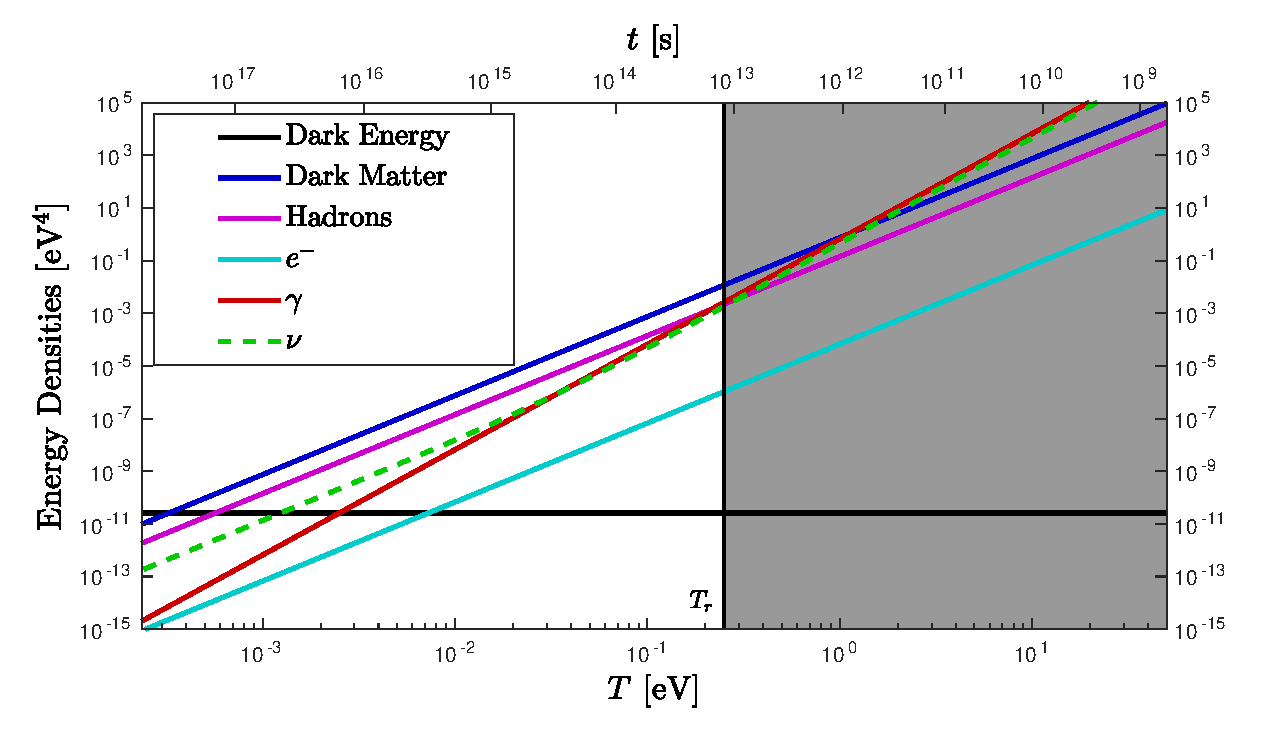
\includegraphics[width=\textwidth]{./plots/energy_densities_new.eps}}
  \caption{Contemporary era: $69\%$ dark energy, $26\%$ dark matter, $5\%$ baryons, $<1\%$ photons and neutrinos.  The dashed line shows $1$ massless and $2\times 0.1\eV$ neutrinos (Neutrino mass choice is just for illustration.  Other values are possible). The recombination temperature $T_{r}\approx0.25\eV$ is shown denoting when the universe was opaque seen here as the shaded region. \label{CosmicDensity}}
\end{figure}
%%%%%%%%%%%%%%%%%%%%%%%%%%%%%%%%%%%%%%%
%%%%%%%%%%%%%%%%%%%%%%%%%%%%%%%%%%%%%%%
\subsection{The Five Plasma Epochs}\label{sec:Timeline}
\noindent At an early time in the standard cosmological model, the Universe began as a fireball, filling all space, with extremely high temperature and energy density \cite{Rafelski:2015cxa}. The ultra-relativistic plasma produced in the early Universe contained almost a perfect symmetry between matter and antimatter except for a small discrepancy of one part in $10^{9}$ which remains a mystery today. We repeat the standard wisdom that the known CP-violation in the Standard Model's weak sector is insufficient to explain the baryon asymmetry we see today. Additionally, three conditions are required in cosmology to explain the asymmetry outlined by Sakharov \cite{Sakharov:1967dj,Sakharov:1988vdp}:
\begin{itemize}
    \item Absence of baryonic charge conservation 
    \item Violation of CP-invariance
    \item Non-stationary conditions in absence of local thermodynamic equilibrium
\end{itemize}
In this work we take the baryon asymmetry as given parameter (though an additional comment on the situation in the context of non-equilibria processes is made in \rsec{Summary}). This fireball then underwent several phases changes which dramatically evolved the gross properties of the Universe as it expanded and cooled. Evolutionary processes in the primordial Universe are taken to be adiabatic. We present an overview \rf{CosmicFraction} of particle families across all epochs in the Universe, as a function of temperature and thus time. The comic plasma, after the electroweak symmetry breaking epoch and presumably inflation, occurred in the early Universe in the following sequence:
%%%%%%%%%%%%%%%%%%%%%%%%%%%%%%%%%%%%%%%
\begin{figure}
  \centerline{\hspace*{0.4cm}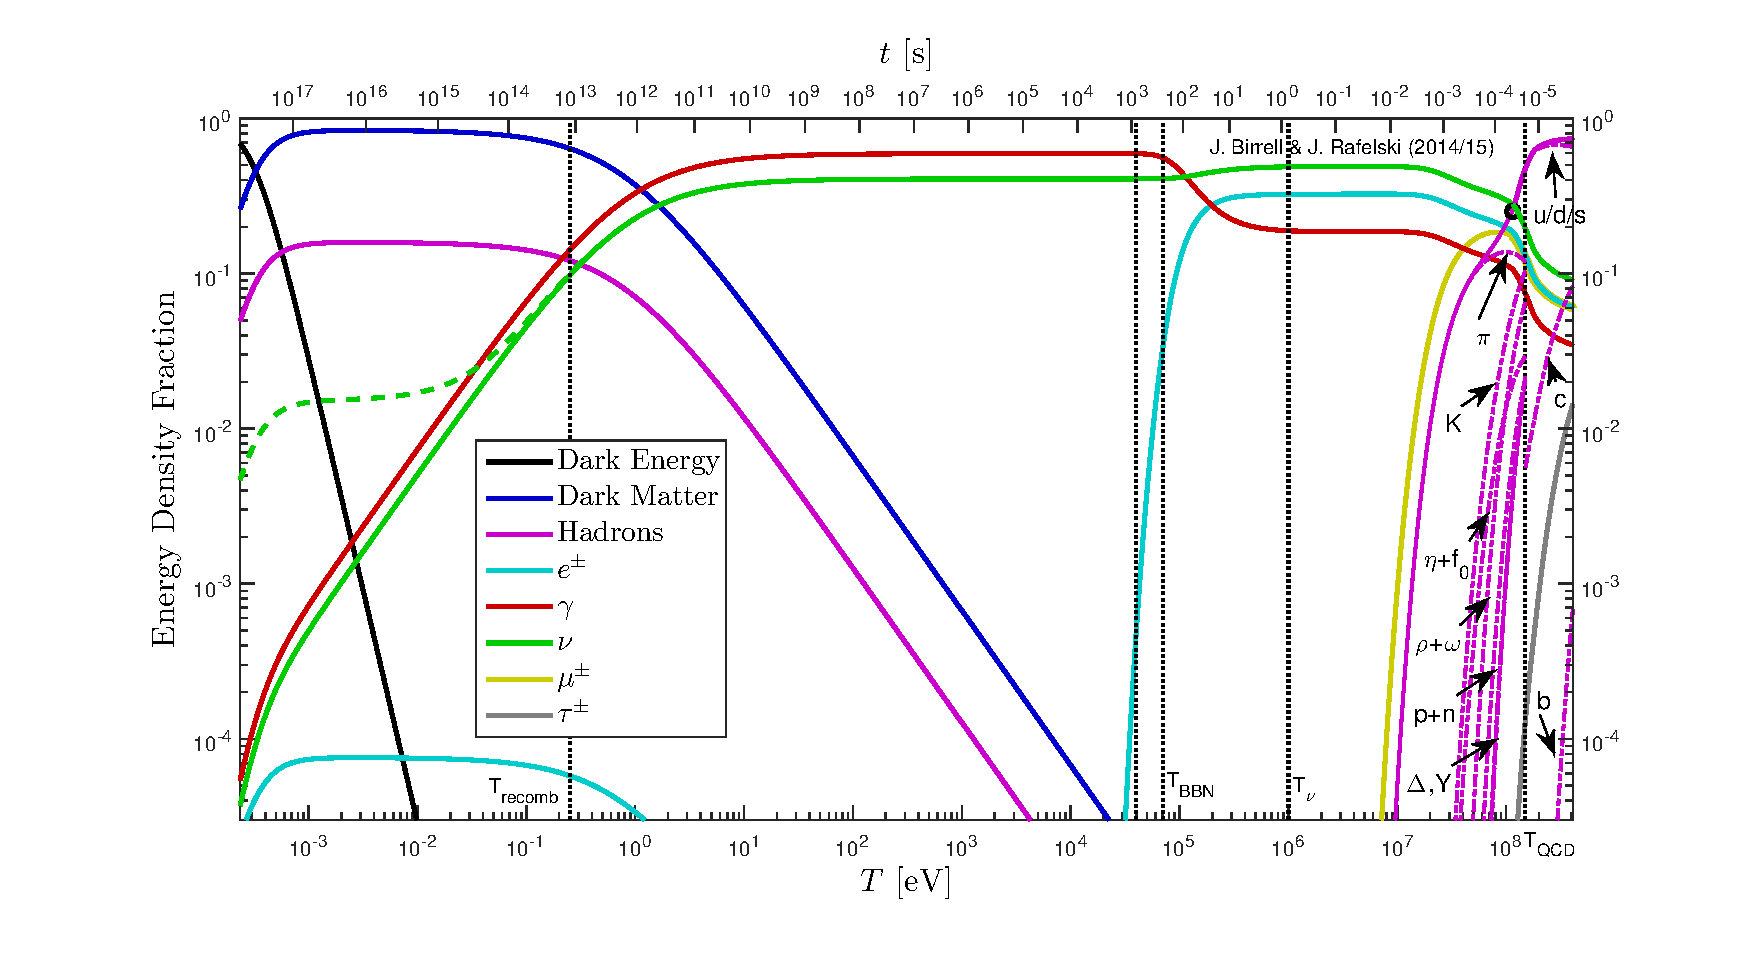
\includegraphics[height=11cm]{./plots/energy_fractions.eps}}
  \caption{Evolution of the differing matter and radiation components of the Universe over cosmological timescales from contemporary observational cosmology to the QGP epoch of the Universe. Key temperatures are listed for specific transitions between epochs. Solid neutrino line shows massless neutrinos while the dashed line shows $1$ massless and $2\times 0.1$ eV neutrinos (Neutrino mass choice is just for illustration.  Other values are possible). \label{CosmicFraction}}
\end{figure}
%%%%%%%%%%%%%%%%%%%%%%%%%%%%%%%%%%%%%%%
\begin{enumerate}
  \item \textbf{Primordial quark-gluon plasma}: At early times when the temperature was between $130\ \mathrm{GeV}>T>150\ \mathrm{MeV}$, we have the building blocks of the Universe as we know them today including the leptons, vector bosons, and all three families of deconfined quarks and gluons which propagated freely. As all hadrons are dissolved into their constituents during this time, strongly interacting particles $u,d,s,t,b,c,g$ controlled the fate of the Universe. Here we will only look at the late-stage evolution at around $150\MeV$.
  \item \textbf{Hadronic epoch}: Around the hadronization temperature $T_h\approx150\ \mathrm{MeV}$, a phase transformation occurred forcing the strongly interacting particles such as quarks and gluons to condense into confined states \cite{Letessier:2005qe,Bazavov:2011nk}. It is here where matter as we know it today forms and the Universe becomes hadronic-matter dominated. In the temperature range $ 150\ \mathrm{MeV}>T>20\ \mathrm{MeV}$ the Universe is rich in physics phenomena involving strange mesons and (anti)baryons including (anti)hyperon abundances \cite{Fromerth:2012fe,Yang:2021bko}.
  \item  \textbf{Lepton-photon epoch}: For temperature $10\ \mathrm{MeV}>T>2\ \mathrm{MeV}$, the Universe contained relativistic electrons, positrons, photons, and three species of (anti)neutrinos. Muons vanish partway through this temperature scale. In this range, neutrinos were still coupled to the charged leptons via the weak interaction. \cite{Birrell:2012gg,Birrell:2014ona}. During this time the expansion of the Universe is controlled by leptons and photons almost on equal footing.
  \item  \textbf{Final antimatter epoch}: After neutrinos decoupled and become free-streaming, referred to as neutrino freezeout, from the cosmic plasma at $T=2\ \mathrm{MeV}$, the cosmic plasma was dominated by electrons, positrons, and photons. We have shown in \cite{Chris:2023abc} that this plasma existed until $T\approx0.02\ \mathrm{MeV}$ such that BBN occurred within a rich electron-positron plasma. This is the last time the Universe will contain a significant fraction of its content in antimatter.
  \item \textbf{Moving towards a matter dominated Universe}: The final major plasma stage in the Universe began after the annihilation of the majority of $e^{\pm}$ pairs leaving behind a residual amount of electrons determined by the baryon asymmetry in the Universe and charge conservation. The Universe was still opaque to photons at this point and remained so until the recombination period at $T\approx0.25\ \mathrm{eV}$ starting the era of observational cosmology with the CMB. This final epoch of the primordial Universe will not be described in detail here, but is well covered in \cite{Planck:2018vyg}.
\end{enumerate}
%%%%%%%%%%%%%%%%%%%%%%%%%%%%%%%%%%%%%%%
\begin{figure}[ht]
  %\begin{center}
  \centering
  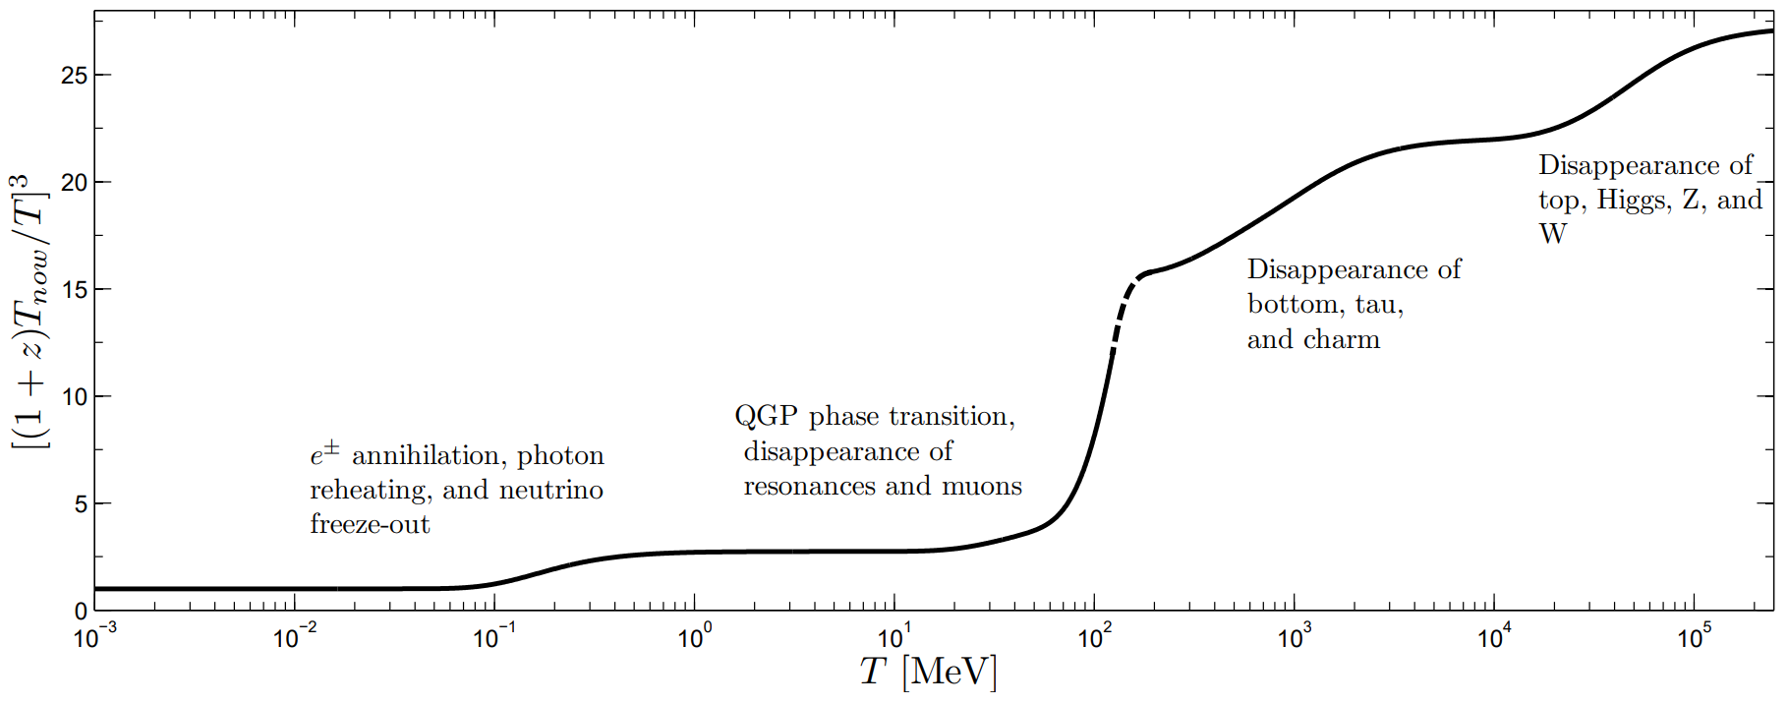
\includegraphics[width=\textwidth]{./plots/degrees_of_freedom}
  \caption{The evolution of the photon reheating (black line) process in terms of fractional temperature change in the Universe. Figure adapted from \cite{Rafelski:2013yka}. The dashed portion is a qualitative description subject to the exact model of QGP hadronization.}
  \label{degrees_of_freedom} 
\end{figure}
%%%%%%%%%%%%%%%%%%%%%%%%%%%%%%%%%%%%%%%

Each plasma outlined above contributes to the thermal behavior of the Universe over time. This is illustrated in \rf{degrees_of_freedom} where the fractional drop in temperature during each plasma transformation is plotted. Each subsequent plasma lowers the available degrees of freedom (as the particle inventory is whittled away) as the Universe cools \cite{Wantz:2009it,Rafelski:2013yka}. Each drop in degrees of freedom represents entropy being pumped into the photons as entropy is conserved (up until gravitational processes become relevant) in an expanding Universe. As there are no longer degrees of freedom to consume reheating the photon field further, the fractional temperature remains constant today.

In Figure \ref{CosmicFraction} we begin on the right at the end  of the QGP era.  The first dotted vertical line shows the QGP phase transition and hadronization, near $T=150\MeV$. The hadron era proceeds with the disappearance of muons, pions, and heavier hadrons. This constitutes a reheating period, with energy and entropy from these particles being transferred to the remaining $e^\pm$, photon, neutrino plasma. The black circle near $T=115\MeV$ denotes our change from $2+1$-flavor lattice QCD \cite{Kronfeld:2012ym, DElia:2012ifm, Bonati:2013hsa} data for the hadron energy density, taken from Borsanyi et al.~\cite{Borsanyi:2012rr,Borsanyi:2013bia}, to an ideal gas model \cite{Bernstein:1988bw} at lower temperature.  We note that the hadron ideal gas energy density matches the lattice results to less than a percent at $T=115\MeV$ \cite{Philipsen:2012nu}. 

To the right of the QGP transition region, the solid hadron line shows the total energy density of quarks and gluons. From top to bottom, the dot-dashed hadron lines to the right of the transition show the energy density fractions of $2+1$-flavor (u,d,s) lattice QCD matter (almost indistinguishable from the total energy density), charm, and bottom (both in the ideal gas approximation).  To the left of the transition the dot-dashed lines show the  pion, kaon, $\eta+f_0$, $\rho+\omega$, nucleon,  $\Delta$, and Y contributions to the energy fraction.

Continuing to the second vertical line at $T=\mathcal{O}(1\, \MeV)$, we come to the annihilation  of $e^\pm$ and the photon reheating period.  Notice that only the photon energy density fraction increases here, as we assume here that neutrinos are already decoupled at this time and hence do not share in the reheating process, leading to a difference in photon and neutrino temperatures. This is not strictly correct but it is a reasonable simplifying assumption for the current purpose; see \cite{Mangano:2005cc,Fornengo:1997wa,Mangano:2001iu,Birrell:2012gg}.  We next pass through a long period, from $T=\mathcal{O}(1\, \MeV)$ until $T=\mathcal{O}(1\, \eV)$, where the energy density is dominated by photons and free-streaming neutrinos.  BBN occurs in the approximate range $T=40-70\keV$ and is indicated by the next two vertical lines.  It is interesting to note that, while the hadron fraction is insignificant at this time, there is still a substantial background of $e^\pm$ pairs during BBN as seen in \rf{Density_fig} and until $T_{\mathrm{split}} = 20.36\ \mathrm{keV}$. For $T<T_{\mathrm{split}}$ the positron density quickly vanishes because of annihilation leaving only a residual electron density as required by charge conservation. 

%%%%%%%%%%%%%%%%%%%%%%%%%%%%%%%%%%%%%%%
\begin{figure}[ht]
  %\begin{center}
  \centering
  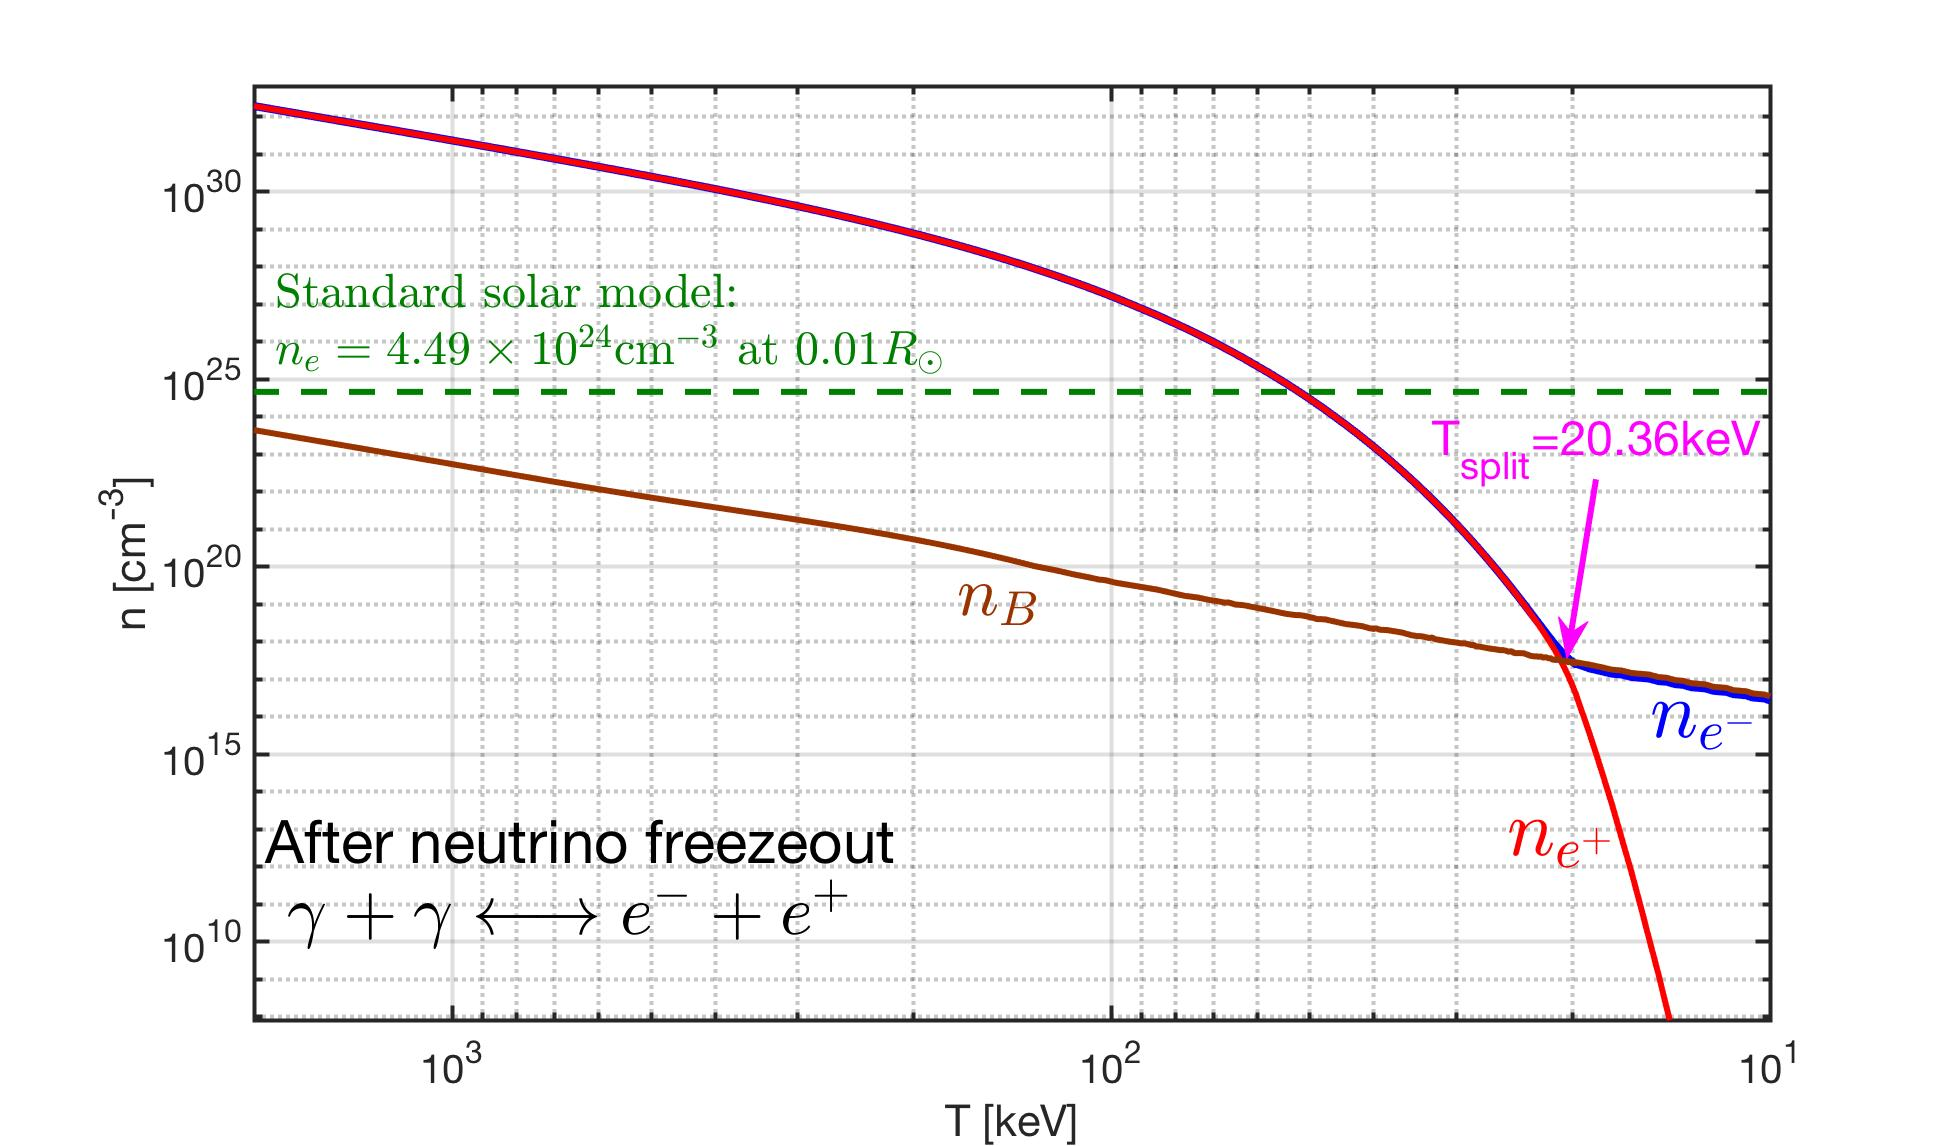
\includegraphics[width=\textwidth]{./plots/NewDensity_cm3.jpg}
  \caption{The $e^{\pm}$ number densities as a function of temperature in the range $2\,\mathrm{MeV}>T>10\,\mathrm{keV}$. The blue solid line is the electron density, the red solid line is the positron density, and the brown solid line is the baryon density. For comparison, we also show the green dotted line as the solar electron density within the solar core \cite{Bahcall:2000nu}.}
  \label{Density_fig} 
\end{figure}
%%%%%%%%%%%%%%%%%%%%%%%%%%%%%%%%%%%%%%%

We then come to the beginning of the matter dominated regime, where the energy density is dominated by the combination of dark matter and baryonic matter.  This transition is the result of the redshifting of the photon and neutrino energy, $\rho\propto a^{-4} \propto T^4$, whereas for non-relativistic matter $\rho\propto a^{-3}\propto T^3$.  Recombination and photon decoupling occurs near the transition to the matter dominated regime, denoted by the vertical line at $T=0.25\eV$.

Finally, as we move towards the present day CMB temperature of $T_{\gamma,0}=0.235$ meV on the left hand side, we have entered the dark energy dominated regime.  For the present day values, we have used the energy densities proscribed by the Planck parameters \cite{Planck:2013pxb} using \req{Planck_params} and zero Universe spatial curvature. The photon energy density is fixed by the CMB temperature $T_{\gamma,0}$ and the neutrino energy density is fixed by $T_{\gamma,0}$ along with the photon to neutrino temperature ratio and neutrino masses.  Both constitute $<1\%$ of the current energy budget.

The Universe evolution and total energy densities were computed using massless neutrinos, but  for comparison we show the energy density of massive neutrinos in the dashed green line. For the dashed line we used two neutrino flavors with masses $m_\nu=0.1\eV$ and one massless flavor.  Note that the inclusion of neutrino mass causes the leveling out of the neutrino energy density fraction during the matter dominated period, as compared to the continued redshifting of the photon energy.

\subsection{The Lambda-CDM Universe}\label{sec:Cosmo}
%%%%%%%%%%%%%%%%%%%%%%%%%%%%%%%
\noindent Here we provide background on the standard $\Lambda$-CDM cosmological (FLRW-Universe) model that is used in the computation of the composition of the Universe over time. We use the spacetime metric with metric signature $(+1,-1,-1,-1)$ in spherical coordinates
\beqn\label{metric}
ds^2=c^2dt^2-a^2(t)\left[ \frac{dr^2}{1-kr^2}+r^2(d\theta^2+\sin^2(\theta)d\phi^2)\right]
%g_{00}=1, \quad g_{rr}=-\frac{a^2}{1-kr^2}, \quad g_{\theta\theta}=-a^2r^2, \quad g_{\phi\phi}=-a^2 r^2\sin^2\theta
\eeqn
characterized  by the scale parameter $a(t)$  of a spatially homogeneous  Universe. The geometric parameter $k$ identifies the Gaussian geometry of the spacial hyper-surfaces defined by co-moving observers. Space is a Euclidean flat-sheet for the observationally preferred value $k=0$ \cite{Planck:2013pxb,Planck:2015fie,Planck:2018vyg}. In this case it can be more convenient to write the metric in rectangular coordinates
\beqn\label{metric2}
ds^2=c^2dt^2-a^2(t)\left[ dx^2+dy^2+dz^2\right].
\eeqn
We will work in units where $\hbar=1,\ c=1$.

The global Universe dynamics can be characterized by two  quantities: the Hubble parameter  $H$, a strongly time dependent quantity on cosmological time scales,  and the deceleration parameter $q$:
\begin{align}
  \label{Hubble} H(t)^{2}&\equiv\left(\frac{\dot a}{a}\right)^2=\frac{8\pi G_{N}}{3}\rho_{tot}\,,\\
  \label{Deceleration} \frac{\ddot a}{a}=-qH^2,\qquad\qquad q&\equiv -\frac{a\ddot a}{\dot a^2},\qquad\qquad \dot H=-H^2(1+q)\,,    
\end{align}
where $G_{N}$ is the Newtonian gravitational constant and $\rho_{tot}$ is the energy density of the Universe and composed of the various energy densities in the Universe. The deceleration parameter $q$ is defined in terms of the second derivative of the scale parameter. In \rf{deceleration_evolution} (left) we illustrate the late stage evolution of the parameters $H$ and $q$ given in \req{Hubble} and \req{Deceleration} compared to temperature. This illustrates how the Universe evolves according to the Friedmann equations \req{Hubble} and \req{Deceleration} above. The deceleration begins radiation dominated with $q=1$ and then transitions to matter dominated $q=1/2$. The contemporary Universe is undergoing the transition from matter dominated to dark energy dominated where, barring the possibility of phantom energy, the deceleration will settle on the asymptotic value of $q=-1$ \cite{Rafelski:2013yka}. Part of the program of this survey is to connect this picture of late stage evolution to the very early universe during and prior to BBN. The current tension in Hubble parameter measurements \cite{Perivolaropoulos:2021jda,DiValentino:2021izs,Aluri:2022hzs}
might benefit from closer inspection of the earlier denser periods. Additionally, the JWST has recently discovered that galaxy formation began earlier than predicted which requires reevaluation of early Universe matter inhomogeneities \cite{Yan:2022sxd}. \rf{deceleration_evolution} (right) shows the close relationship between the redshift $z$ and the Hubble parameter. Deviations separating the two occur from the transitions which changed the deceleration value.

%%%%%%%%%%%%%%%%%%%%%%%%%%%%%%%%%%%%%%%
\begin{figure}[ht]
  %\begin{center}
  \centering
  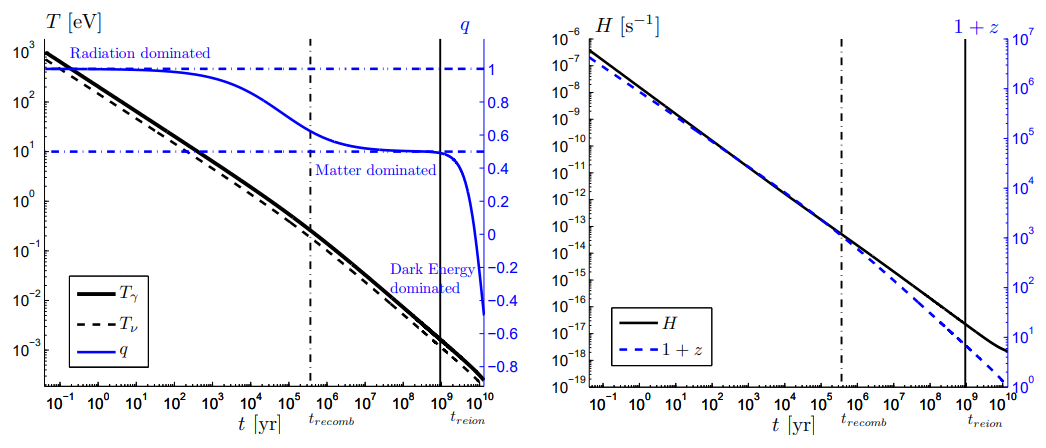
\includegraphics[width=\textwidth]{./plots/deceleration_evolution}
  \caption{ (left) The numerically solved later $t>10^{-1}\ \mathrm{yr}$ evolution of photon and neutrino background temperatures $T_{\gamma},\ T_{\nu}$ (black and black dashed lines) and the deceleration parameter $q$ (thin blue line) over the lifespan of the Universe. (right) The evolution of the Hubble parameter $1/H$ (black line) and redshift $z$ (blue dashed line) which is related to the scale parameter $a(t)$. Figure reprinted from \cite{Rafelski:2013yka}.}
  \label{deceleration_evolution} 
\end{figure}
%%%%%%%%%%%%%%%%%%%%%%%%%%%%%%%%%%%%%%%

The Einstein equations with a cosmological constant $\Lambda$ corresponding to dark energy are:
\beqn\label{Einstein}
G^{\mu\nu}=R^{\mu\nu}-\left(\frac R 2 +\Lambda\right) g^{\mu\nu}=8\pi G_N T^{\mu\nu},  
\quad R= g_{\mu\nu}R^{\mu\nu}.
\eeqn
The homogeneous and isotropic symmetry considerations imply that the stress energy tensor is determined by an energy density and an isotropic pressure
\begin{align}
 T^\mu_\nu =\mathrm{diag}(\rho, -P, -P, -P).
\end{align}
It is common to absorb the Einstein cosmological constant $\Lambda$ into the energy and pressure
\beqn\label{EpsLam}
\rho_\Lambda=\frac{\Lambda}{8\pi G_N}, \qquad P_\Lambda=-\frac{\Lambda}{8\pi G_N}
\eeqn
and we implicitly consider this done from now on.

Two dynamically independent Friedmann equations \cite{weinberg1972gravitation} arise using the metric \req{metric} in \req{Einstein}:
\beqn\label{hubble}
\frac{8\pi G_N}{3} \rho =  \frac{\dot a^2+k}{a^2}
=H^2\left( 1+\frac { k }{\dot a^2}\right),
\qquad
\frac{4\pi G_N}{3} (\rho+3P)  =-\frac{\ddot a}{a}=qH^2.
\eeqn
We can eliminate the strength of the interaction, $G_N$,  solving both these equations for ${8\pi G_N}/{3}$, and equating the result to find a relatively simple constraint for the deceleration parameter:
\beqn\label{qparam}
q=\frac 1 2 \left(1+3\frac{P}{\rho}\right)\left(1+\frac{k}{\dot a^2}\right).
\eeqn
For a spatially flat Universe, $k=0$, note that in a  matter-dominated era where $P/\rho<<1$ we have $q\simeq 1/2$; for a radiative Universe where $3P=\rho$ we find $q= 1 $; and  in a dark energy Universe in which $P=-\rho$  we find $q=-1$.  Spatial flatness is equivalent to the assertion that the energy density of the Universe equals the critical density
\begin{equation}\label{crit_density}
\rho=\rho_{\text{crit}}\equiv \frac{3H^2}{8\pi G_N}.
\end{equation}

 The CMB power spectrum is sensitive to the  deceleration parameter  and the presence of spatial curvature modifies $q$. The Planck results~\cite{Planck:2013pxb,Planck:2015fie,Planck:2018vyg} constrain  the effective curvature energy density fraction,
\begin{equation}
\Omega_K\equiv1-\rho/\rho_{\text{crit}},
\end{equation}
to
\begin{equation}
|\Omega_K|<0.005.
\end{equation}
This indicates a nearly flat Universe which is spatially Euclidean. We will work here within an exactly spatially flat cosmological model, $k=0$.  


As must be the case for any solution of Einstein's equations,   \req{hubble} implies that the energy momentum tensor of matter is divergence free:
\beqn\label{divTmn}
T^{\mu\nu};_\nu =0 \Rightarrow -\frac{\dot\rho}{\rho+P}=3\frac{\dot a}{a}=3H.
\eeqn
A dynamical evolution equation for $\rho(t)$ arises once we combine \req{divTmn} with \req{hubble},  eliminating $H$.   Given an equation of state $P(\rho)$, solutions of this equation describes the dynamical evolution of matter in the Universe. In practice, we evolve the system in both directions in time.  On one side, we start in the present era with the energy density fractions fit by Planck data \cite{Planck:2013pxb},
\begin{equation}\label{Planck_params}
H_0=67.74\text{km/s/Mpc},\hspace{2mm} \Omega_b=0.05,\hspace{2mm} \Omega_c=0.26, \hspace{2mm}\Omega_\Lambda=0.69,
\end{equation}
 and integrate backward in time. On the other hand, we start in the QGP era with an equation of state determined by an ideal gas of SM particles, combined with a perturbative QCD equation of state for quarks and gluons \cite{Borsanyi:2013bia}, and integrate forward in time. As the Universe continues to dilute from dark energy in the future, the cosmic equation of state is becoming well approximated by the de Sitter inflationary metric which is a special case of FLRW.



%%%%%%%%%%%%%%%%%%%%%%%%%%%%%%%%%%%%%%%
\section{QGP Epoch}\label{sec:QGP}
\subsection{Conservation Laws in QGP}\label{sec:Conservation}
\noindent During the first $\approx30\ \mu$sec after the Big Bang, the early Universe is a hot soup that containing the elementary primordial building blocks of matter \cite{Rafelski:2015cxa}. In particular it contained the light quarks which are now hidden in protons and neutrons. Beyond this there were also electrons, photons, neutrinos, and massive strange and charm quarks. These interacting particle species were kept in chemical and thermal equilibrium with one another. Gluons which mediated the color interaction are very abundant as well. This primordial phase lasted as long as the temperature of the Universe was more than 110,000 times than the expected temperature $T_{\odot}=1.36\keV\ (1.58\times10^{7}\ \mathrm{K})$ at the center of the Sun \cite{Castellani:1996cm}.

%%%%%%%%%%%%%%%%%%%%%%%%%%%%%%%%%%%%%%%
\begin{figure}[ht]
  %\begin{center}
  \centering
  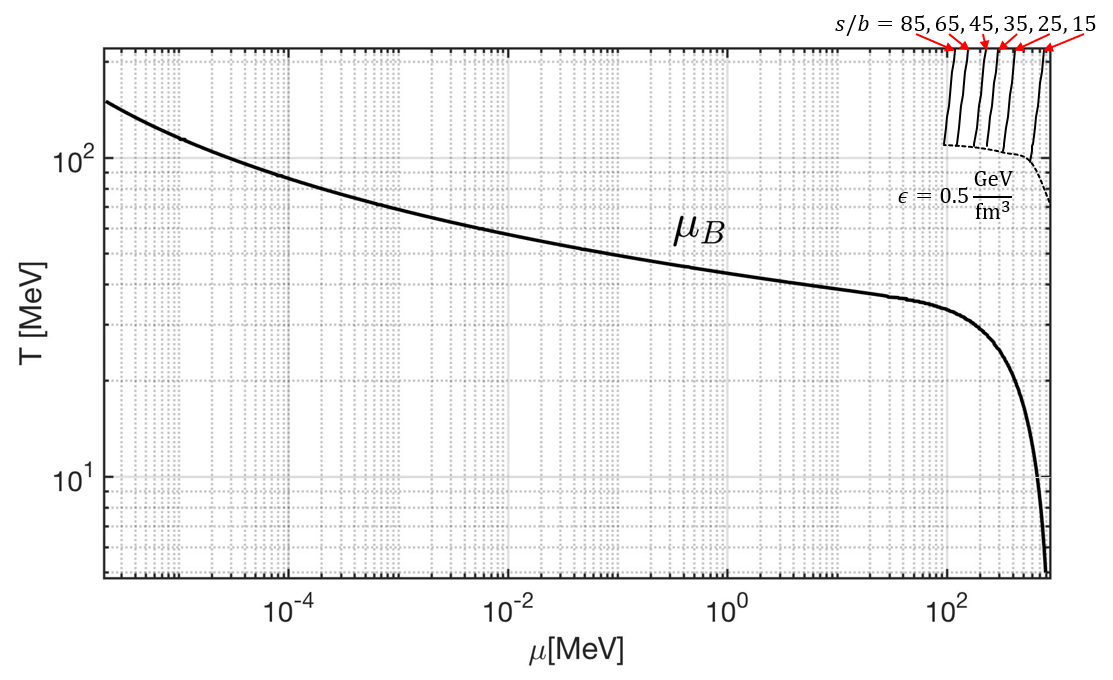
\includegraphics[width=\textwidth]{./plots/phaseQGP}
  \caption{The evolution of the cosmic baryon chemical potential $\mu_{B}$ after hadronization (black line). Curves for QGP (thin black line) created in terrestrial accelerators for differing entropy-per-baryon $s/B$ values are included \cite{Rafelski:1987nv}. The boundary (dashed line) where QGP condenses into hadrons is illustrated at an energy density of $0.5\GeV/\mathrm{fm}^{3}$ as determined through lattice computation \cite{HotQCD:2014kol}.}
  \label{phaseQGP} 
\end{figure}
%%%%%%%%%%%%%%%%%%%%%%%%%%%%%%%%%%%%%%%


The conditions in the early universe and those created in relativistic collisions of heavy atomic nuclei differ somewhat: whereas the primordial quark-gluon plasma survives for about 30 $\mu$sec in the Big Bang, the comparable extreme conditions created in ultra-relativistic nuclear collisions are extremely short-lived \cite{Rafelski:2001hp} on order of $10^{-23}$ seconds. As a consequence of the short lifespan of laboratory QGP in heavy-ion collisions \cite{Ollitrault:1992bk,Petran:2013lja}, they are not subject to the same weak interaction dynamics \cite{Ryu:2015vwa} as the characteristic times for weak processes are too lengthy \cite{Rafelski:1982ii}. Therefore our ability to recreate the conditions of the primordial QGP are limited due to the relativistic explosive disintegration of the extremely hot dense relativistic `fireballs' created in modern accelerators. This disparity is seen in \rf{phaseQGP} where the chemical potential of QGP $\mu_{q}=\mu_{B}/3$ \cite{Rafelski:1987nv} for various values of entropy-per-baryon $s/B$ relevant to relativistic particle accelerators are plotted alongside the evolution of the cosmic hadronic plasma chemical potential. The confinement transition boundary (dashed line in \rf{phaseQGP}) was calculated using a $(u,d,s)$ bag model \cite{Letessier:2002ony} which has good agreement with lattice results \cite{HotQCD:2014kol}. The QGP precipitates hadrons in cosmic fluid at a far higher entropy ratio than those accessible by terrestrial means and the two manifestations of QGP live far away from each other on the QCD phase diagram \cite{Braun-Munzinger:2008szb,Bazavov:2009zn,Jacak:2012dx}.

The work of Fromerth et. al. \cite{Fromerth:2012fe} allows us to parameterize the chemical potentials $\mu_d$, $\mu_e$, and $\mu_\nu$ during this epoch as they are the lightest particles in each main thermal category: quarks, charged leptons, and neutral leptons. The quark chemical potential is determined by the following three constraints \cite{Fromerth:2012fe}:
%%%%%%%%%%%%%%%%%%%%%%%%%%%%%%%%%%%%%%%
\begin{figure}[ht]
  %\begin{center}
  \centering
  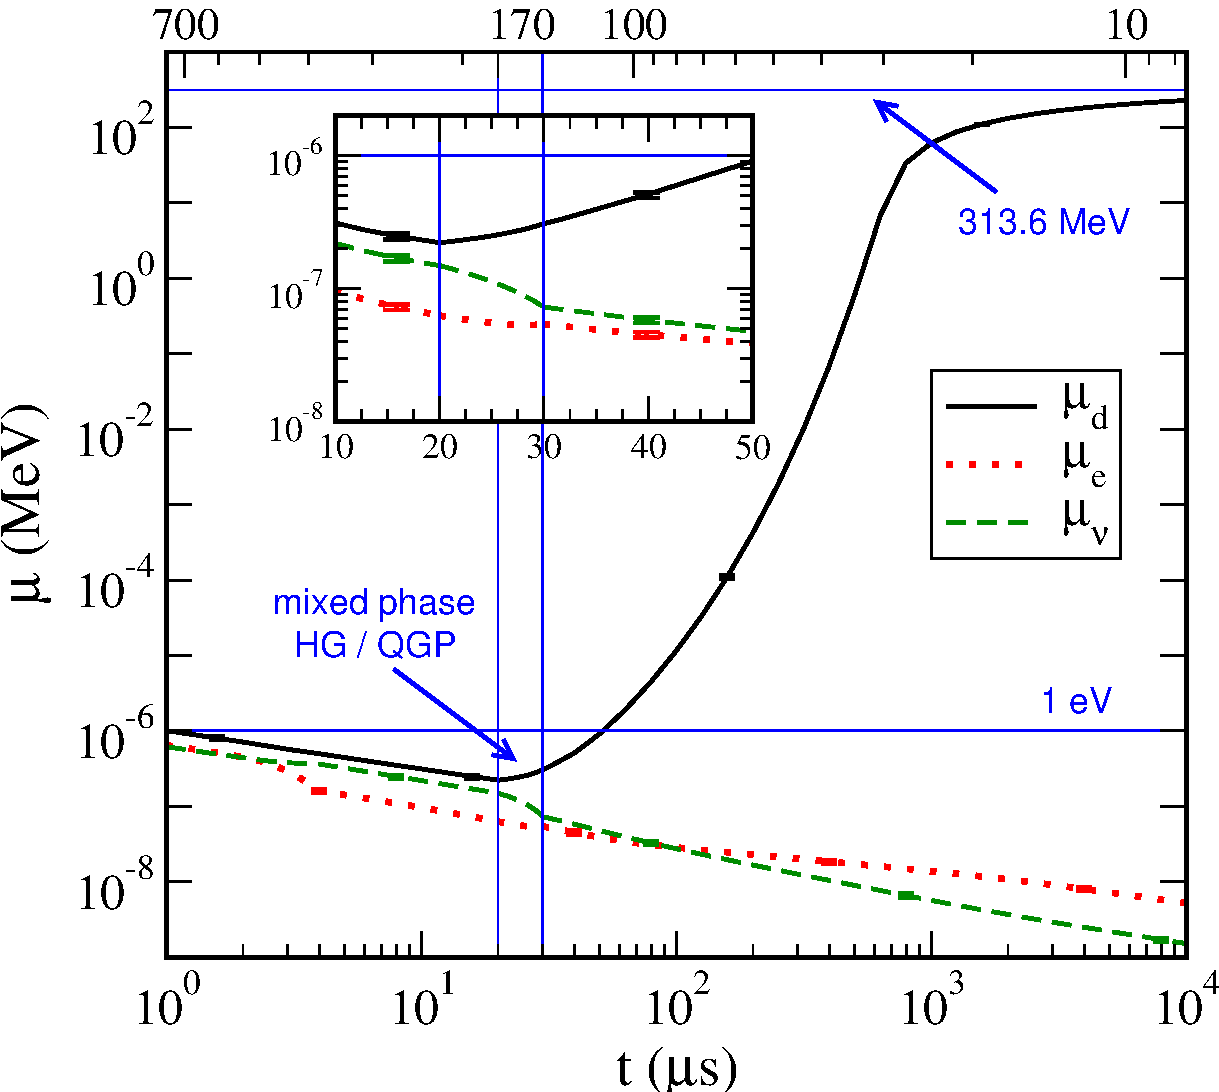
\includegraphics[width=\textwidth]{./plots/muCombo.pdf}
  \caption{Plot of the down quark chemical potential (black), electron chemical potential (dotted red) and neutrino chemical potential (dashed green) as a function of time. (2003 unpublished, Fromerth \& Rafelski) \cite{Rafelski:2019twp}}
  \label{QGPchem1} 
\end{figure}
%%%%%%%%%%%%%%%%%%%%%%%%%%%%%%%%%%%%%%%
\begin{enumerate}
\item Electric charge neutrality $Q=0$, given by
\begin{align}\label{QGP_Q}
    Q\equiv\sum_f\,Q_f\,n_f(\mu_f,T)=0
\end{align}
where $Q_f$ is the charge and $n_{f}$ is the numerical density of each species $f$. $Q$ is a conserved quantity in the Standard Model under global $U(1)_{EM}$ symmetry. This is summed is over all particles present in the QGP epoch.
\item Baryon number and lepton number neutrality $B-L=0$, given by
\begin{align}\label{QGP_LB}
B-L\equiv\sum_f(B_f-L_f)n_f(\mu_f,T)=0
\end{align}
where $L_f$ and $B_f$ are the lepton and baryon number for the given species $f$. This condition is phenomenologically motivated by baryogenesis and is exactly conserved in the Standard Model under global $U(1)_{B-L}$ symmetry. We note many Beyond-Standard-Model (BSM) models also retain this as an exact symmetry though Majorana neutrinos do not.
\item The entropy-per-baryon ratio $s/n_B$ is a constant and can be written as
\begin{align}\label{QGP_sB}
\frac{s}{n_B}=\frac{\sum_fs_f(\mu_f,T)}{\sum_fB_fn_f(\mu_f,T)}=\mathrm{const}
\end{align}
where $s_f$ is the entropy density of given species $f$. As the expanding Universe remains in thermal equilibrium, the entropy is conserved within a co-moving volume. The baryon number within a co-moving volume is also conserved. As both quantities dilute with $1/a(t)^{3}$ within a normal volume, the ratio of the two is constant. This constraint does not become broken until spatial inhomogeneitiess from gravitational attraction becomes significant leading to increases in local entropy.
\end{enumerate}
At each temperature $T$, the above three conditions form a system of three coupled, nonlinear equations of the three chosen unknowns (here we have $\mu_d$, $\mu_e$, and $\mu_\nu$). In \rf{QGPchem1} we present numerical solutions to the conditions \req{QGP_Q}-\req{QGP_sB} and plot the chemical potentials as a function of time. As seen in the figure, the three potentials are in alignment during the QGP phase until the hadronization epoch where the down quark chemical potential diverges from the leptonic chemical potentials before reaching an asymptotic value at late times. This asymptotic value is given as approximately $1/3$ the mass of the nucleons and represents the confinement of the quarks into the protons and neutrons at the end of hadronization. This asymptotic limit is also shown in \rf{QGPchem2} where we present the down quark chemical potential for different values of the entropy-to-baryon ratio. While the $s/n_{B}$ ratio has large consequences for the plasma at high temperatures, the chemical potential is insensitive to this parameter at low temperatures as it converged to an asymptotic value as the Universe cools. Therefore the entropy to baryon value today greatly controls the quark content when the Universe was very hot. We note that the distribution of quarks in the QGP plasma does not remain fixed to the Fermi-Dirac distribution for thermal and entropic equilibrium. The quark partition function is instead
\begin{align} \label{QuarkDistribution}\ln\mathcal{Z}_{\mathrm{quarks}}=\sum_{q}\ln\left(1+\Upsilon_{q}(t)e^{-\beta E_{q}}\right)\,,\qquad\Upsilon_{q}(t)=\gamma_{q}(t)\lambda_{q}\,\qquad q=u,d,c,s,t,b,
\end{align}
which is summed over all quarks and their quantum numbers. In \req{QuarkDistribution}, $\lambda_{q}$ is the quark fugacity while $\gamma_{q}(t)$ is the temporal inhomogeneity of the population distribution \cite{Rafelski:2019twp}. Because of nuclear reactions, these distributions populate and depopulate over time which pulls the gas off entropic equilibrium while retaining temperature $T$ with the rest of the universe \cite{Letessier:2002ony}. When $\gamma\neq1$, the entropy of the quarks is no longer minimized. As entropy in the cosmic expansion is conserved overall, this means the entropy gain or loss is then related to the entropy moving into the quarks or its products.

In practice, the generalized fugacity is always $\gamma=1$ during the QGP epoch as the quarks in early universe remained in both thermal and entropic equilibrium. This is because the Universe's expansion was many orders of magnitude slower than the process reaction and decay timescales \cite{Letessier:2002ony}. However near the hadronization temperature, heavy quarks abundance and deviations from chemical equilibrium have not yet been studied in great detail. We show in \cite{Yang:2020nne,Yang:2023bot} that the bottom quarks can deviate from chemical equilibrium $\gamma\neq1$ by breaking the detailed balance between reactions of the quarks.
%%%%%%%%%%%%%%%%%%%%%%%%%%%%%%%%%%%%%%%
\begin{figure}[ht]
  %\begin{center}
  \centering
  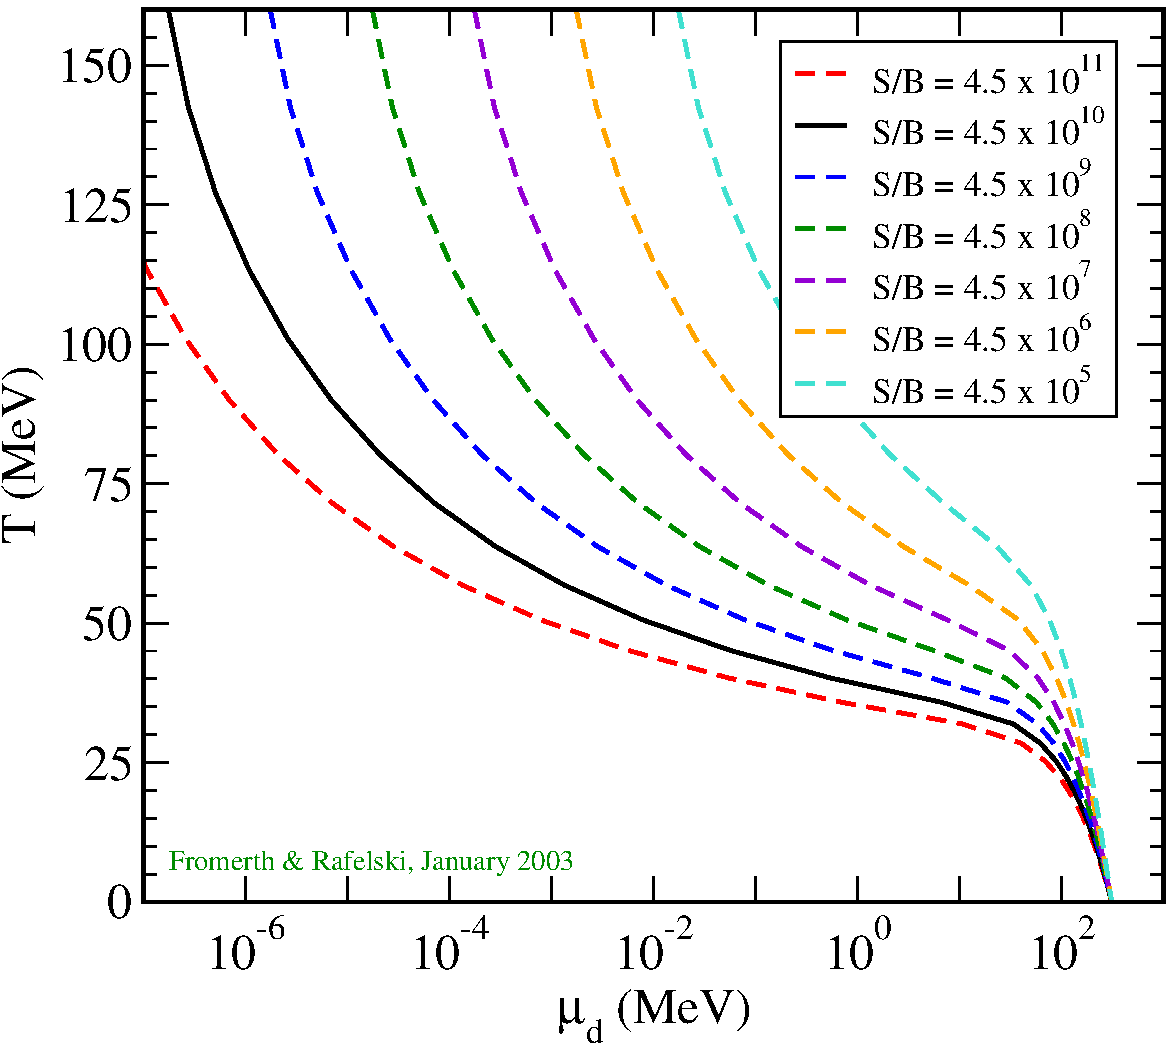
\includegraphics[width=\textwidth]{./plots/Tmud1.pdf}
  \caption{Plot of the down quark chemical potential $\mu_{d}$ as a function of temperature for differing values of entropy-to-baryon $S/B$ ratios. (2003 unpublished, Fromerth \& Rafelski) \cite{Rafelski:2019twp}}
  \label{QGPchem2} 
\end{figure}
%%%%%%%%%%%%%%%%%%%%%%%%%%%%%%%%%%%%%%%

%%%%%%%%%%%%%%%%%%%%%%%%%%%%%%%%%%%%%%%
\subsection{Heavy flavor: bottom and charm in QGP}\label{BottomCharm}
\noindent In the QGP epoch, the up/down are massless quarks and retain the equilibrium via gluon/quark fusion. Strangeness retains the equilibrium via weak, electromagnetic, and strong interaction until $T\sim12$ MeV \cite{Yang:2021bko}. In this section, we focus on the heavy bottom and charm quarks in QGP. In the primordial QGP, the bottom/charm quarks can be produced via the strong interaction gluon/quark pair fusion processes and disappear via the weak interaction decay. We have
\begin{align}
    q+q\longrightarrow b+\bar b, c+\bar c,\qquad g+g\longrightarrow b+\bar b, c+\bar c
\end{align}
for productions and 
\begin{align}
    &b\longrightarrow c+l+\nu_l, \qquad b\longrightarrow c+q+\bar{q}\\
&c\longrightarrow s+l+\nu_l,\qquad c\longrightarrow s+q+\bar{q}
\end{align}
for decay. The detail calculation of production and decay rate can be found in \cite{Yang:2020nne,Yang:2023bot}.
%~~~~~~~Figure~~~~~~~~~~~~~~~~~~~~~~~~~~~~~~~~~~~~~~~~~~~~~~~~~~~
\begin{figure} %[ht]
\begin{center}
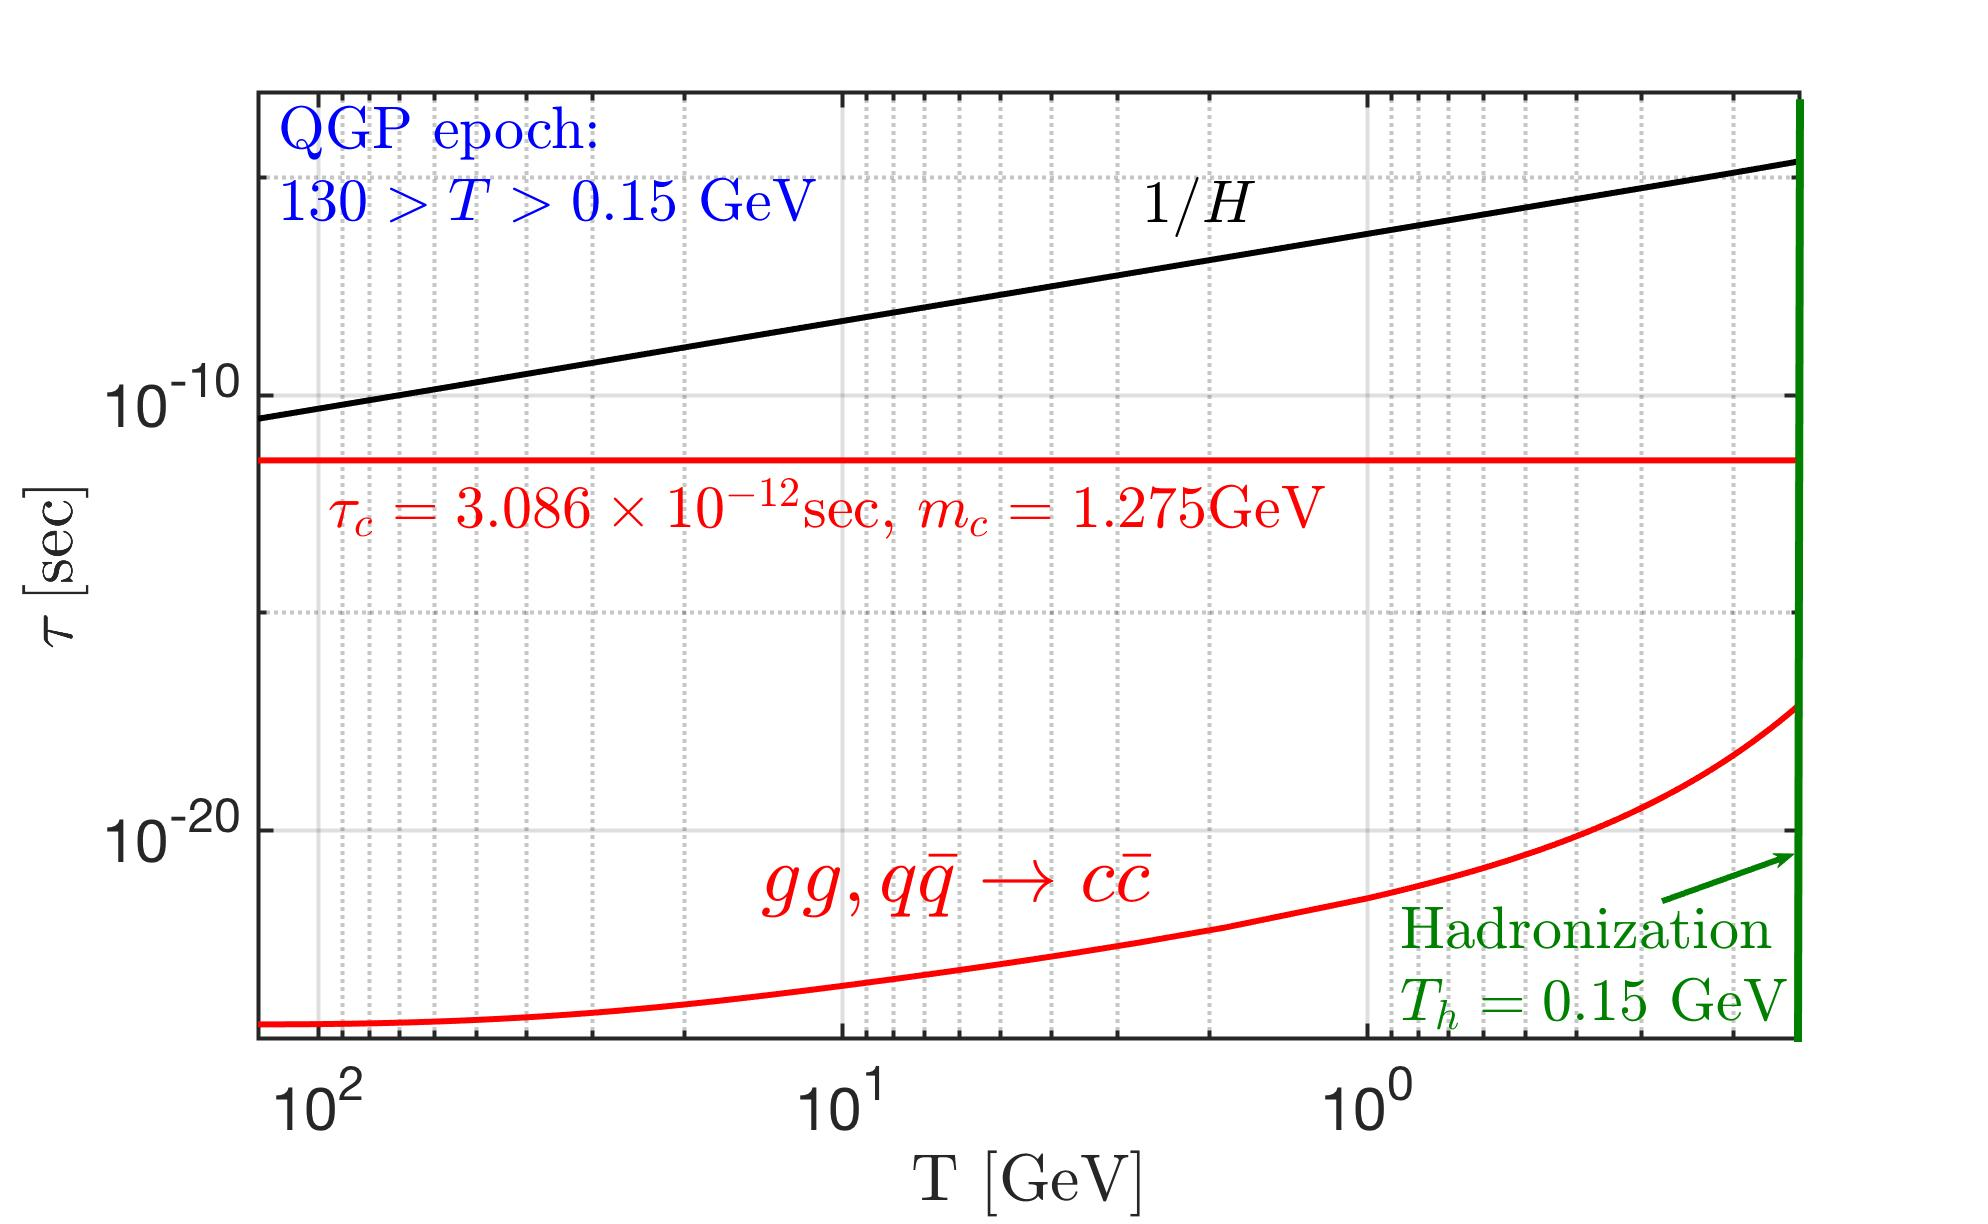
\includegraphics[width=\textwidth]{./plots/CharmQuark_QGP.jpg}\\
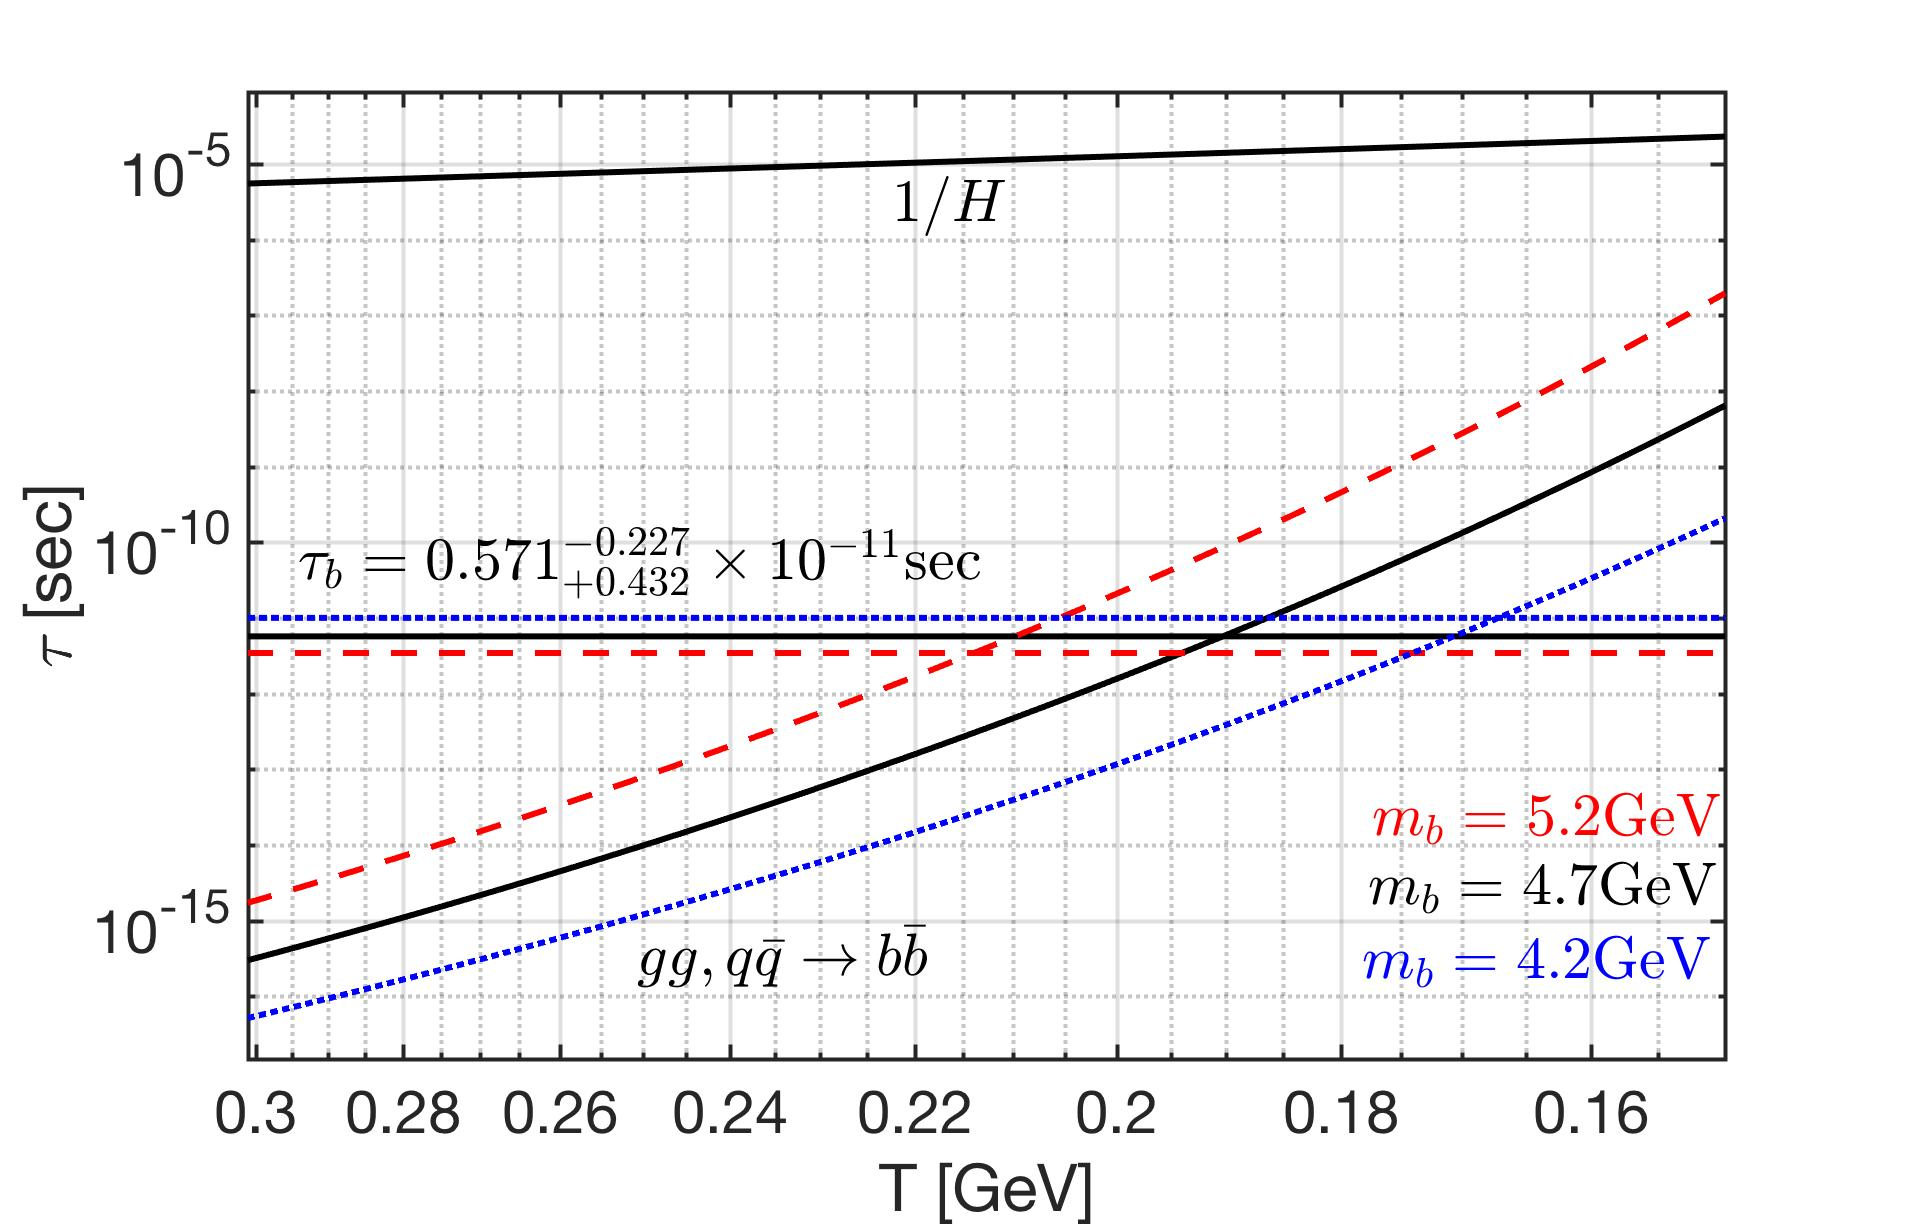
\includegraphics[width=\textwidth]{./plots/BQuarkReactionTime_bottom.jpg}
\caption{ Comparison of Hubble time $1/H$, lifespan, and characteristic time for charm (upper) and bottom (lower) production as a function of temperature. Upper: it shows that the relaxation time for c-quark production is faster than the c-quark decay in QGP. Lower: it shows the competition between production and decay, and  establishes the temperature era for the abundance non-equilibrium of bottom quarks.}
\label{BCreaction_fig}
\end{center}
\end{figure}
%~~~~~~~~~~~~~~~~~~~~~~~~~~~~~~~~~~~~~~~~~~~

In the early Universe within a temperature range $130\, \mathrm{GeV}>T>150\, \mathrm{MeV}$  we have the following particles:  photons, $8_c$-gluons, $W^\pm$, $Z^0$, three generations of $3_c$-quarks and leptons  in the primordial QGP.  The Hubble parameter can be written as the sum of particle energy densities $\rho_i$ for each species
\begin{align}
H^2=\frac{8\pi G_{N}}{3}\left(\rho_\gamma+\rho_{\mathrm{lepton}}+\rho_{\mathrm{quark}}+\rho_{g,{W^\pm},{Z^0}}\right),
\end{align}
where $G_{N}$ is Newton's constant of gravitation. Ultra-relativistic particles (which are effectively massless) and radiation dominate the speed of expansion. The Universe's characteristic expansion time constant $1/H$ is seen in  \rf{BCreaction_fig}. During QGP, the Hubble time is much larger than the lifespan and production times of the bottom and charm quarks. Therefore, these heavier quark species remain in equilibrium as their processes occur much faster than the expansion of the Universe.

In Fig.~\ref{BCreaction_fig} (on top) we plot the relaxation time for production and decay of charm as a function of temperature. It shows the relaxation time for c-quark production is faster than the c-quark decay in QGP epoch, and both production and decay are faster than the Hubble time $1/H$. The faster gluon/quark pair fusion keeps the charm quark in chemical equilibrium until hadronization. After hadronization, charm quarks form heavy mesons that decay into multi-particles very fast. The Charm disappears from particle inventory once the hadronization is formed. %It shows that the massive charm quarks disappear from the universe rapidly after hadronization and can’t contribute to matter genesis.

In Fig.~\ref{BCreaction_fig} (on bottom) we plot the relaxation time for production and decay of the bottom with different masses as a function of temperature. It shows that both production and decay are faster than the Hubble time $1/H$ and the relaxation time for b-quark production intersects with b-quark decay at different temperatures which depend on the mass of the bottom. This means that the bottom quark decoupling from the primordial plasma is driven by the production process slowing down at low temperature and not being able to keep up with the WI-decay rate of bottom quarks, and Hubble expansion rate is not relevance compare to the decay and production rates.
%~~~~~~~Figure~~~~~~~~~~~~~~~~~~~~~~~~~~~~~~~~~~~~~~~~~~~~~~~~~~~
\begin{figure} [t]
%\begin{center}
\centering
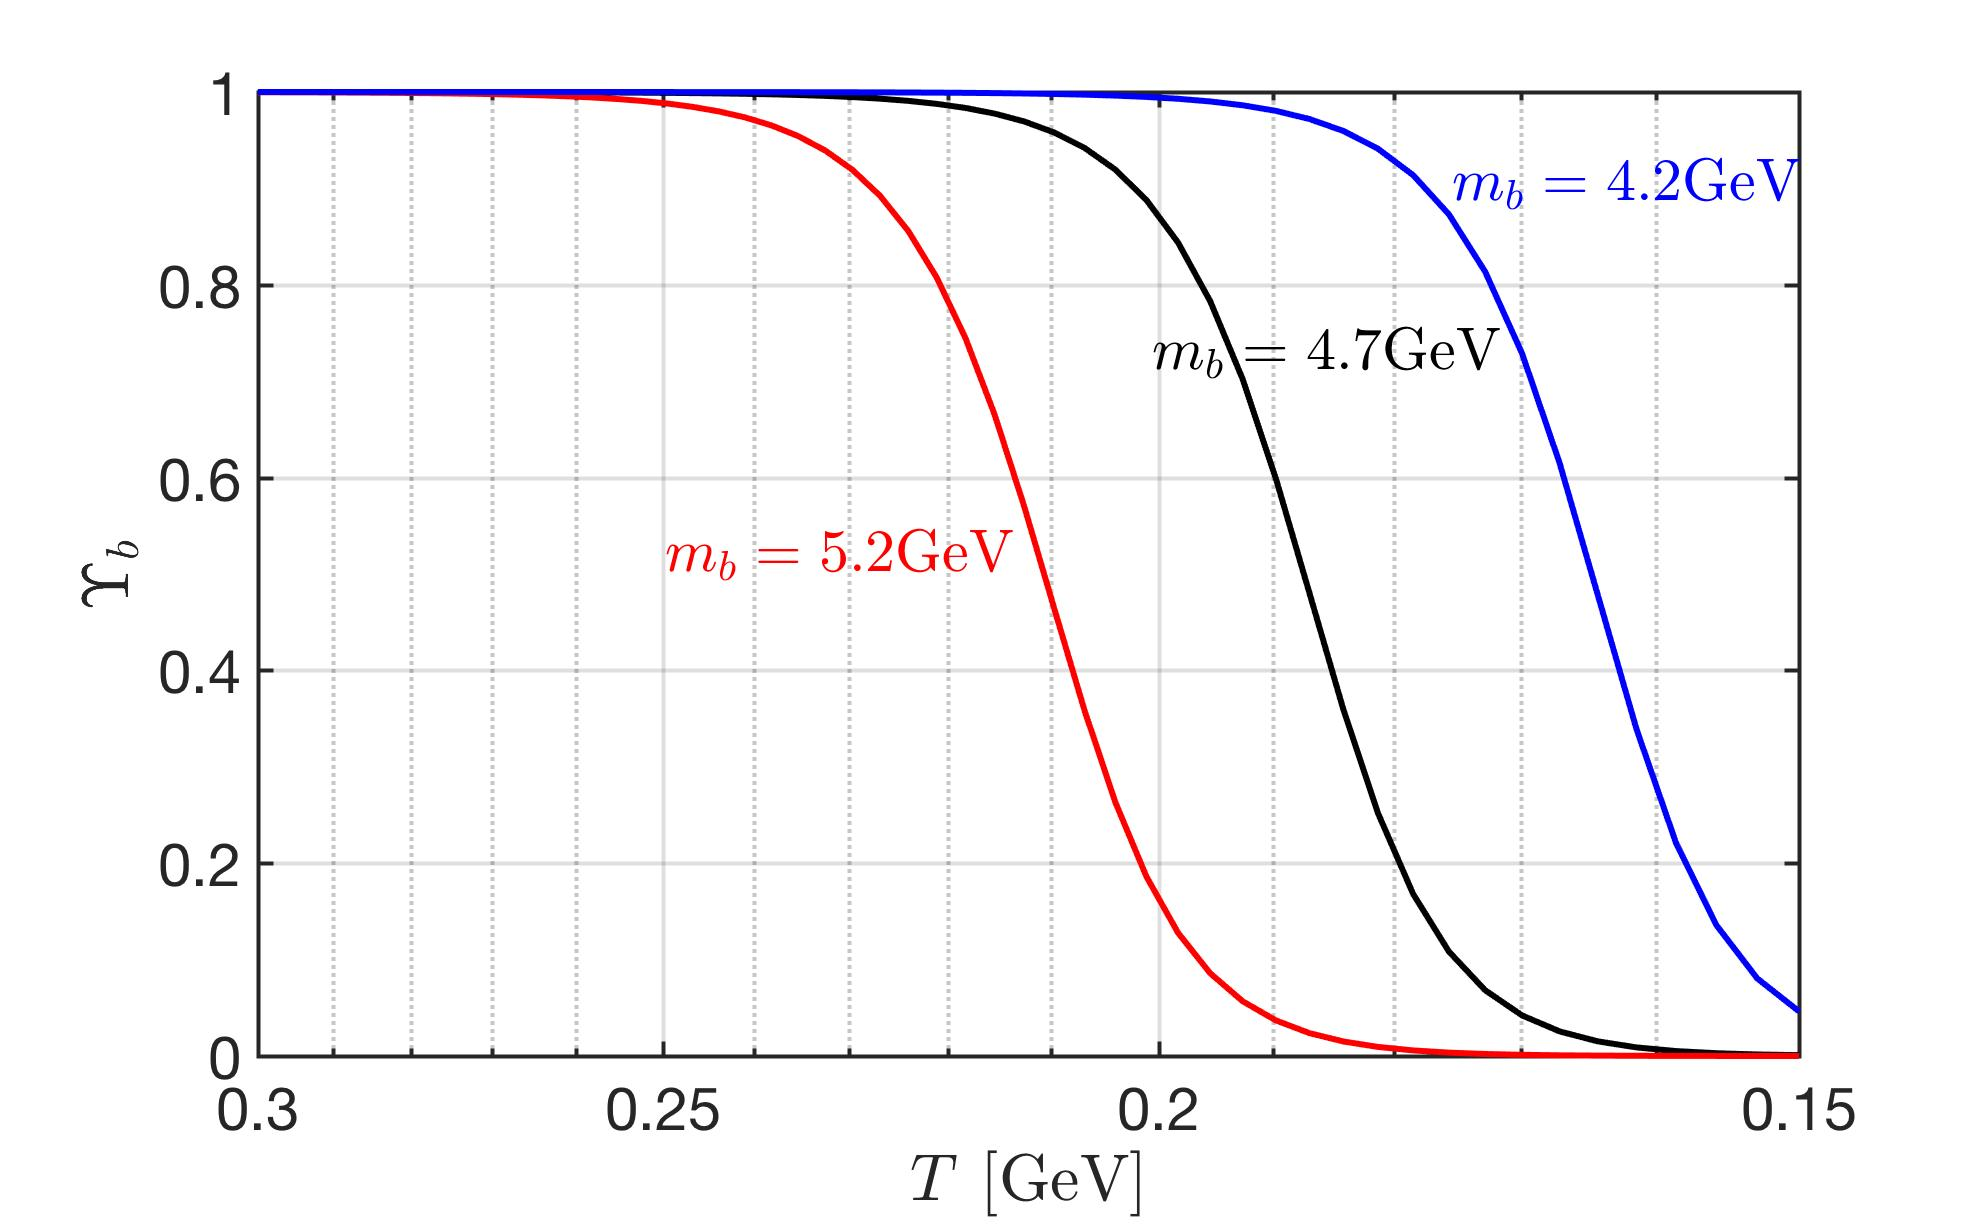
\includegraphics[width=\textwidth]{./plots/BquarkFugacity.jpg}
\caption{The fugacity of free bottom quark as a function of temperature in the early Universe for $m_b = 4.2$GeV (blue), $m_b = 4.7 $GeV (black), and $m_b = 5.2$ GeV (red). The prolonged non-equilibrium happens because the decay and reformation rates of bottom quarks are comparable to each other as the temperature of the universe cools down. }
\label{UpsilonBottom_fig}
%\end{center}
\end{figure}
%~~~~~~~~~~~~~~~~~~~~~~~~~~~~~~~~~~~~~~~~~~~~
The competition between decay and production reactions requires the study of dynamic bottom abundance in QGP. The dynamic equation of bottom abundance in the early universe can be written as
\begin{align}
\label{Bquark_eq}
\frac{1}{V}\frac{dN_b}{dt}=\big(\,1-\Upsilon^2_{b}\,\big)\,R^{\mathrm{Source}}_{b}-\Upsilon_b\,R^{\mathrm{Decay}}_{b}\;,
\end{align}
where $\Upsilon_b$ is the general fugacity of bottom quarks, and $R^{\mathrm{Source}}_{b}$ and $R^{\mathrm{Decay}}_{b}$ are the thermal reaction rates per volume of production and decay of bottom quark, respectively. The bottom source rates are the gluon fusion rate and quark fusion, while the decay rate depends on whether we have free bottom quarks in plasma or they are bounded in the mesons. We study the dynamic equation for bottom abundance and solve the fugacity parameter of the bottom under adiabatic approximation \cite{Yang:2020nne,Yang:2023bot}, we have
\begin{align}
\Upsilon_{b}=\frac{R^{\mathrm{Decay}}_{b}}{2R^{\mathrm{Source}}_{b}}\left[\sqrt{1+\left(2R^{\mathrm{Source}}_{b}/R^{\mathrm{Decay}}_{b}\right)^2}-1\right]
\end{align}

In Fig.(\ref{UpsilonBottom_fig}) we show the fugacity of the bottom quarks as a function of temperature $T=0.3\sim0.15\GeV$ for different masses of bottom quarks. In all cases, we have prolonged non-equilibrium and this happens since the decay and reformation rates of bottom quarks are comparable to each other. It also shows that  the smaller mass of the bottom quark slows the strong interaction formation rate to the value of weak decay near the phase transformation of QGP to HG phase.

In this case, the bottom flavor breaks the detail balance and disappearance from particle inventory during the epoch $T = 0.3 \sim0.15\GeV$ which is the essential condition for departure from the thermal equilibrium. Our results provide a strong motivation to explore the physics of baryon non-conservation involving the bottom quarks or bottonium mesons in a thermal environment. Given that the non-equilibrium of bottom flavor arises at a relatively low QGP temperature allows the possibility for baryogenesis to be occurred in primordial QGP hadronization \cite{Yang:2020nne,Yang:2023bot}. This result is of pivotal importance in the QGP study as it establishes the temperature era for the abundance non-equilibrium of bottom quarks.

%%%%%%%%%%%%%%%%%%%%%%%%%%%%%%%%%%%%%%%
\section{Hadronic Epoch}\label{sec:Hadrons}
\subsection{The Formation of Matter}\label{sec:Creation}
\noindent It is in this epoch that the matter of the universe, including all the baryons which make up visible matter today, was created \cite{Fromerth:2002wb,Rafelski:2019twp}. Unlike the fundamental particles, such as the quarks or W and Z, the mass of these hadrons is not due to the Higgs mechanism, but rather from the condensation of the QCD vacuum \cite{Rafelski:2015cxa,Roberts:2021xnz,Roberts:2022rxm}. The quarks from which protons and neutrons are made have a mass more than 100 times smaller than these nucleons. The dominant matter mass-giving mechanism arises from quark confinement \cite{Hagedorn:1984hz}. Light quarks are compressed by the quantum vacuum structure into a small space domain a hundred times smaller than their natural `size'. That costs a lot of energy which is the nucleon mass. The remaining few percent of mass are than due to the fact that quarks also have inertial mass provided by the Higgs mechanism as well as the electromagnetic mass for particles with charge. At a temperature of $T_{h}\approx150\MeV$ the quarks and gluons became confined condensing into the hadrons (both baryons and mesons). During this period, the number of baryon-antibaryon pairs was sufficiently high that the asymmetry (of $~1$ in $10^{9}$) would be essentially invisible until a temperature of between $40-50\MeV$. We note that CPT symmetry is protected by the lack of asymmetry in normal SM reactions to some large factor by the accumulation of scattering events. CPT is similarly restricted by the mass difference in the Kaons via the difference in strange-antistrange masses.

%%%%%%%%%%%%%%%%%%%%%%%%%%%%%%%%%%%%%%%
\begin{figure}[ht]
\centering
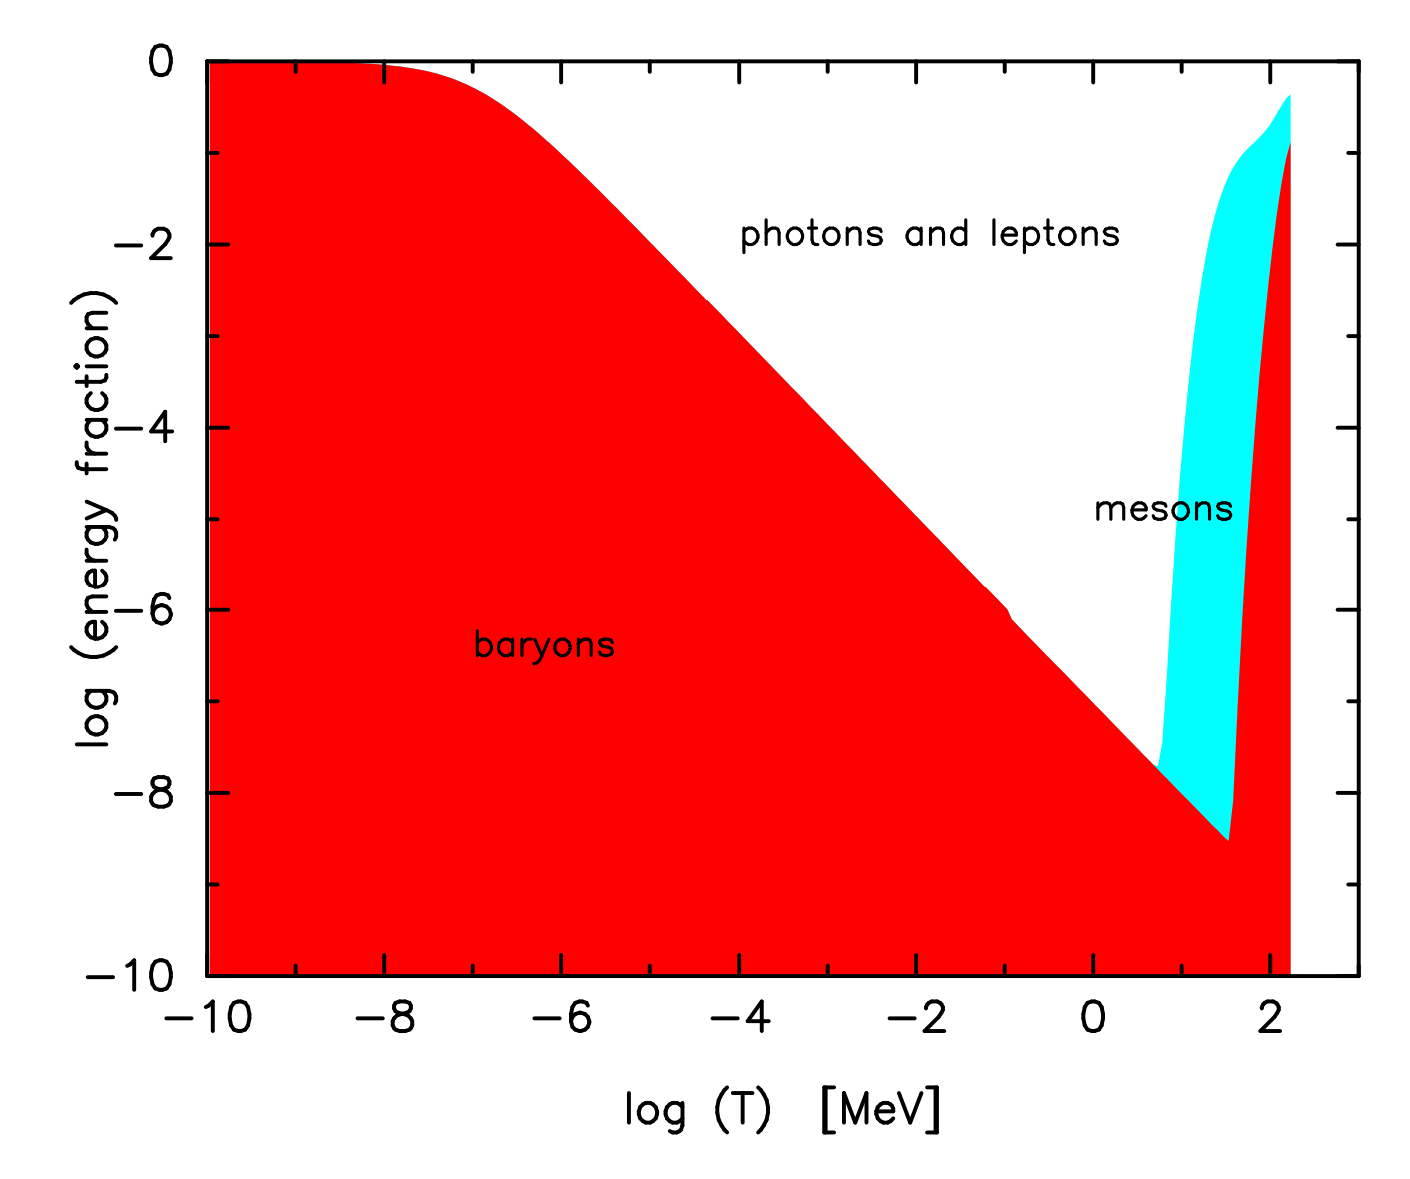
\includegraphics[width=\textwidth]{./plots/hadron_content.png}
\caption{The hadronic content of the luminous Universe as a function of temperature. This figure is a blowup of the right side of \rf{CosmicFraction}. (2003 unpublished, Fromerth \& Rafelski) \cite{Rafelski:2019twp}}
\label{hadron_content}
%\end{center}
\end{figure}
%%%%%%%%%%%%%%%%%%%%%%%%%%%%%%%%%%%%%%%

In \rf{hadron_content}, we present the fraction of visible radiation and matter split between the baryons, mesons, and light and leptons. For a brief period in the early Universe, the hadrons contribution to the energy density of the universe dwarfed that of radiation and leptons \cite{Rafelski:2019twp}. This circumstance would not be true again until the late universe after recombination though by that point dark matter would become the dominant form of matter in the cosmos.

The chemical potential of baryons can be determined by the conserved baryon-per-entropy ratio in adiabatic universe expansion. Considering the net baryon density in early Universe with temperature range $150\,\mathrm{MeV}>T>5\MeV$ \cite{Yang:2021bko}:
\begin{align}\label{Baryon_ChemicalPotential}
\frac{\left(n_B-n_{\overline{B}}\right)}{s}&=\frac{1}{s}\left[\left(n_p-n_{\overline{p}}\right)+\left(n_n-n_{\overline{n}}\right)+\left(n_Y-n_{\overline{Y}}\right)\right]\notag\\
&=\frac{45}{2\pi^4g^s_\ast}\sinh\left[\frac{\mu_B}{T}\right]F_N\left[1+\frac{F_Y}{F_N}\sqrt{\frac{1+e^{-\mu_B/T}\,F_Y/F_K}{1+e^{\mu_B/T}\,F_Y/F_K}}\right].
\end{align}
where we employ the phase-space function $F_i$ for sets of nucleon $N$, kaon $K$, and hyperon $Y$ particles defined in Ref.\,\cite{Letessier:2002ony}, Section 11.4.
\begin{align}
&F_N=\sum_{N_i}\,g_{N_i}W(m_{N_i}/T)\;, \quad N_i=n, p, \Delta(1232),\\
&F_K=\sum_{K_i}\,g_{K_i}W(m_{K_i}/T)\;, \quad K_i=K^0, \overline{K^0}, K^\pm, K^\ast(892),\\
&F_Y=\sum_{Y_i}\,g_{Y_i}W(m_{Y_i}/T)\;, \quad Y_i=\Lambda, \Sigma^0,\Sigma^\pm, \Sigma(1385),
\end{align}
where $g_{N_i,K_i,Y_i}$ are the degenerate factors, $W(x)=x^2K^\mathrm{B}_2(x)$ with $K^\mathrm{B}_2$ is the modified Bessel functions of integer order "$2$". The baryon-per-entropy-ratio can be obtained from present-day measurement of $\left(n_B-n_{\overline{B}}\right)/n_\gamma$, and we obtain: \cite{Yang:2021bko}:
\begin{align}\label{BdS}
\frac{n_B-n_{\overline{B}}}{s}= \left.\frac{n_B-n_{\overline{B}}}{s}\right|_{t_0}=(0.865\pm0.008)\times10^{-10} \;,
\end{align}
The value can be obtained by given $\left(n_B-n_{\overline{B}}\right)/n_\gamma= (0.609\pm0.06)\times10^{-9}$, as well as the entropy per particle for a massless boson $\sigma/n|_\mathrm{boson}\approx 3.60$ and massless fermion $\sigma/n|_\mathrm{fermion}\approx 4.20$.

 Considering the inventory of the Universe strange mesons and baryons, we have reevaluated the temperature of the baryon disappearance.
In Fig. \ref{Baryon_fig} we solve Eq.(\ref{Baryon_ChemicalPotential}) numerically and plot the baryon(antibaryon) number density as a function of temperature in the range $150\,\mathrm{MeV}>T>5\,\mathrm{MeV}$. The temperature where antibaryons disappear from the Universe inventory can be defined when the ratio $n_{\overline B}/(n_B-n_{\overline B})=1$. This condition is reached in an expanding Universe at $T=38.2$\,MeV(vertical black dotted line) which is agree with qualitatively results in Ref.\,\cite{kolb1981early} . 

The antibaryon disappearance temperature does not depend on the baryon and lepton number neutrality $L=B$, it only depends on the baryon-per-entropy ratio assumed to be constant during Universe evolution. The assumption of comoving baryon number conservation is justified by the wealth of particle physics experiments, and the comoving entropy conservation in an adiabatic evolving Universe is a common assumption.
%~~~~~~~Figure~~~~~~~~~~~~~~~~~~~~~~~~~~~~~~~~~~~~~~~~~~~~~~~~~~~
\begin{figure} [ht]
%\begin{center}
\centering
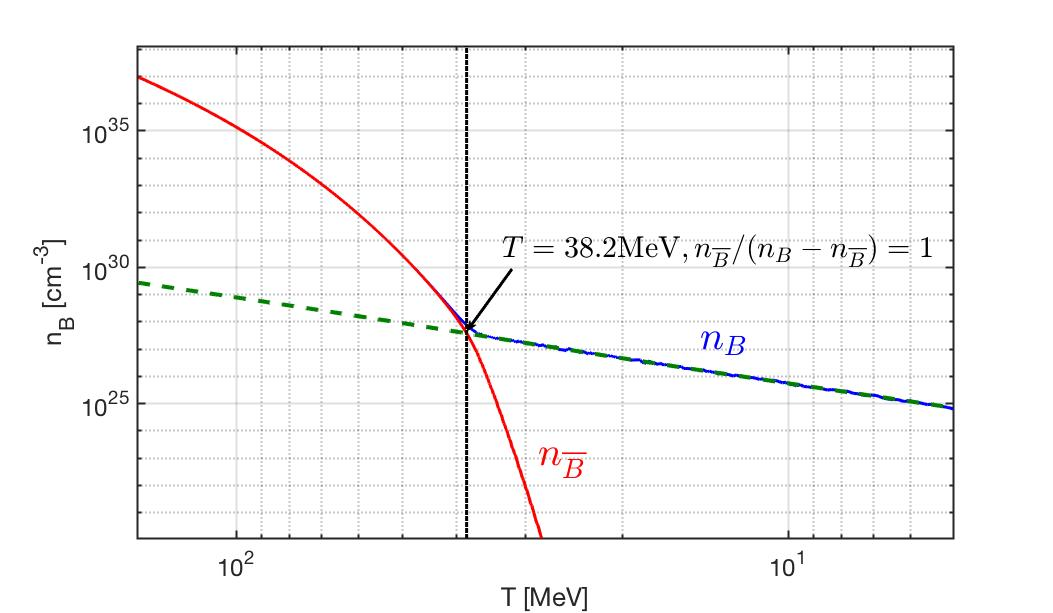
\includegraphics[width=\textwidth]{./plots/Baryon_Antibaryon_cm.jpg}
\caption{The baryon(antibaryon) number density as a function of temperature in the range $150\,\mathrm{MeV}>T>5\,\mathrm{MeV}$. The blue solid line is the baryon density, the red solid line is the antibaryon density. The black dotted line represents $T=38.2$ MeV when the ratio $n_{\overline B}/(n_B-n_{\overline B})=1$ which deifne the condition where $n_{\overline B} $ disappear from the Universe. The temperature we reevaluated  is agree with the results in Ref.\,\cite{kolb1981early} }
\label{Baryon_fig}
%\end{center}
\end{figure}
%~~~~~~~~~~~~~~~~~~~~~~~~~~~~~~~~~~~~~~~~~~~~






%%%%%%%%%%%%%%%%%%%%%%%%%%%%%%%%%%%%%%%%%%%%%%%%%%%%%%%%%%%%
\subsection{Cosmological Strangeness Abundance}\label{sec:Strangeness}
\noindent 
As energy contained in the quark-gluon plasma is used up to create matter and antimatter particles, the high abundance of strange quark pairs present in the plasma is preserved as exotic forms containing strange particles. After hadronization, both charm quarks and strange quarks can form heavy mesons. With time strangeness and charmness decays as they are heavier than the usual quarks and antiquarks. However, unlike charm which disappears from the particle inventory quickly, strangeness can still persist \cite{Yang:2021bko} in the Universe until $T\approx\mathcal{O}(10\mathrm{MeV})$.

We illustrate this by considering an unstable strange particle $S$ decaying into two particles $1$ and $2$ which themselves have no strangeness content. In a dense and high-temperature plasma with particles $1$ and $2$ in thermal equilibrium, the inverse reaction populates the system with particle $S$. This is written schematically as
\begin{align}
 S\Longleftrightarrow1+2,\qquad \mathrm{Example}: K^0\Longleftrightarrow\pi\pi
\end{align}
The natural decay of the particles concerned provides also the intrinsic strength of the inverse, strangeness production reaction. As long as both decay and production reactions are possible, particle $S$ abundance remains in thermal equilibrium. This balance between production and decay rates is called detailed balance. The thermal reaction rate per time and volume for two body-to-one particle reactions $1+2\rightarrow 3$ has been presented before~\cite{Kuznetsova:2008jt,Kuznetsova:2010pi}. In full kinetic and chemical equilibrium, the reaction rate per time per volume is given by~\cite{Kuznetsova:2010pi} :
\begin{align}
&R_{12\to 3}=\frac{g_3}{(2\pi)^2}\,\frac{m_3}{\tau^0_3}\,\int^\infty_0\frac{p^2_3dp_3}{E_3}\frac{e^{E_3/T}}{e^{E_3/T}\pm1}\Phi(p_3)\;,
\end{align}
where $\tau^0_3$ is the vacuum lifetime of particle $3$. The positive sign $``+"$ is for the case when particle $3$ is a boson, and negative sign $``-"$ for fermion. The function $\Phi(p_3)$ for the non-relativistic limit $m_3\gg p_3,T$ can be written as 
\begin{align}
\Phi(p_3\to0)=2\frac{1}{(e^{E_1/T}\pm1)(e^{E_2/T}\pm1)}.
\end{align}


When the back reactions are faster than the Universe expansion, which condition(s) we characterize in the following, we can explore the Universe composition assuming both kinetic and particle abundance equilibrium (chemical equilibrium). In Fig.~\ref{EquilibPartRatiosFig} we solve the chemical potential of strangeness numerically anf show the chemical equilibrium particle abundance ratios of the composition of hadronic Universe \cite{Yang:2021bko}. We have
\begin{itemize}
\item
In the temperature range $150\,\mathrm{MeV} >T >40$\,MeV the Universe is rich in physics phenomena involving strange mesons, (anti)baryons including (anti)hyperon abundances. Pions $\pi(q\bar q)$ are the most abundant hadrons because of their low mass and the inverse decay reaction $\gamma\gamma\rightarrow\pi^0$, which assures chemical equilibrium~\cite{Kuznetsova:2008jt}. It is important to realize that hadrons always are a part of the evolving Universe, a point not much discussed in literature.

\item
For temperature $150\,\mathrm{MeV}>T>20\,\mathrm{MeV}$ the Universe is meson-dominant and the strangeness is dominantly present in the meson sector with $s=\bar s$. For temperature $T<20$\,MeV, the Universe becomes baryon-dominant. Below temperature $T<13$\,MeV, strangeness is present dominantly in hyperons, we have $(s -\bar s)\ne 0$.
\end{itemize}
%~~~~~~~~~~~~~~~~~~~~~~~~~~~~~~~~~~~~~~~~~~~~~~~~~~~~~~~~~~~~~~~~~~~~~~~~~~~~~~~~
\begin{figure}[bt]
%\begin{center}
\centering
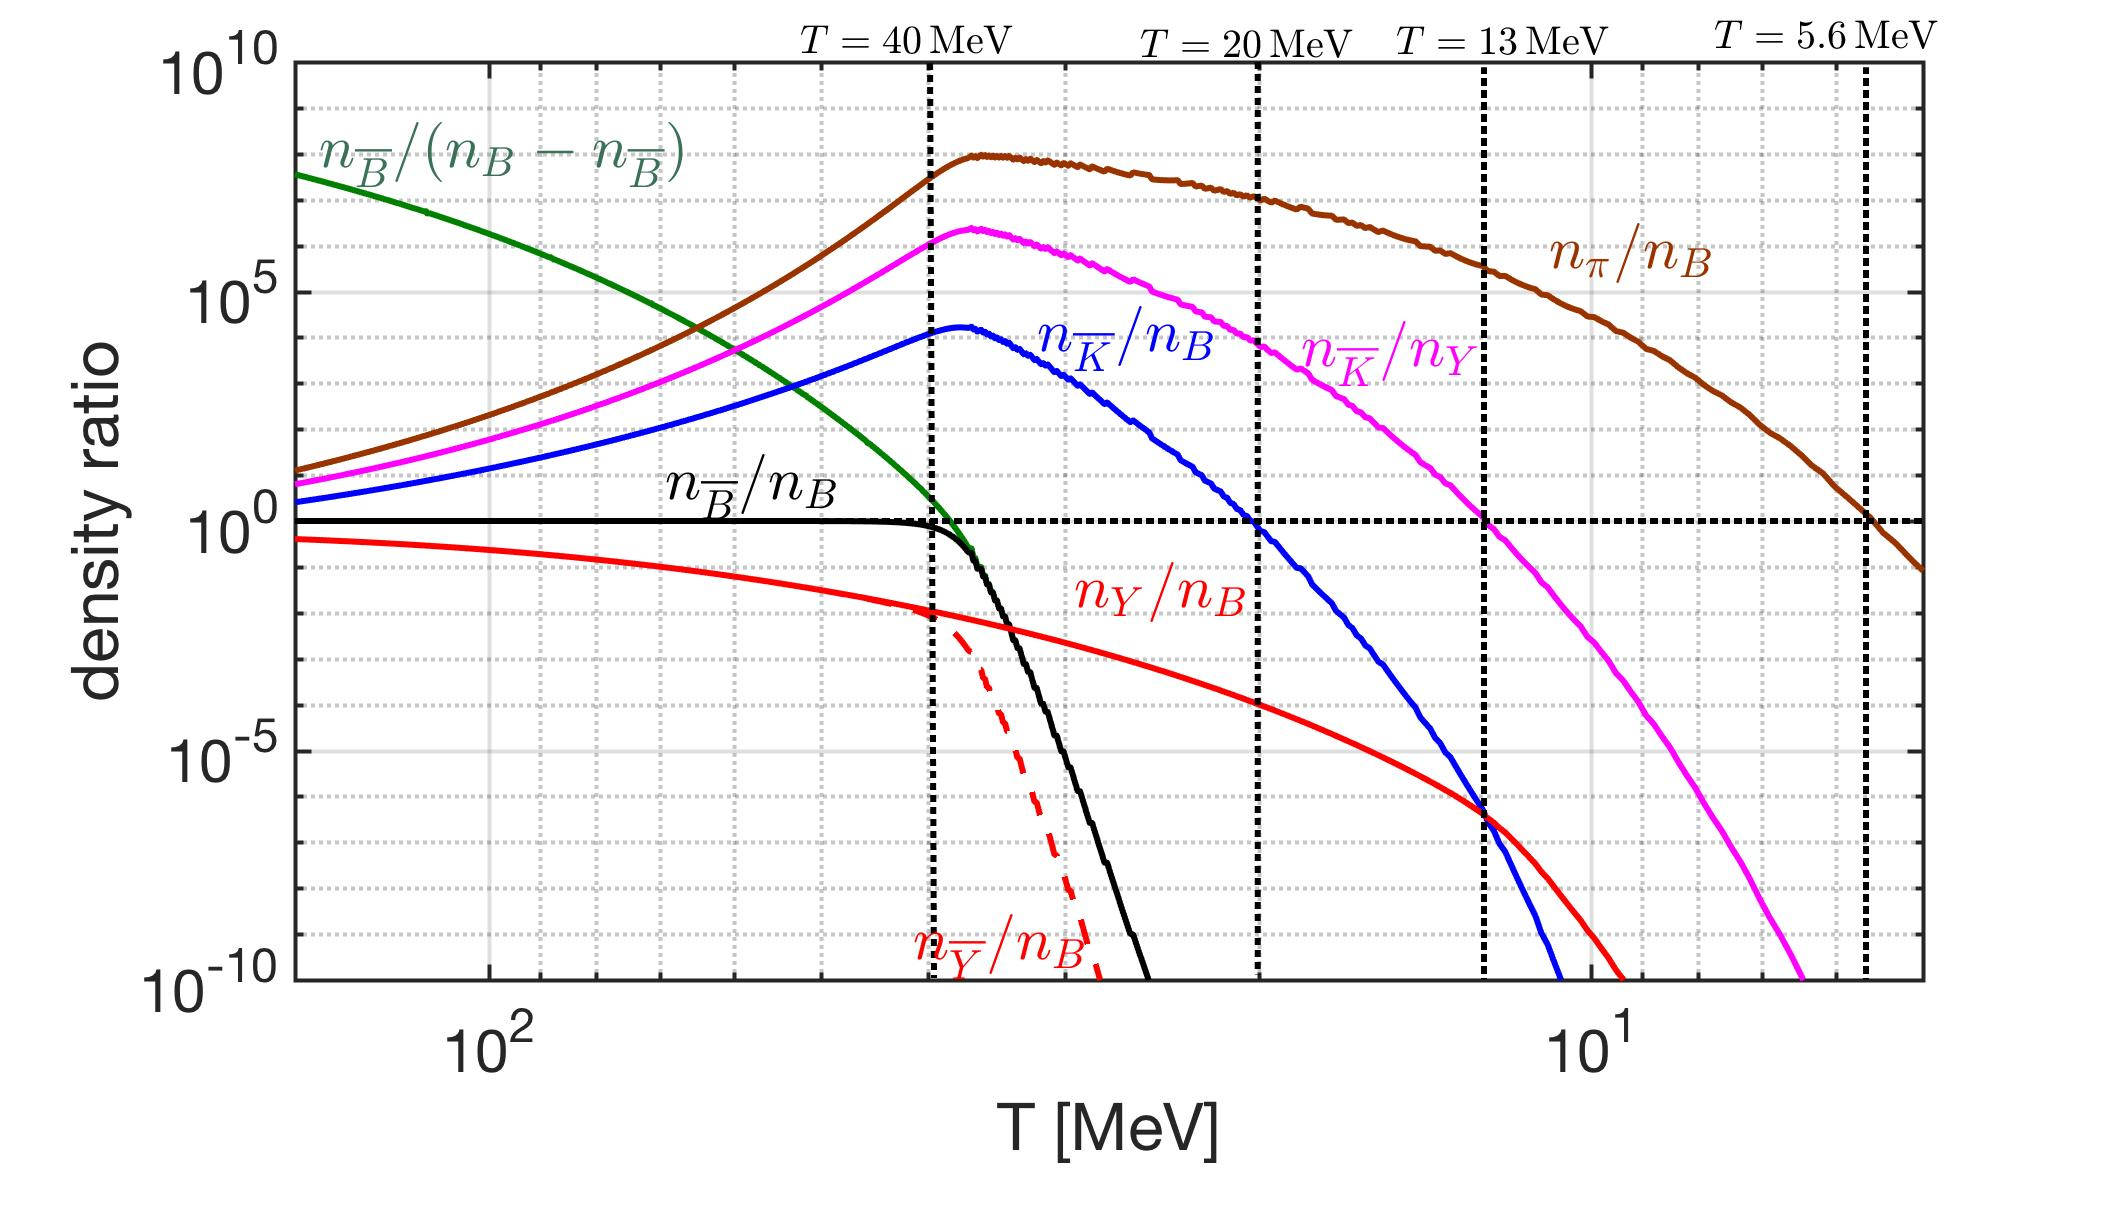
\includegraphics[width=\textwidth]{./plots/Meson_Baryon_density_ratio_CTYang.jpg}
\caption{Ratios of hadronic particle number densities as a function of temperature $150\,\mathrm{MeV}> T>10\,\mathrm{MeV}$ in the early Universe with baryon $B$ yields: pions $\pi$ (brown line), kaons $K( q\bar s)$ (blue), antibaryon $\overline B$ (black), hyperon $Y$ (red) and anti-hyperons $\overline Y$ (dashed red). Also shown $\overline K/Y$(purple).}
\label{EquilibPartRatiosFig}
%\end{center}
\end{figure}
%~~~~~~~~~~~~~~~~~~~~~~~~~~~~~~~~~~~~~~~~~~~~~~~~~~~~~~~~~~~~~~~~~~~~~~~~~~~~~
In Fig.~\ref{Strangeness_map2} we shows important source reactions for  strange quark abundance in baryons and mesons, considering both open and hidden strangeness ($s\bar s$-content). The important reactions are $l^-+l^+\rightarrow\phi$, $\rho+\pi\rightarrow\phi$, $\pi+\pi\rightarrow K_\mathrm{S}$, $\Lambda \leftrightarrow \pi+ N$, and $\mu^\pm+\nu\rightarrow K^\pm$. Muons and pions are coupled through electromagnetic reactions $\mu^++\mu^-\leftrightarrow\gamma+\gamma$ and $\pi^0\leftrightarrow\gamma+\gamma$ to the photon background and retain their chemical equilibrium respectively~\cite{Rafelski:2021aey,Kuznetsova:2008jt}. The large $\phi\leftrightarrow K+K$ rate assures $\phi$ and $K$ are in relative chemical equilibrium. 
%~~~~~~~Figure~~~~~~~~~~~~~~~~~~~~~~~~~~~~~~~~~~~~~~~~~~~~~~~~~~~~~~~~~~~~~~~~~~~~
\begin{figure} %[ht]
%\begin{center}
\centering
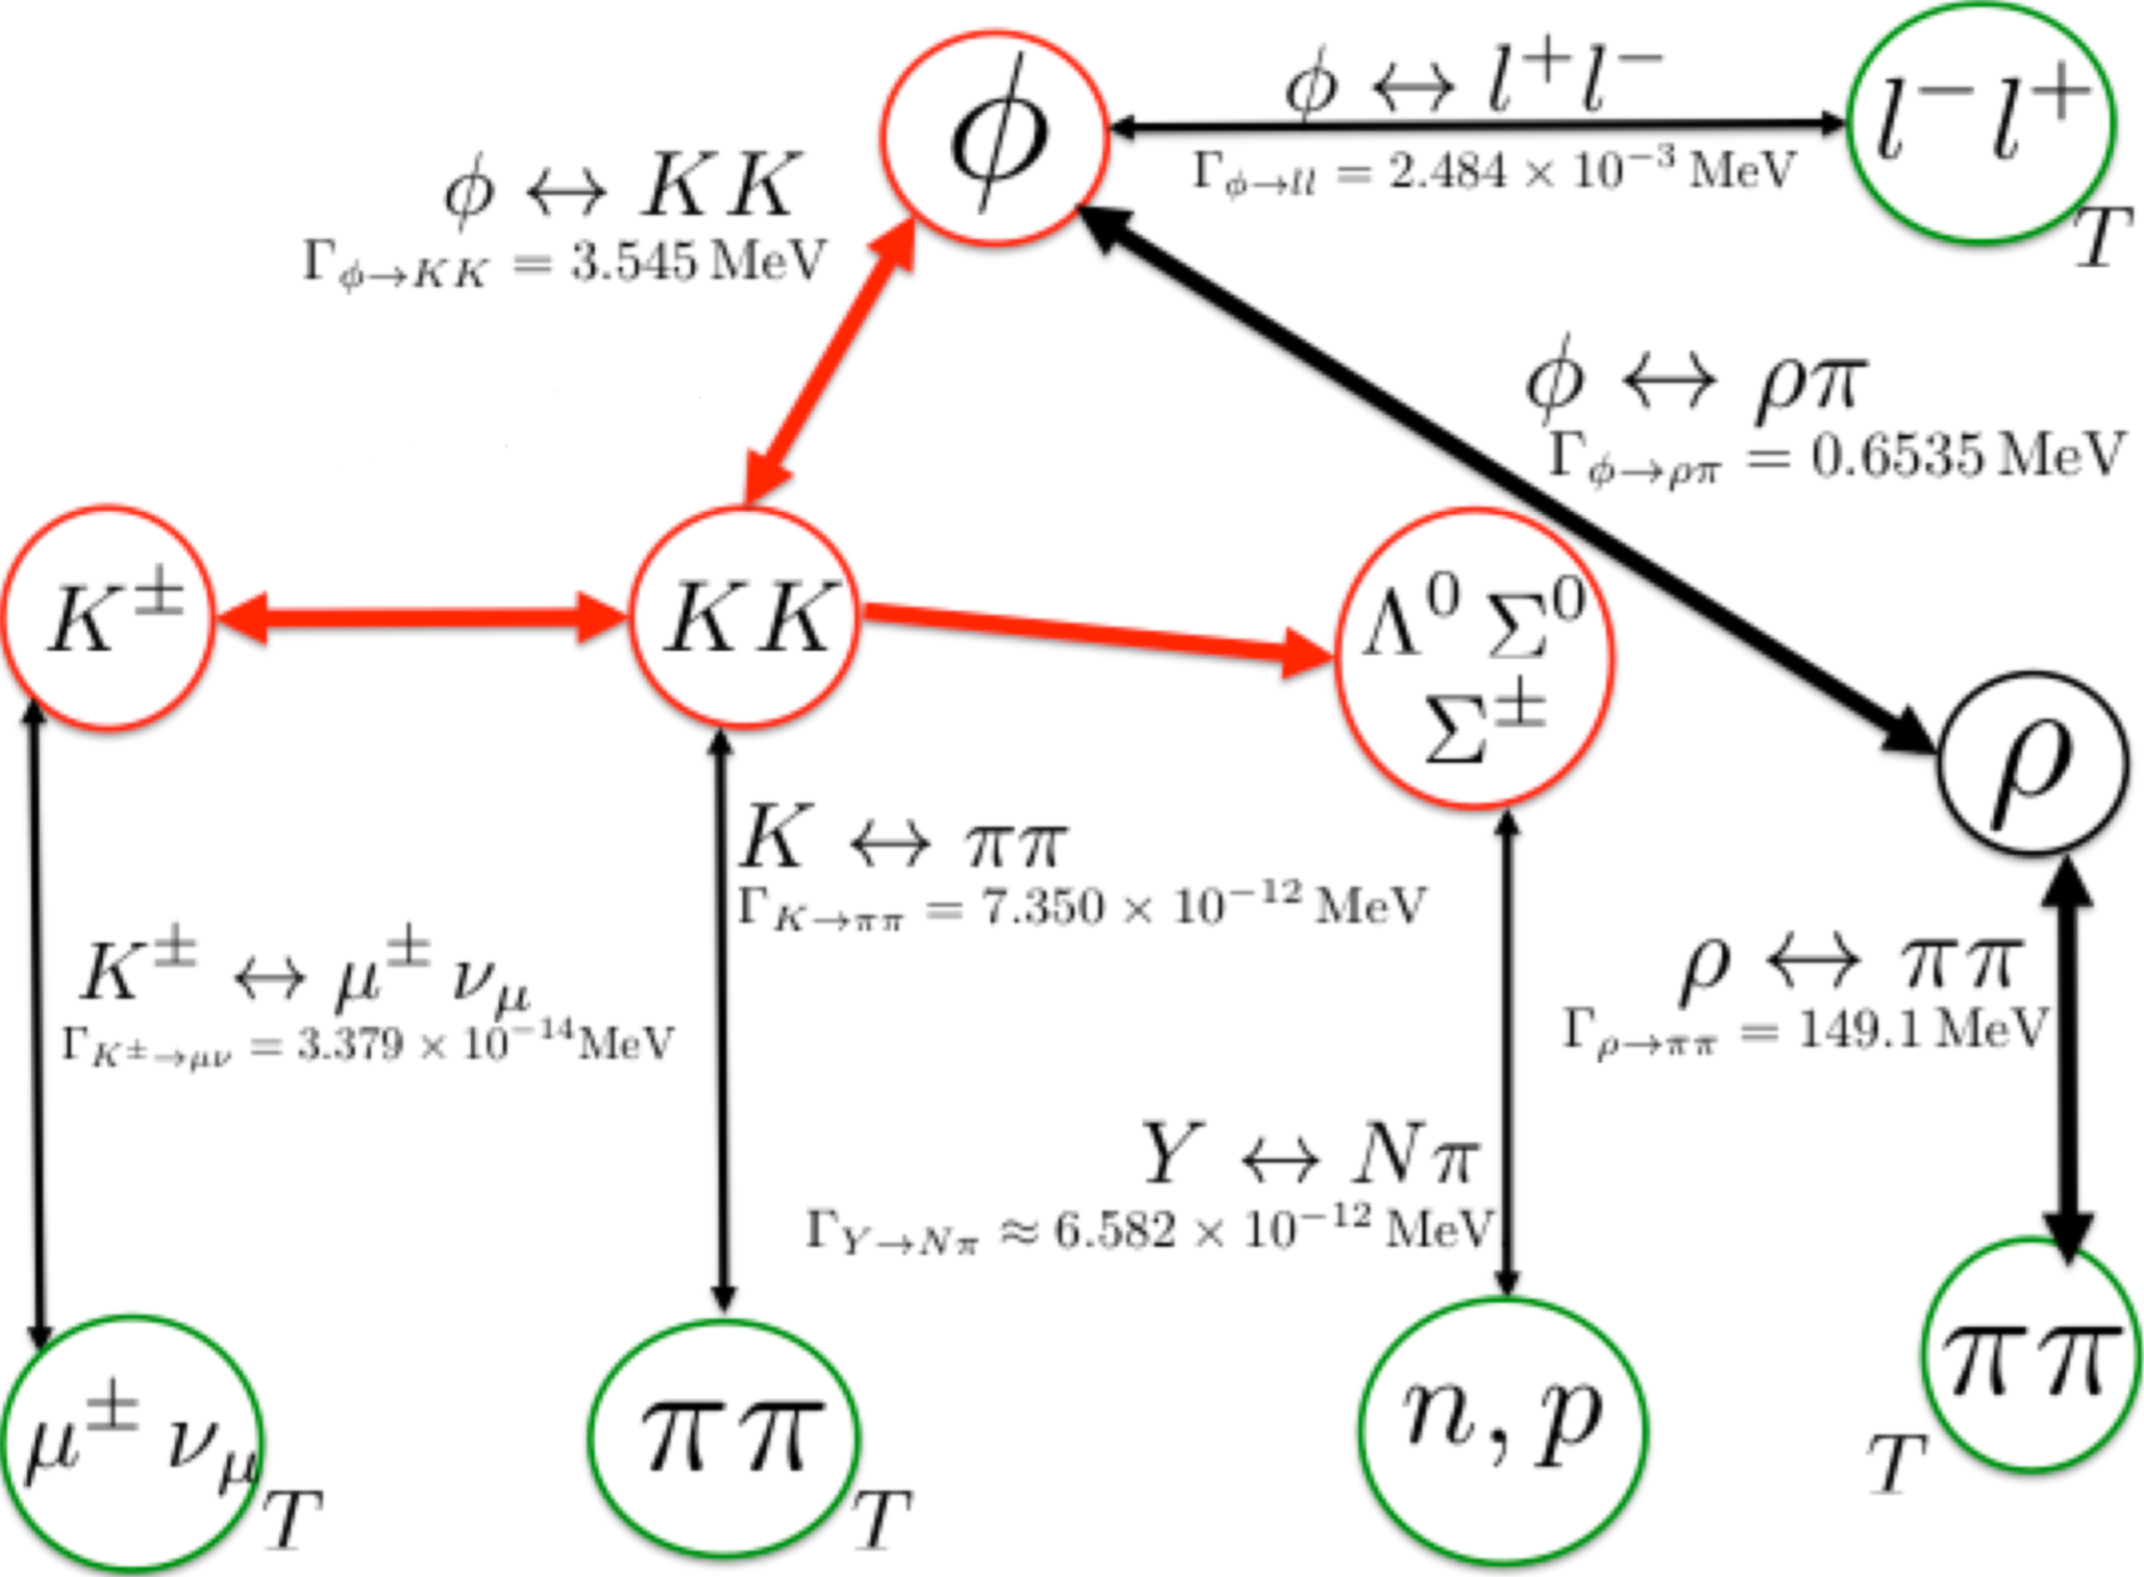
\includegraphics[width=0.8\linewidth]{./plots/Strangeness002_new.pdf}
\caption{
The strangeness abundance of changing reactions in the primordial Universe. The red circles show strangeness carrying hadronic particles; red thick lines denote effectively instantaneous reactions. Black thick lines show relatively strong hadronic reactions.}
\label{Strangeness_map2}
%\end{center}
\end{figure}
%~~~~~~~~~~~~~~~~~~~~~~~~~~~~~~~~~~~~~~~~~~~~~~~~~~~~~~~~~~~~~~~~~~~~~~~~~~
%~~~~~~~Figure~~~~~~~~~~~~~~~~~~~~~~~~~~~~~~~~~~~~~~~~~~~~~~~~~~~~~~~~~~~~~~~~~~~~~~~~~~
\begin{figure}[ht]
%\begin{center}
\centering
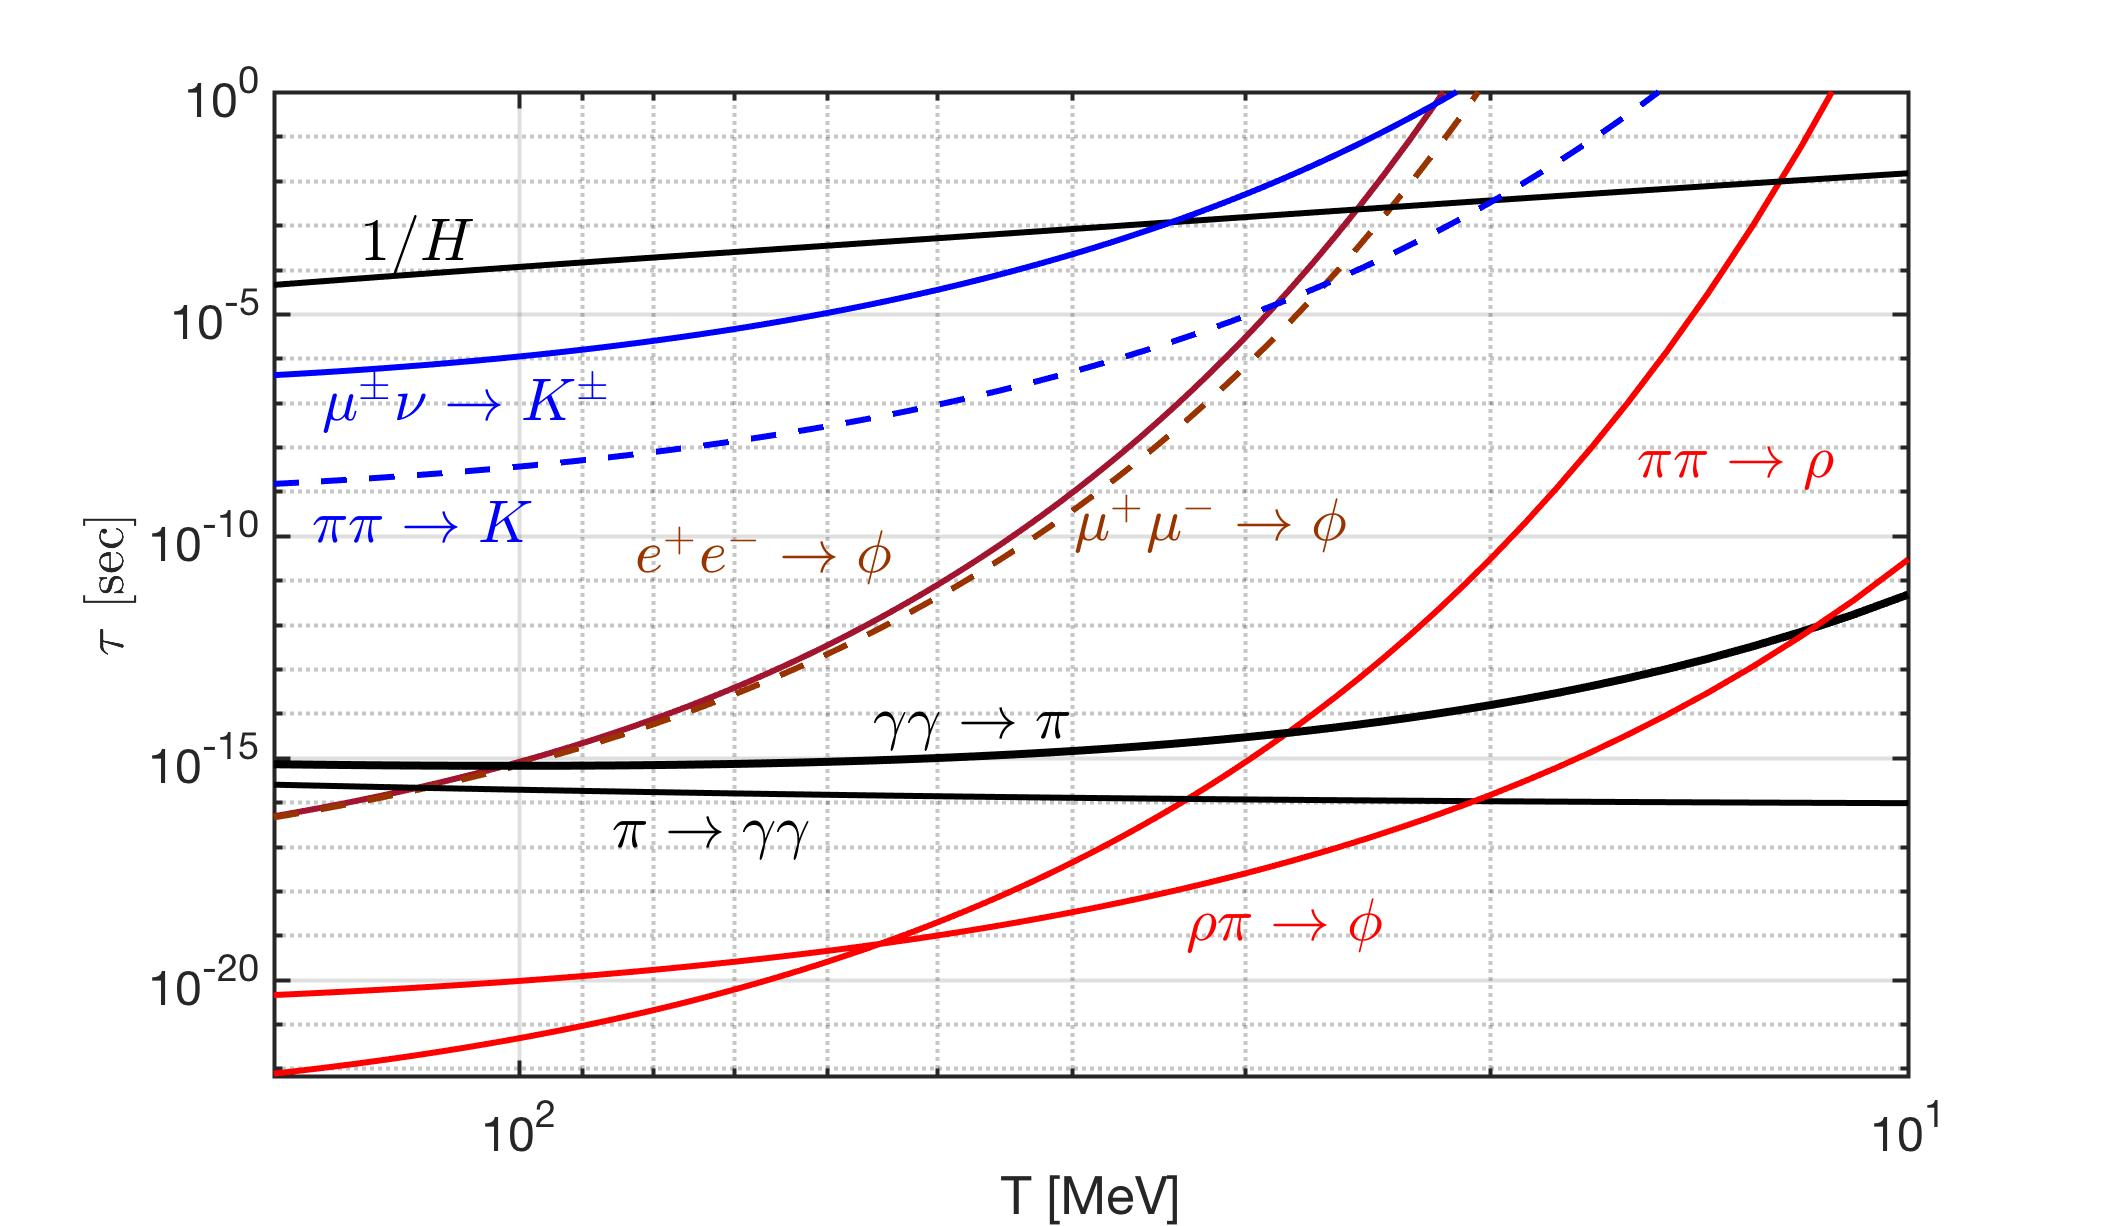
\includegraphics[width=1.0\linewidth]{./plots/Strangeness_Hubble_CTYang_V2.jpg}
\caption{The hadronic relaxation reaction times in meson sector as a function of temperature $T$, are compared to Hubble time $1/H$ (black solid line). At the bottom, the horizontal black-dashed line is the natural (vacuum) lifespan of $\rho$.}
\label{reaction_time_tot}
%\end{center}
\end{figure}
%~~~~~~~~~~~~~~~~~~~~~~~~~~~~~~~~~~~~~~~~~~~~~~~~~~~~~~~~~~~~~~~~~~~~~~~~~~~~~~~~~~~~~
Once the primordial Universe expansion rate, given as the inverse of the Hubble parameter $1/H$, overwhelms the strongly temperature-dependent back-reaction, the decay $S\rightarrow 1+2$ occurs out of balance and particle $S$ disappears from the Universe. In order to determine where exactly strangeness disappears from the Universe inventory we explore the magnitudes of a relatively large number of different rates of production and decay processes, and compare these with the Hubble time constant \cite{{Yang:2021bko}}. We have
\begin{itemize}
\item \textbf{Strangeness in meson era:}
The relevant interaction rates competing with Hubble time involving strongly interacting mesons are the reactions $\pi+\pi\leftrightarrow K$, $\mu^\pm+\nu\rightarrow K^\pm$, $l^++l^-\rightarrow\phi$, $\rho+\pi\leftrightarrow\phi$, and $\pi+\pi\leftrightarrow\rho$. 
 These relaxation time $\tau$  are compared with Hubble time in Fig.~\ref{reaction_time_tot}. In Table\,\ref{FreezeoutTemperature_table} we show the characteristic strangeness reactions and their freezeout temperatures in the early Universe. 
\\
It shows that once the reactions freezout from the cosmic plasma, the corresponding detailed balance is broken and the inverse decay reactions are acting like a "hole" in the strangeness abundance "pot”.
The first freezeout reaction is the weak interaction $\mu^\pm+\nu_{\mu}\rightarrow K^\pm$ at $T_f^{K^\pm}=33.8\,\mathrm{MeV}$, and followed by the electromagnetic process $l^-+l^+\rightarrow\phi$ at $T_f^\phi=23\sim25\,\mathrm{MeV}$. At $T_f^K=19.8\,\mathrm{MeV}$ the hadronic reaction $\pi+\pi\rightarrow K$ becomes slower than the Hubble expansion. The reactions $\gamma+\gamma\rightarrow\pi$ and $\rho+\pi\leftrightarrow\phi$ are faster compared to $1/H$. However, the $\rho\to\pi+\pi$ lifetime (black dashed line in Fig.~\ref{reaction_time_tot}) is faster than the reaction $\rho+\pi\leftrightarrow\phi$; Hence most of $\rho$-meson decays faster and cannot contribute to the strangeness creation in the meson sector. Below the temperature $T<20$\,MeV, all the detail balances in the strange meson reactions are broken and the strangeness in the meson sector should disappear rapidly, were it not for the small number of baryons present in the Universe.
%~~~~~~~~~~~table~~~~~~~~~~~~~~~~~~~~~~~~~~~~~~~~~~~~~~~~~~~~~~~~~~~~~~~~~~~~~~~~~~~~~~~~~~~~~~
\begin{table}%[ht]
\caption{The characteristic strangeness reaction and their freezeout temperature and temperature width in early Universe.}
\label{FreezeoutTemperature_table} 
\centering
\begin{tabular}{c| c| c}
\hline\hline
Reactions &Freezeout Temperature (MeV) & {$\Delta T_f$\,(MeV)} \\
\hline
$\mu^\pm\nu\rightarrow K^\pm$ & $T_f=33.8$\,MeV & {$3.5$ \,MeV}\\ 
\hline
$e^+e^-\rightarrow \phi$ & $T_f=24.9$\,MeV &{$0.6$\,MeV}\\
$\mu^+\mu^-\rightarrow\phi$ & $T_f=23.5$\,MeV &{$0.6$\,MeV}\\
\hline
 $\pi\pi\rightarrow K$ & $T_f=19.8$\,MeV&{$1.2$\,MeV}\\
\hline
$\pi\pi\rightarrow\rho$ & $T_f=12.3$\,MeV&{$0.2$\,MeV}\\
\hline\hline
\end{tabular}
\end{table}

%~~~~~~~~~~~~~~~~~~~~~~~~~~~~~~~~~~~~~~~~~~~~~~~~~~~~~~~~~~~~~~~~~~~~~~~~~ 


\item \textbf{Strangeness in hyperons era:}
In order to understand strangeness in hyperons, we evaluated the reaction $\pi +N\rightarrow K+\Lambda$, the strangeness exchange reaction $\overline{K}+N\rightarrow \Lambda+\pi$, and the strangeness decay $\Lambda\rightarrow N+\pi$, in detail. The general form for thermal reaction rate per volume is discussed in~\cite{Letessier:2002ony} (Eq.(17.16), Chapter 17). In Fig.~\ref{Lambda_Rate_volume.fig} we saw that for $T<20$\,MeV, the reactions for the hyperon $\Lambda$ production is dominated by $\overline{K}+N\leftrightarrow\Lambda+\pi$. Both strangeness and anti-strangeness disappear from the Universe via the reactions $\Lambda\rightarrow N+\pi$ and $K\to\pi+\pi$, keeping the $s=\bar s$. Beginning with $T=12.9$ MeV, the dominant reaction is $\Lambda\leftrightarrow N+\pi$, which shows that at a lower temperature we still have (very little) strangeness remnant in the $\Lambda$. In this case, the strangeness abundance becomes asymmetric and we have $s\gg\bar{s}$ in the early Universe. Hence, strange hyperons and anti hyperons could enter into dynamic nonequilibrium condition including $\langle s-\bar s\rangle \ne 0$.


%~~~~~~~~~~~~~~~~~~~~~~~~~~~~~~~~~~~~~~~~~~~~~~~~~~~~~~~~~~~~~~~~~~~~~~~~~~~~~~~~
\begin{figure}[ht]
\begin{center}
\centering
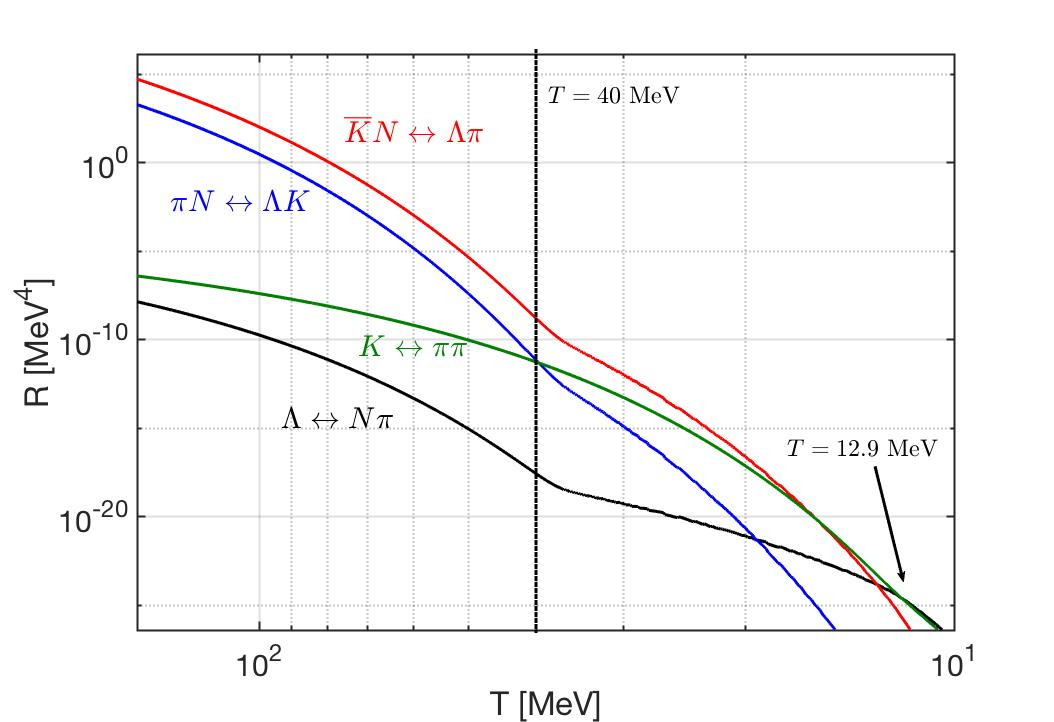
\includegraphics[width=0.8\linewidth]{./plots/NewHyperonRate_CTYang.jpg}
\caption{Thermal reaction rate $R$ per volume and time for important hadronic strangeness production and exchange processes as a function of temperature $150\,\mathrm{MeV}> T>10\,\mathrm{MeV}$ in the early Universe.}
\label{Lambda_Rate_volume.fig}
\end{center}
\end{figure}
%~~~~~~~~~~~~~~~~~~~~~~~~~~~~~~~~~~~~~~~~~~~~~~~~~~~~~~~~~~~~~~~~~~~~~~~~~~~~~~
\end{itemize}
The primary conclusion of the study of strangeness production and content in the early Universe, following on QGP hadronization, is that the relevant temperature domains indicate a complex interplay between baryon and meson (strange and non-strange) abundances and non-trivial decoupling from equilibrium for strange and non-strange mesons.



\subsection{Pion Abundance in the Early Universe}\label{sec:Pions}
\noindent 
In early universe, the $\pi^0$ vacuum life span $\tau_{\pi^0}^0=(8.52\pm0.18)\times10^{-17} {\rm sec}$ is rather short compare to the Hubble expansion time $1/H=(10^{-3}\sim10^{-4})$ sec. In this case, one is tempted to presume that the decay process dominates and $\pi^0$ disappears in early Universe. However, there must be a detailed balance in the thermal bath: the production process in a suitable environment must be able to form $\pi^0$ with strength corresponding to the decay process lifespan. 

In general, $\pi^0$ in the QED plasma is produced predominantly in the thermal two-photon fusion:
\begin{align}
\gamma+\gamma \rightarrow \pi^{0}. 
\end{align}
These formation processes are the inverse of the decay process of $\pi^0$. The smallness of the electron-formation of $\pi^0$ is characterized by the small  branching ratio in $\pi^0$ decay $B=\Gamma_{ee}/\Gamma_{\gamma\gamma}=6.2\pm 0.5\times10^{-8}$.
For $\pi^{\pm}$ can be produced in $\pi^0\pi^0$ charge exchange scattering:
\begin{align}
\pi^0 + \pi^0 \rightarrow \pi^{+} + \pi^{-}, \qquad\gamma+\gamma \rightarrow \pi^{+} + \pi^{-}, \qquad
e^+ + e^- \rightarrow \pi^{+} + \pi^{-}. 
\end{align}
We find  that for $\pi^{\pm}$ production, the last two processes are much slower compared to the first, in case that $\pi^0$ density is near chemical equilibrium. The general form for invariant production rates and relaxation time is discussed in paper \cite{Kuznetsova:2008jt}, we have for $\gamma\gamma\to\pi^0$
\begin{align}
R_{\gamma\gamma\to\pi^0}=&\int\frac{d^{3}{p_{\pi}}}{(2\pi\ )^32E_{\pi}}
   \int\frac{d^{3} {p_{2\,\gamma}}}{(2\pi\ )^32E_{2\,\gamma}}
   \int\frac{d^{3}{p_{1\,\gamma}}} {(2\pi\ )^32E_{1\,\gamma} }\left(2\pi\right)^{4}
 \delta^{4}\left(p_{1\,\gamma}+p_{2\,\gamma}-p_{\pi}\right)\times \nonumber\\ &
  \sum_{spin}\left|\langle p_{1\,\gamma}p_{2\,\gamma}\left| M\right|p_{\pi}\rangle\right|^{2}
   f_{\pi}(p_{\pi})f_{\gamma}(p_{1\,\gamma})f_{\gamma}(p_{2\,\gamma})
 \Upsilon^{-2}_{\gamma}\Upsilon_{\pi^{0}}^{-1}e^{u \cdot p_{\pi}/T}. \label{pi0pr}
 \end{align}
where $\Upsilon_i$ is the fugacity of particle $i$. For $\pi^\pm$ production, we have
\begin{align}
{R_{1\,2 \leftrightarrow \pi^+\pi^-}} = \frac{g_1g_2}{32\pi^4}\frac{T}{1+I}
\int_{s_{th}}^{\infty}ds\sigma(s)\frac{(s-(m_{1}+m_2)^2)(s-(m_1-m_2)^2)}{\sqrt{s}}K_1(\sqrt{s}/T),
\end{align}
(compared to reference~\cite{Letessier:2002ony} our definition is changed 
$R_{12\rightarrow 34} \rightarrow 
R_{12 \rightarrow 34}/(\Upsilon_1 \Upsilon_2)$)
where $m_1$ and $m_2$, $g_1$ and $g_2$, $\Upsilon_1$ and $\Upsilon_2$ are masses, degeneracy and fugacities of initial interacting particles. 

Fig \ref{taumupi} {\xred Fig. 16 discussion only.} shows the invariant production rates $R$ of pion  for the different processes considered as a function of temperature $T\in [3,50]$ MeV. It shows that $\gamma+\gamma\to \pi^0$(solid blue line) is the dominant mechanism of $\pi^0$ production. The other solid line with dots corresponds to $e^++e^-\to \pi^0$ reaction which in essence remains, in comparison, insignificant. Its importance follows from the fact that it provides the second most dominant path to $\pi_0$ formation at the lowest temperatures considered.
%~~Figure~~~~~~~~~~~~~~~~~~~~~~~~~~~~~~~~~~~~~~~
\begin{figure}[ht]
\centering
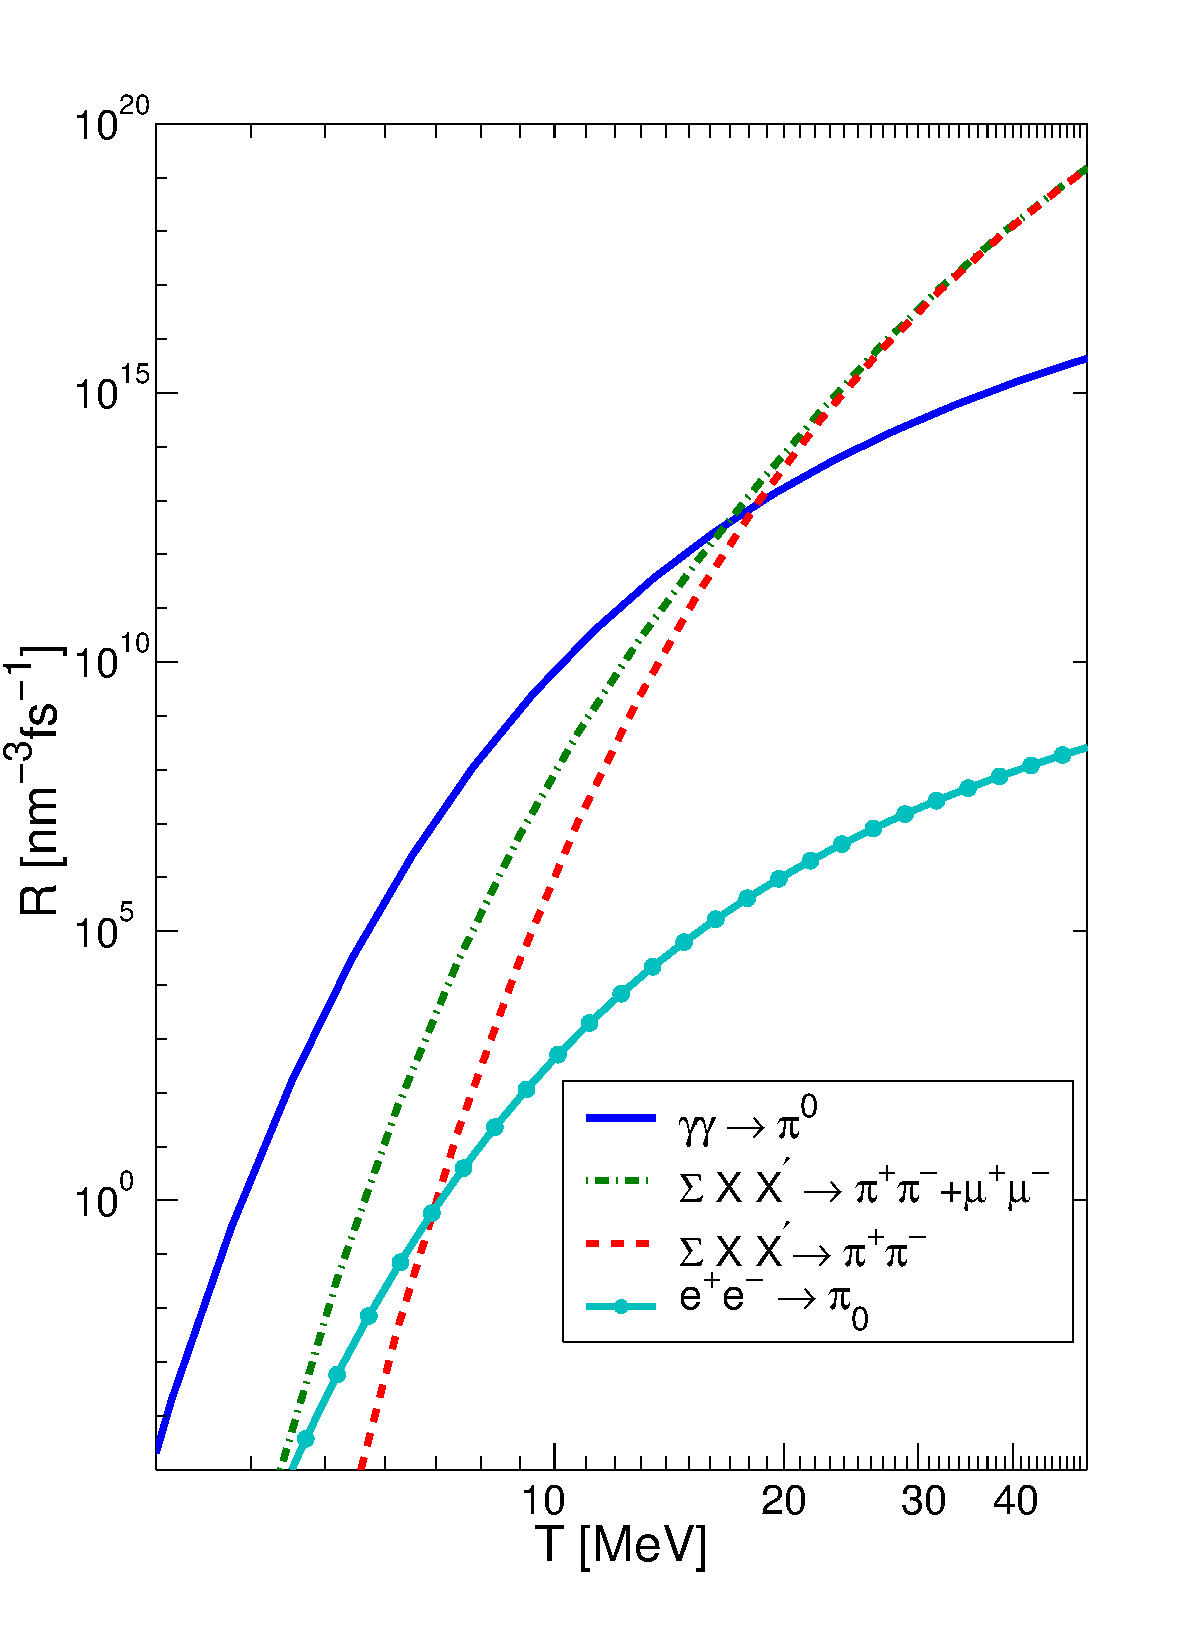
\includegraphics[width=0.6\columnwidth]{./plots/pions1.pdf}
\caption{{\xred Remove figure. Salvage text?} The invariant pion production rates as a function of temperature $T$. The sum of formation rates of charged pion pairs (dashed, red) by all reactions: $\pi^{0}+\pi^{0}\to \pi^{+}+\pi^{-},  \gamma+\gamma \to \pi^{+}+\pi^{-}, e^++e^-\to \pi^{+}+\pi^{-}$.
We also present the sum of all reactions leading to either a charged pion pair, or muon pair (dot-dashed, green) lines with reactions:$\gamma+\gamma \to \mu^{+}+\mu^{-}, e^++e^-\to \mu^{+}+\mu^{-}$. Figure adapted from \cite{Kuznetsova:2008jt}}.
\label{taumupi}
\end{figure}
%~~~~~~~~~~~~~~~~~~~~~~~~~~~~~~~~~~~~~~~~~~~~~~
Since the  $\gamma+\gamma\to \pi^0$ is the dominant mechanism of pion production, then we can ask the question: at what temperature in the expanding early Universe does this reaction
`freeze' out, that is the $\pi^0$ decay overwhelms the production rate and the yield
falls away from chemical equilibrium yield. To answer this question, we study the dynamic equation of $\pi^0$ which describes the evolution of $\pi^0$ number density in early universe \cite{Fromerth:2012fe}. Omitting all sub-dominant processes, the dynamic equation of $\pi^0$ abundance can be written as:
\begin{align}
\frac{d}{dt}\Upsilon_{\pi^0}=\frac{1}{\tau_T}\Upsilon_{\pi^0}+\frac{1}{\tau_s}\Upsilon_{\pi^0}+\frac{1}{\tau_{\pi^0}}\left(\Upsilon^2_\gamma-\Upsilon_{\pi^0}\right)
\end{align}
where $\tau_T$ and $\tau_S$ are the kinematic relaxation time for the evolution of the temperature and entropy, and $\tau^{\pi^0}$ is the chemical relaxation time for $\pi^0$. We have
\begin{align}
\frac{1}{\tau_T}\equiv -T^3g^*\frac{d (n_{\pi}/(\Upsilon_3
g^*T^3))/dT}{dn_{\pi}/d{\Upsilon_3}}{\dot T},\label{tauT} \quad
\frac{1}{\tau_{S}}\equiv
-\frac{n_{\pi}/\Upsilon_3}{dn_{\pi}/d{\Upsilon_3}}\frac{d\ln (g^*VT^3)}{dT}
\dot{T},\quad
\tau_{\pi^0}=\frac{dn_{\pi^0}/d\Upsilon_{\pi^0}}{R_{\pi^0}} 
\end{align}
Where $n_{\pi^0}$ is the number density of pion and we introduced the minus sign above in order to have $\tau_T$, $\tau_S>0$. Entropy is conserved in the expanding Universe, and in the radiation-dominated Universe we have $d(T^3V)/dT=0$, and hence $1/\tau_S=0$. The effect of universe expansion and dilution of number density is described by $1/\tau_T$. Comparing $\tau_T$ to the chemical relaxation time $\tau_{\pi^0}$ can provide the quantitative condition for freezeout from chemical equilibrium. In the case, of massive pion $m_{\pi}\gg T$, we have \cite{Kuznetsova:2009xh}
\begin{align}
\tau_T\approx\frac{T}{m_{\pi}H}.
\end{align}
 In Fig.(\ref{reaction_time_tot}) {\xred Fig. 16 discussion only.} we compare the relaxation time of $\tau_{\pi^0}$ to the Hubble time $1/H$, it shows that $\tau_{\pi^0}\ll 1/H$. In such a case, the yield of $\pi^0$ is expected to be chemical equilibrium. Since the decay rate is compensated by the production rate, and within $100$ the chemical equilibrium yield is attained even as its thermal number density gradually decreases. This phenomenon can be attributed to the high population of photons. In such an environment, it remains probable to find high-energy photons to fuse into $\pi^0$ in the early universe. 

%%%%%%%%%%%%%%%%%%%%%%%%%%%%%%%%%%%%%%%
\section{Leptonic Epoch} \label{sec:Leptonic}
\subsection{Thermal Degrees of Freedom}\label{sec:Freedom}
\noindent The leptonic epoch dominated by photons and both charged and neutral leptons is notable for being the last time where neutrinos played an active role in the Universe's thermal dynamics before decoupling and becoming free-streaming. In the early stage of this plasma after the hadronization era ended $T\approx\mathcal{O}(10\MeV)$, neutrinos represented the highest energy density followed by the light charged leptons and then finally the photons. The differing energy densities were related by
\begin{align}
\rho_{e^{\pm}}\approx\left(2\times\frac{7}{8}\right)\rho_{\gamma}\,,\qquad\rho_{\nu}\approx\left(3\times\frac{7}{8}\right)\rho_{\gamma}\,.
\end{align}
The reason for this hierarchy is because of the degrees of freedom \cite{Coleman:2003hs,Rafelski:2013yka} available in each species in thermal equilibrium. The factor of $7/8$ arises from the difference in pressure contribution from bosons versus fermions \cite{Rafelski:2013yka}. While photons only exhibit two helicity degrees of freedom, the charged light leptons could manifest as both matter (electrons), antimatter (positrons) and as well as two helicities yielding $2\times2=4$. The neutral leptons made up of the neutrinos however had three thermally active species $3\times2=6$ boosting their energy density in that period to more than any other contribution. The muon-antimuon energy density was also controlled by its degrees of freedom matching that of $e^{\pm}$ until $T\approx100\GeV$ when the heavier lepton no longer satisfied the ultra-relativistic (and thus massless) limit. This separation of the two lighter charge lepton dynamics is seen in \rf{CosmicFraction} after hadronization.

The measured degrees of freedom also adds a constraint on the question whether neutrinos are Dirac or Majorana particles. If neutrinos are Dirac-like and have right-handed components, then it is necessary these fields do not become sufficiently populated thermally during this epoch as it would drive the neutrino effective degrees of freedom $N^{\nu}_{\mathrm{eff}}$ away from three. The presence of sterile neutrinos could also inflate $N_{\mathrm{eff}}^{\nu}$ during this epoch for the same reasoning \cite{Kopp:2011qd,Hamann:2011ge,Kopp:2013vaa,Lello:2014yha,Birrell:2014qna} or have a connection to dark matter \cite{Weinberg:2013kea,Giusarma:2014zza}. The neutrino degrees of freedom will be more fully discussed in \rsec{sec:EffectiveNeutrino}.

\subsection{Muon Abundance in the Early Universe} \label{sec:Muons}
\noindent Muon abundance is an important quantity required for the understanding of several fundamental questions regarding the properties of the primordial Universe. Our interest in strangeness flavor freeze-out in the early Universe \cite{Yang:2021bko} requires an understanding of the abundance of muons in the early Universe. The specific question needing an answer is at which temperature muons remain in abundance (chemical) equilibrium established predominantly by electromagnetic and weak interaction processes, allowing detailed-balance back-reactions to influence strangeness abundance.

In the cosmic plasma, muons can be produced by the interaction processes 
\begin{align} 
&\gamma+\gamma\longrightarrow\mu^++\mu^-,\qquad & e^++e^-\longrightarrow \mu^++\mu^-\;,\\
&\pi^-\longrightarrow\mu^-+\bar{\nu}_\mu,\qquad & \pi^+\longrightarrow\mu^++\nu_\mu\;.
\end{align}
The back reaction for all the above processes is in detailed balance, provided all particles shown on the right-hand side (RHS) exist in chemical abundance equilibrium in the Universe. We recall the vacuum lifetime of pions $\tau_\pi=2.6033\times10^{-8}$ sec. 
However, all produced muons can decay 
\begin{equation}
\mu^-\rightarrow\nu_\mu+e^-+\bar{\nu}_e,\qquad \mu^+\rightarrow\bar{\nu}_\mu+e^++\nu_e\,
\end{equation} 
with the vacuum life time $\tau_{\mu}=2.197 \times 10^{-6}\mathrm{sec}$. 

The scattering angle averaged thermal reaction rate per volume for the reaction $a\overline{a}\rightarrow b\overline{b}$ in Boltzmann approximation is given by \cite{Letessier:2002ony}
\begin{align}\label{pairR}
R_{a\overline{a}\rightarrow b\overline{b}}=\frac{g_ag_{\overline{a}}}{1+I}\frac{T}{32\pi^4}\int_{s_{th}}^\infty ds\frac{s(s-4m^2_a)}{\sqrt{s}}\sigma_{a\overline{a}\rightarrow b\overline{b}} K_1(\sqrt{s}/T),
\end{align}
where $s_{th}$ is the threshold energy for the reaction, $\sigma_{a\overline{a}\rightarrow b\overline{b}}$ is the cross section for the given reaction, and we introduces the factor $1/1+I$ to avoid the double counting of indistinguishable pairs of particles, we have $I=1$ for an identical pair and $I=0$ for distinguishable pair.
Thermal decay rate per volume and time in the Boltzmann limit is~\cite{Kuznetsova:2008jt}
\begin{align}
&R_i=\frac{g_i}{2\pi^2}\left(\frac{T^3}{\tau_i}\right)\left(\frac{m_i}{T}\right)^2K_1(m_i/T) 
\end{align}
where $\tau_i$ is the vacuum lifespan of given particle $i$. In the paper \cite{Rafelski:2021aey} we evaluate the production and decay rates of muons in the cosmic plasma as a function of temperature. This allows for determining when exactly the muon abundance disappears. 

In Fig(\ref{muon_fig}) we show the invariant thermal reaction rates per volume and time for the relevant muon reactions. By comparing the production and decay rates we obtain the temperature at which muons disappear from the Universe is $T_\mathrm{dis} = 4.20$ MeV. 
%~~~~~figure~~~~~~~~~~~~~~~~~~~~~~~~~~~~~~~~~~~~~~~~~~~~~~~~~~~~~~~`
\begin{figure}[t]
%\begin{center}
\centering
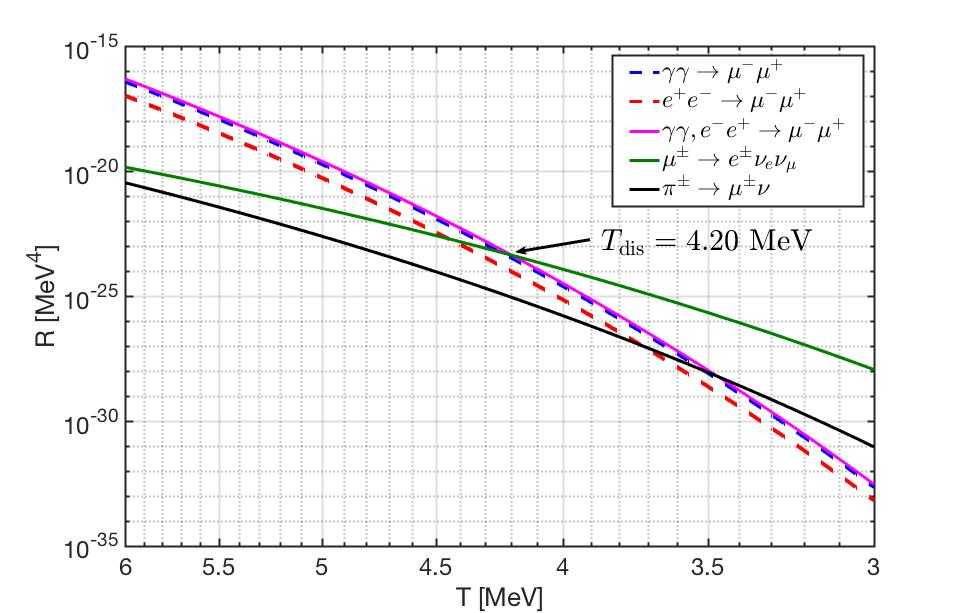
\includegraphics[width=0.9\columnwidth]{./plots/MuonRate_new2.jpg}
\caption{The thermal reaction rate per volume for different reactions as a function of temperature adapted from paper \cite{Rafelski:2021aey}. It shows that dominant reactions for $\mu^\pm$ production are ${\gamma+\gamma\to\mu^++\mu^-}$ and $e^++e^-\to\mu^++\mu^-$, and the total production rate cross the decay rate of $\mu^\pm$ at temperature $T_\mathrm{dis}\approx 4.20$ MeV.}
\label{muon_fig} 
\end{figure}
%~~~~~~~~~~~~~~~~~~~~~~~~~~~~~~~~~~~~~~~~~~~~~~~~~~~~~~~~~~~~~~~`

%~~~~~figure~~~~~~~~~~~~~~~~~~~~~~~~~~~~~~~~~~~~~~~~~~~~~~~~~~~~~~~`
\begin{figure}[t]
%\begin{center}
\centering
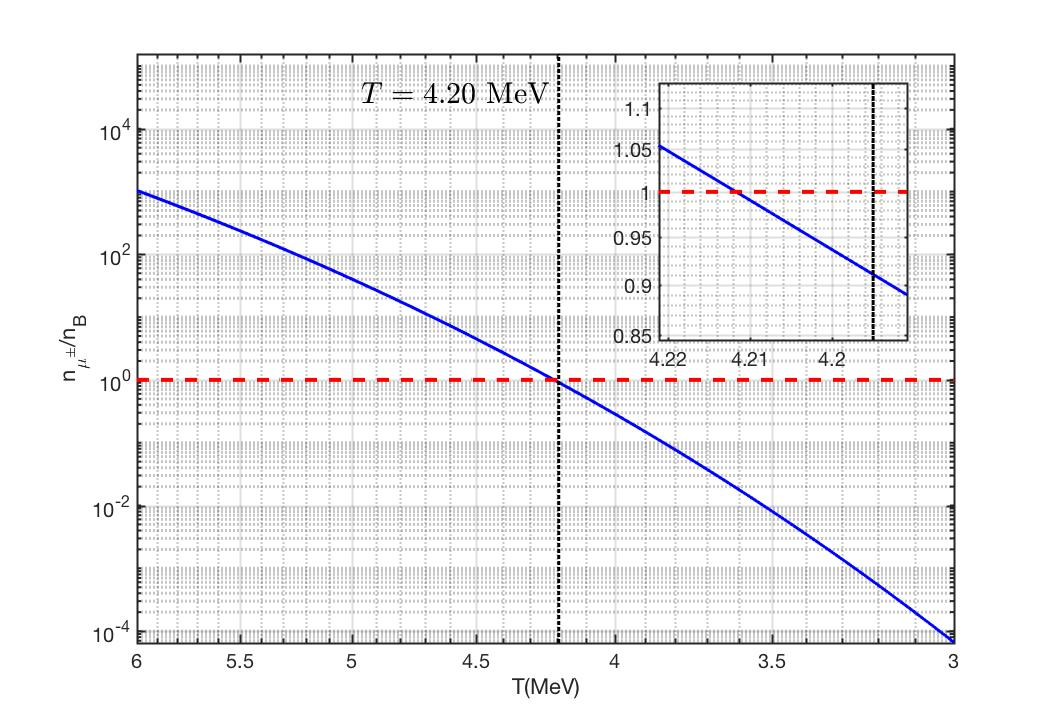
\includegraphics[width=0.9\columnwidth]{./plots/DensityRatio_new2.jpg}
\caption{The density ratio between $\mu^\pm$ and baryons as a function of temperature. The density ratio at muon disappearance temperature is about $n_{\mu^\pm}/n_\mathrm{B}(T_\mathrm{dis})\approx0.911$.}
\label{muonRatio_fig} 
\end{figure}
%~~~~~~~~~~~~~~~~~~~~~~~~~~~~~~~~~~~~~~~~~~~~~~~~~~~~~~~~~~~~~~~`
As the temperature decreases in the expanding Universe, the initially dominant production rates become smaller and cross the decay rates. Muon abundance disappears as soon as any decay rate is faster than the fastest production rate. Considering the slow speed of the Universe's expansion the muon disappearance is sudden, the muon abundance thus disappears as soon as a decay rate crosses the dominant production rate. Specifically, after the Universe cools below the temperature $T_\mathrm{dis} = 4.20$ MeV, the dominant reaction is the muon decay.

In Fig(\ref{muonRatio_fig}) we show the density ratio at $T=T_\mathrm{dis}$ is $n_{\mu^\pm}/n_\mathrm{B}\approx0.91$ \cite{Yang:2021bko} . This means that the muon abundance may still be able to influence baryon evolution because their number density is comparable to the baryon density. This offers a new and tantalizing model-building opportunity for  baryon-antibaryon separation in the primordial Universe, strangelet formation, and perhaps other exotic primordial structure formation mechanisms.

%%%%%%%%%%%%%%%%%%%%%%%%%%%%%%%%%%%%%%%
\subsection{Neutrino Masses and Oscillation} \label{sec:Neutrinos}
\noindent Neutrinos are believed to have a small, but nonzero mass due to the phenomenon of flavor oscillation. This is seen in the flux of neutrinos from the Sun, and also in terrestrial reactor experiments. In the Standard Model neutrinos are produced via weak charged current (mediated by the W boson) as flavor eigenstates. If the neutrino was truly massless, then whatever flavor was produced would be immutable as the propagating state. However, if neutrinos have mass, then they propagate through space as their mass-momentum eigenstates. A flavor eigenstate $\nu^{\alpha}$ can be described as a superposition of mass eigenstates $\nu^{k}$ with coefficients given by the Pontecorvo–Maki–Nakagawa–Sakata (PMNS) mixing matrix which both generally complex and unitary. This is given by
\begin{align}\label{NuFlavors}
	\nu^{\alpha}=\sum_k^nU^\ast_{\alpha k}\nu^{k}, \qquad\alpha=e,\mu,\tau,\qquad k=1,2,3,\dots,n
\end{align}
where $U$ is the PMNS mixing matrix. The PMNS matrix is the lepton equivalent to the CKM mixing matrix which describes the misalignment between the quark flavors and their masses. The parameter $\delta$ is the CP-violating phase which is present when the number of generations is $n\geq3$. In principle, the number of mass eigenstates can exceed three, but is restricted to three generations in most models. By standard convention found in the literature we parameterize the rotation matrix $U$ as
	\begin{alignat}{1}
  	\label{PMNS} U =
		\begin{pmatrix}
			c_{12}c_{13} & s_{12}c_{13} & s_{13}e^{-i\delta}\\
			-s_{12}c_{23} - c_{12}s_{13}s_{23}e^{i\delta} & c_{12}c_{23} - s_{12}s_{13}s_{23}e^{i\delta} & c_{13}s_{23}\\
			s_{12}s_{23} - c_{12}s_{13}c_{23}e^{i\delta}& -c_{12}s_{23} - s_{12}s_{13}c_{23}e^{i\delta} & c_{13}c_{23}
		\end{pmatrix}\,,
	\end{alignat}
where $c_{ij} = \mathrm{cos}(\theta_{ij})$ and $s_{ij} = \mathrm{sin}(\theta_{ij})$. In this convention, the three mixing angles $(\theta_{12}, \theta_{13}, \theta_{23})$, are understood to be the Euler angles for generalized rotations.

Neutrino masses can be written in terms of an effective theory where the mass term contains various couplings between neutrino states determined by some BSM theory. The exact form of such a BSM theory is outside the scope of this work. In modeling the neutrino masses, we have two standard Lagrangian choices. The first is the Dirac mass given by
\begin{alignat}{1}
	\label{DiracMass} \mathcal{L}_{m}^{Dirac} = -\bar{\nu}^{\alpha}_{L}M^{D}_{\alpha\beta}\nu^{\beta}_{R}+\mathrm{h.c.}
\end{alignat}
which requires both left $L$ and right-handed $R$ neutrinos. Under weak $SU(2)_{L}$ symmetry, such right-handed neutrinos would be sterile and otherwise not couple to the Standard Model. In general, the mass matrix $M$ can be complex and contains off diagonal elements which arise from coupling between flavors. The PMNS mixing matrix is then responsible for diagonalizing the mass matrix and reorganizing the neutrinos into a new set of basis states. The corresponding Majorana fermion mass term in the flavor basis is then given by
\begin{alignat}{1}
	\label{Majorana} \mathcal{L}_{m}^{Maj.} = -\frac{1}{2}\bar{\nu}^{\alpha}_{L}M^{M}_{\alpha\beta}(\nu^{\beta}_{L})^{c}+\mathrm{h.c.}\,,
\end{alignat}
where $\nu^{c} = \hat{C}(\bar{\nu})^{T}$ is the charge conjugate of the neutrino field. The operator $\hat{C} = i\gamma^{2}\gamma^{0}$ is the charge conjugation operator. A third option is to consider neutrinos with both Dirac and Majorana mass Lagrangians. If the masses are generated at some high scale, the See-Saw mechanism ensures that the degrees of freedom separate into heavy sterile neutrinos and light nearly massless neutrinos. The See-Saw mechanism then provides an explanation for the smallness of the neutrino masses as has been experimentally observed. Sterile neutrinos of any mass have not yet been observed despite extensive searching. The existence of such neutrinos, if they were ever thermally active in the early cosmos would leave fingerprints on the Cosmic Neutrino Background (CNB) spectrum \cite{Birrell:2014qna}. The presence of an abnormally large anomalous magnetic moment \cite{Morgan:1981zy,Fukugita:1987uy,Vogel:1989iv,Elmfors:1997tt,Giunti:2008ve,Giunti:2014ixa,Canas:2015yoa} for the neutrino would also possibly leave traces in the evolution of the early Universe.

The neutrino eigenmasses are generally considered to be small with values no more than $0.1\eV$. Because of this, neutrinos produced during fusion within the Sun or radioactive fission in terrestrial reactors on Earth propagate relativistically. Evaluating freely propagating plane waves in the relativistic limit yields the vacuum oscillation probability between flavors $\nu_\alpha$ and $\nu_\beta$ written as
\begin{align}\label{NuOscillation}
    P_{\alpha\rightarrow\beta}
    =\left|\sum_{j}U^{\ast}_{\alpha j}U_{\beta j}\exp{\left(-i\frac{\Delta m^2_{kj}}{2E}L\right)}\right|^{2},\qquad\Delta m^2_{kj}\equiv{m^2_k-m^2_j}
\end{align}
where $L$ is the distance traveled by the neutrino between production and detection. The square mass difference $\Delta m^2_{kj}$ has been experimentally measured \cite{ParticleDataGroup:2022pth}. As oscillation only restricts the differences in mass squares, the precise values of the masses cannot be determined from oscillation experiments alone. It is also unknown under what hierarchical scheme the masses are organized as two of the three neutrino eigenmasses are close together in value. If the two lightest neutrinos are close together in mass, this is referred to as normal hierarchy, while if the two heaviest neutrinos are close together we have an inverted hierarchy. It is important to point out that oscillation does not represent any physical interaction or change in the neutrino during propagation. Rather, for a given production energy, the superposition of mass eigenstates each have unique momentum and thus unique group velocities. This mismatch in the wave propagation leads to the oscillatory probability of flavor detection as a function of distance.

In our work on neutrino freezeout \cite{Birrell:2012gg}, we did not consider oscillations during the freezeout period. We expect though that incorporating oscillations into the freezeout calculation would yield a smaller freezeout temperature difference between neutrino flavors as oscillation provides a mechanism in which the heavier flavors remain thermally active despite their direct production becoming shutdown. In work by Mangano et. al. \cite{Mangano:2005cc}, neutrino freezeout including flavour oscillations is shown to be a negligible effect.

%%%%%%%%%%%%%%%%%%%%%%%%%%%%%%%%%%%%%%%
\subsection{Neutrino freezeout in early Universe}\label{sec:Freezeout}
\noindent The relic neutrino background is believed to be a  well-preserved probe of a Universe only a second old. The properties of the neutrino background are influenced by the details of the freeze-out or decoupling process at a temperature $T=\mathcal{O}(1\MeV)$. In general, The freeze-out process, whereby a particle species stops interacting and decouples from the photon background, involves several steps that lead to the final form of the free-streaming momentum distribution. We outline the freezeout properties, including what distinguishes it from the equilibrium distributions as follow\cite{Birrell:2012gg}:
\begin{itemize}
  \item
Chemical freeze-out of a particle species occurs at the temperature, 
$T_{ch}$, when particle number changing processes slow down and the particle abundance can no longer be maintained at an equilibrium level. Prior to the  chemical freeze-out temperature,  number changing processes are significant and keep the particle in chemical (and thermal) equilibrium, implying that the distribution function has the Fermi-Dirac form, obtained by maximizing entropy at fixed energy
\begin{equation}\label{equilibrium}
f_{c}(t,E)=\frac{1}{\exp(E/T)+1}, \text{ for } T(t)> T_{ch}.
\end{equation}

\item
Kinetic freeze-out occurs at the temperature, $T_f$, when momentum exchanging interactions no longer occur rapidly enough to maintain an equilibrium momentum distribution. When $T_f<T(t)<T_{ch}$, the number-changing process  no longer occurs rapidly enough to keep the distribution in chemical equilibrium but there is still sufficient momentum exchange to keep the distribution in thermal equilibrium.  The distribution function is therefore obtained by maximizing entropy, with fixed energy, particle number, and antiparticle number separately,  implying that the distribution function has the form
\begin{equation}\label{kinetic_equilib}
f_k(t,E)=\frac{1}{\Upsilon^{-1}\exp(E/T)+1}, \text{ for }T_f< T(t)< T_{ch}.
\end{equation}
The fugacity
\begin{equation}
\Upsilon(t)\equiv e^{\sigma(t)}
\end{equation}
 controls the occupancy of phase space and is necessary once $T(t)<T_{ch}$ in order to conserve particle number. See \cite{Birrell:2012gg} for a detailed discussion of its significance.
 
\item
For $T(t)<T_f$ there are no longer any significant interactions that couple the particle species of interest and so they begin to free-stream through the Universe, i.e. travel on geodesics without scattering.  The Einstein Vlasov equation can be solved, see \cite{choquet2008general}, to yield the free-streaming momentum distribution
\begin{equation}\label{free_stream_dist}
f(t,E)=\frac{1}{\Upsilon^{-1}e^{\sqrt{p^2/T^2+m^2 /T_f^2}}+ 1}
\end{equation}
where the free-streaming effective temperature
\begin{equation}\label{T_freestream_dist}
T(t)=\frac{T_fa(t_k)}{a(t)}
\end{equation}
is obtained by redshifting the temperature at kinetic freeze-out. The corresponding free-streaming energy density, pressure, and number densities are given by
\begin{align}
\rho&=\frac{d}{2\pi^2}\!\int_0^\infty\!\!\!\frac{\left(m^2+p^2\right)^{1/2}p^2dp }{\Upsilon^{-1}e^{\sqrt{p^2/T^2+m^2/T_f^2}}+ 1},\label{freestream_rho}\\[0.2cm]
P&=\frac{d}{6\pi^2}\!\int_0^\infty\!\!\!\frac{\left(m^2+p^2\right)^{-1/2}p^4dp }{\Upsilon^{-1} e^{\sqrt{p^2/T^2+m^2/T_f^2}}+ 1},\label{freestream_P}\\[0.2cm]
n&=\frac{d}{2\pi^2}\!\int_0^\infty\!\!\!\frac{p^2dp }{\Upsilon^{-1}e^{\sqrt{p^2/T^2+m^2/T_f^2}}+ 1},
\label{num_density}
\end{align}
where $d$ is the degeneracy of the particle species. These differ from the corresponding expressions for an equilibrium distribution in Minkowski space by the replacement $m\rightarrow m T(t)/T_f$  {\em only} in the exponential. 
\end{itemize}
The separation of the freeze-out process into these three regimes is of course only an approximation.  In principle, there is a smooth transition between them.  However, it is a very useful approximation in cosmology.  See \cite{Mangano:2005cc,Birrell:2014gea} for methods capable of resolving these smooth transitions.


%%%%%%%%%%%%%%%%%%%%%%%%%%%%%%%%%%%%%%%
\begin{figure}[ht]
\centerline{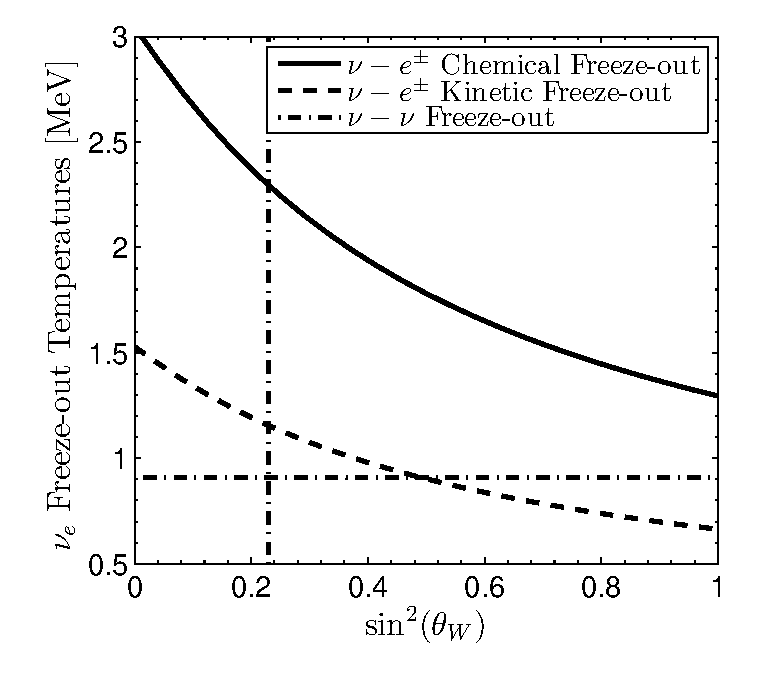
\includegraphics[width=0.47\columnwidth]{./plots/nu_e_freezeout.eps}
\hspace{1mm}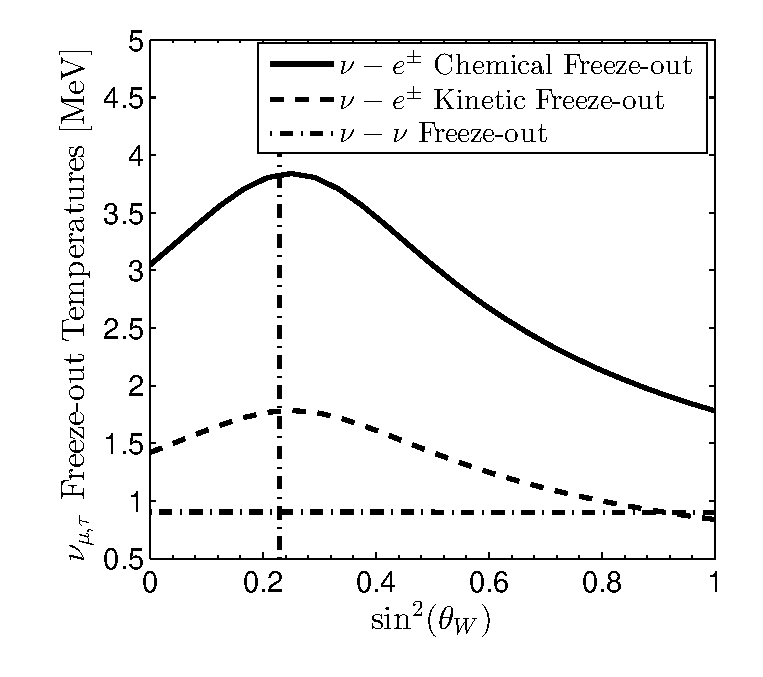
\includegraphics[width=0.47\columnwidth]{./plots/nu_mu_freezeout.eps}}
\centerline{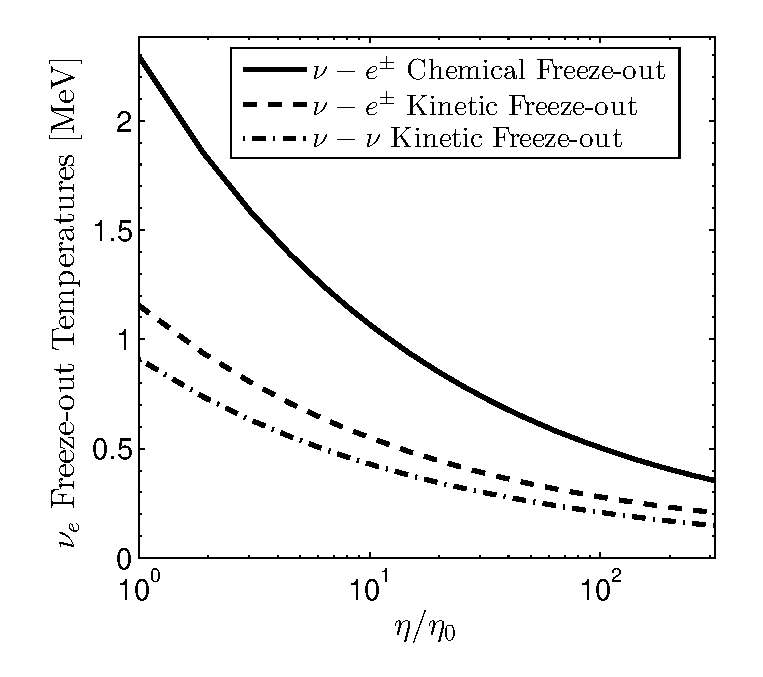
\includegraphics[width=0.47\columnwidth]{./plots/nu_e_freezeout_GF.eps}
\hspace{1mm}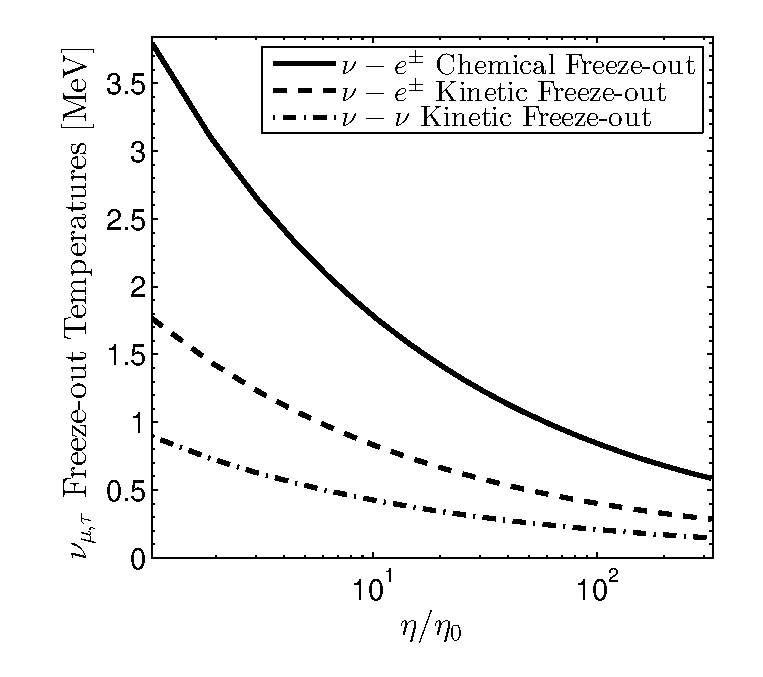
\includegraphics[width=0.47\columnwidth]{./plots/nu_mu_freezeout_GF.eps}}
\caption{Freeze-out temperatures for electron neutrinos (left) and $\mu$, $\tau$ neutrinos (right) for the three types of processes adapted from paper \cite{Birrell:2014uka}. Top panels as functions of $\sin^2\theta_W$ for $\eta=\eta_0$, the vertical line is $\sin^2\theta_W=0.23$; bottom panels  as a function  of relative change in interaction strength $\eta/\eta_0$ obtained  for $\sin^2\theta_W=0.23$. Figure reprinted from our earlier work \cite{Birrell:2014uka}.}
\label{fig:freezeoutT}%\label{fig:Weinberg_freezeout}\label{fig:GF_freezeout}
 \end{figure}
%%%%%%%%%%%%%%%%%%%%%%%%%%%%%%%%%%%%%%%

 To estimate the freezeout temperature we need to solve the Boltzmann equation with different types of collision terms. In paper \cite{Birrell:2014uka} we detail a new method for analytically simplifying the collision integrals and show that the neutrino freezeout temperature which is in turn controlled by the standard model (SM) of particle physics  parameters. The freezeout temperature depends only on the magnitude of the Weinberg angle in the form $\sin^2\theta_W$ , and a dimensionless relative interaction strength parameter $\eta$,
\begin{align}
\eta\equiv M_p m_e^3 G_F^2, \qquad M_p^2\equiv \frac{1}{8\pi G_N}, \end{align}
a combination of  the electron mass $m_e$, Newton constant $G_N$, and the Fermi constant $G_F$. The dimensionless interaction strength parameter $\eta$ with the vacuum present-day value is given by
\begin{align}
\eta_0\equiv \left.M_p m_e^3 G_F^2\right|_0  = 0.04421 .
\end{align}
The magnitude of  $\sin^2\theta_W$ is not fixed within the SM and  could be subject to variation as a function of time or temperature. In Fig.(\rf{fig:freezeoutT}) we show the dependence of neutrino freezeout temperatures for $\nu_e$ and $\nu_{\mu,\tau}$ on SM model parameters  $\sin^2\theta_W$ and $\eta$ in detail. The impact of SM parameter values on neutrino freeze-out and the discussion of the implications and connections of this work to other areas of physics, namely Big Bang Nucleosynthesis and dark radiation can be found in detail in \cite{Dreiner:2011fp,Boehm:2012gr,Blennow:2012de,Birrell:2014uka}.

 After neutrinos freezeout, the neutrino comoving entropy is independently conserved. However, the presence of electron-positron rich plasma until $T=20\keV$ provides the reaction $\gamma\gamma\to e^-e^+\to\nu\bar{\nu}$ to occur even after neutrinos decouple from the cosmic plasma. This suggests the small amount of $e^\pm$ entropy can still transfer to neutrinos until temperature $T=20\keV$ and can modify free streaming distribution and the effective number of neutrinos.
%%%%%%%%%%%%%%%%%%%%%%%%%%%%%%%%%%%%%%%%%%%%%%%%%%%%%%%%%%%%%%%%%%%
\subsection{Effective Number of Neutrinos}\label{sec:EffectiveNeutrino}
\noindent The population of each flavor of neutrino is not a fixed quantity throughout the evolution of the Universe. In the earlier hot Universe, the population of neutrinos is controlled thermally and to maximize entropy, each flavor is equally filled. As the expansion factor $a(t)$ is radiation dominated for much of this period (see \rf{CosmicFraction}), the CMB is ultimately sensitive to the total energy density within the neutrino sector (which is sometimes referred to as the \lq\lq dark radiation\rq\rq\ contribution). This is described by the effective number of neutrinos $N_{\nu}^{\mathrm{eff}}$ and captures the number of relativistic degrees of freedom.
\begin{align}\label{Neff}
N_\nu^{\mathrm{eff}}\equiv\frac{\rho^{\mathrm{tot}}_\nu}{\frac{7\pi^2}{120}\left(\frac{4}{11}\right)^{4/3}T_\gamma^4}\;,
\end{align}
where $\rho_\nu^{\mathrm{tot}}$ is the total energy density in neutrinos and $T_\gamma$ is the photon temperature. $N_\nu^{\mathrm{eff}}$ is defined such that three neutrino flavors with zero participation of neutrinos in reheating during $e^+e^-$ annihilation results in $N_\nu^{\mathrm{eff}}=3$. The factor of $\left(4/11\right)^{1/3}$ relates the photon temperature to the (effective) temperature of the free-streaming neutrinos \cite{Coleman:2003hs} after $e^\pm$ annihilation, under the assumption of zero neutrino reheating.

Naively speaking, this number should take on the value near $N_{\nu}^{\mathrm{eff}}\approx3$, which fits within the Planck result of $N_{\nu, exp}^{\mathrm{eff}}=2.99\pm0.17$ \cite{Planck:2018vyg}. This number in the $\Lambda$-CDM model is expected to deviate slightly to a value of $N_{\nu, \Lambda CDM}^{\mathrm{eff}}=3.046$ due to an overpopulation of the $\nu_{e}$ electron-neutrino flavor during BBN in the production of the light elements. We also note that this number is subject to change from a more accurate assessment of lithium and tritium production, neutrino masses, as well as neutrino production from the positron disappearance event shortly after BBN. Low energy bound-state electron-positron (positronium) decay into neutrinos is suppressed as $m_{\nu}^{2}/m_{e}^{2}$ \cite{Govaerts:1996dt,Adkins:2022omi} but may be enhanced by neutrino anomalous magnetic moment. This situation however does not describe the disappearance of the positrons which was a \lq\lq hot\rq\rq\ scattering process where the $e^{+}e^{-}\rightarrow\gamma\gamma$ amplitude outpaced the reverse $\gamma\gamma\rightarrow e^{+}e^{-}$ production process as the Universe cooled. With that in mind, the neutrino anomalous moment contribution to neutrino degrees of freedom in $e^{\pm}$ epoch should be explored. The neutrino degrees of freedom are also sensitive to the presence of sterile neutrinos \cite{Joudaki:2012uk,Birrell:2014uka} which is a common feature of many BSM models. We note that the Planck result is not well constrained and thus an important place to look for deviations away from standard model results.

The currently accepted theoretical value is $N_\mathrm{eff}=3.046$, after including the slight effect of neutrino reheating. The favored value of $N_\mathrm{eff}$ can be found by fitting to CMB data. In 2013 the Planck collaboration found $N_\mathrm{eff}=3.36\pm0.34$ (CMB only) and $N_\mathrm{eff}=3.62\pm0.25$ (CMB and H0). As $N_\mathrm{eff}$ is only a measure of the relativistic energy density leading up to photon decoupling, a natural alternative mechanism for obtaining $N_\mathrm{eff}>3$ is the introduction of additional, presently not
discovered, weakly interacting massless particles \cite{Anchordoqui:2011nh,Abazajian:2012ys,Anchordoqui:2012qu,Steigman:2013yua,Giusarma:2014zza}
 The explanations of the tension in $N_\mathrm{eff}$ has already inspired various theories, including the consideration of:
\begin{itemize}
\item Neutrino freezeout condition and $N_\nu^{\mathrm{eff}}$:\\
A precise study of the neutrino decoupling condition can provide precise predictions of $N_\nu^{\mathrm{eff}}$. A lot of studies focus on improving the calculation of decoupling, including:
1.)model in which the temperature of neutrino decoupling was a variable standard model of particle physics parameters \cite{Birrell:2014uka,Birrell:2014ona}, 2.) The entropy transfer from electron-positron annihilation and finite temperature correction at neutrino decoupling \cite{Dicus:1982bz,Heckler:1994tv,Fornengo:1997wa}, 3.) Neutrino decoupling with flavor oscillations \cite{Mangano:2005cc,Mangano:2001iu}, provide precise predictions. 4.) Nonstandard neutrino interactions have been investigated, including neutrino electromagnetic \cite{Mangano:2006ar,Morgan:1981zy,Elmfors:1997tt,Fukugita:1987uy,Giunti:2008ve,Vogel:1989iv} and nonstandard neutrino electron coupling \cite{Mangano:2006ar}
\item QGP as the possible source contribute to $N_\nu^{\mathrm{eff}}$:\\
The natural concordance of the reported CMB range of $N_\nu^{\mathrm{eff}}$ with the range of QGP hadronization temperatures, motivates the exploration of a connection between $N_\nu^{\mathrm{eff}}$ and the decoupling of sterile particles at and below the QGP phase transition\cite{Birrell:2014cja}. It shows that $N_\nu^{\mathrm{eff}}>3.05$ can be associated with the appearance of several light particles at QGP hadronization in the early Universe that either is weakly interacting in the entire space or is allowed to interact only inside the deconfined domain, in which case their coupling would be strong. Such particles could leave a clear experimental signature in relativistic heavy-ion experiments that produce the deconfined QGP phase.

\item Connection between lepton asymmetry $L$ and $N_\nu^{\mathrm{eff}}$:\\
In the current standard cosmological model, an asymmetry between leptons and anti-leptons $L\equiv  [N_\mathrm{L}-N_{\overline{\mathrm{L}}}] /N_\gamma $  (normalized with the photon number) is in general assumed to be small (nano-scale) so that the net normalized lepton number equals the net baryon number $L=B$ where $B=[N_\mathrm{B}-N_{\overline{\mathrm{B}}}]/N_\gamma $. Barenboim, Kinney, and Park~\cite{Barenboim:2016shh,Barenboim:2017dfq}  note that the lepton asymmetry of the Universe is one of the most weakly constrained parameters and propose leptogenesis scenarios able to accommodate a large lepton number asymmetry surviving up to this date. The work \cite{Yang:2018oqg}  extend their qualitative discussion of these constraints by quantifying the impact of large lepton asymmetry on Universe expansion and shows that there is another \lq natural\rq\ choice  $L\simeq 1$, making the  net lepton number and net photon number in the Universe similar. 

\end{itemize}
In summary, the effective number of neutrinos $N_\nu^{\mathrm{eff}}$ is a characterization of the relativistic energy content
in the early Universe and independent of its source. Thus, even given a the noninteger number of neutrino degrees of freedom $N_\nu^{\mathrm{eff}}$ reported experimentally, there would still remain ambiguity in regard the origin of the effect.
%%%%%%%%%%%%%%%%%%%%%%%%%%%%%%%%%%%%%%%
\section{Electron-Positron Epoch}\label{sec:ElectronPositron}
\noindent The electron-positron epoch of the early Universe was home to several significant events which have greatly shaped our contemporary Universe including neutrino decoupling, Big Bang Nucleosynthesis (BBN), the annihilation of most electrons and positrons partially re-ionizing the Universe, as well as setting the stage for the eventual recombination period which would generate the cosmic microwave background (CMB). Therefore, correctly describing the dynamics of this $e^{\pm}$ plasma is of interest when considering modern cosmic mysteries such as the origin of extra-galactic magnetic fields (EGMF) \cite{Anchordoqui:2001bs,Neronov:2010gir}. While most approaches tackle magnetized plasmas from the perspective of classical or semi-classical magneto-hydrodynamics (MHD) \cite{berezhiani1992influence,berezhiani1995large,Schlickeiser:2018hzq}, our perspective is to demonstrate that fundamental quantum statistical analysis can lead to further insights on the behavior of magnetized plasmas.

The properties of the electron-positron $e^{\pm}$ plasma in the early Universe has not received appropriate attention in an era of precision BBN studies~\cite{Pitrou:2018cgg}. The presence of $e^{\pm}$ pairs before and during BBN has been acknowledged by Wang, Bertulani and Balantekin~\cite{Wang:2010px} over a decade ago. This however was before necessary tools were developed to explore the connection between electron and neutrino plasmas~\cite{Mangano:2005cc,Birrell:2012gg,Birrell:2014uka}. 

In \rf{Density_fig} we show that the dense $e^{\pm}$ plasma in the early Universe under the hypothesis charge neutrality and entropy conservation as a function of temperature $2\,\mathrm{MeV}>T>10\,\mathrm{keV}$ \cite{Chris:2023abc}. The plasma is electron-positron rich, i.e, $n_{\pm}\gg n_B$ in the early Universe until leptonic annihilation at $T_{\mathrm{split}} = 20.36\ \mathrm{keV}$. For $T<T_{\mathrm{split}}$ the positron density $n_{e^+}$ decreases dramatically because of annihilation and the residual electron density becomes equal to the proton density in accordance with charge neutrality in the Universe as a whole.
\begin{figure}[htbp]
  \centering  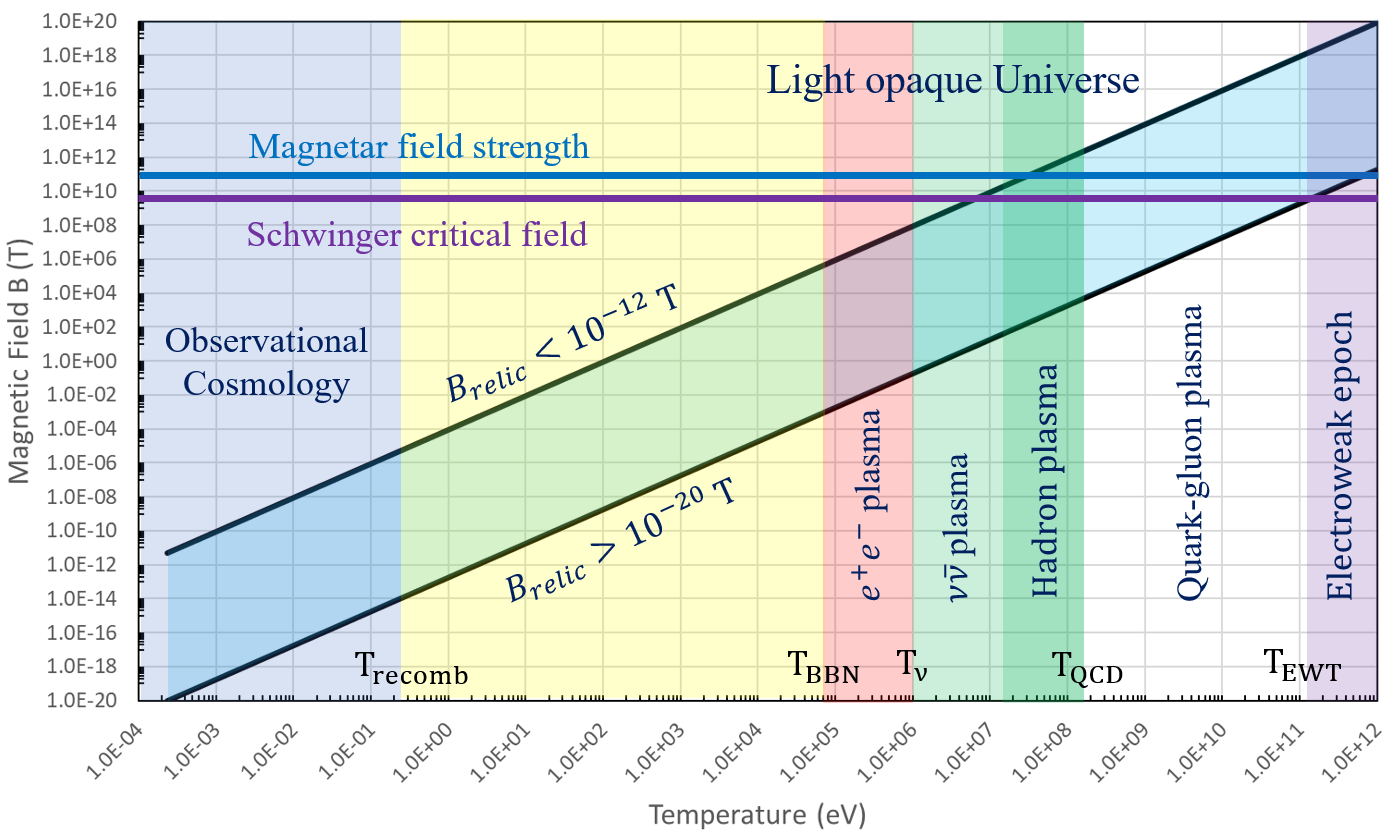
\includegraphics[trim=110 50 120 40,clip,width=\textwidth]{./plots/relic_plot.PDF}
  \caption{Qualitative value of the primordial magnetic field over the evolutionary lifespan of the Universe. The upper and lower black lines represent extrapolation of the EGMF bounds into the past. The major phases of the universe are indicated with shaded regions. The values of the Schwinger critical field (purple line) and the upper bound of surface magnetar field strength (blue line) are included for scale.\label{relic_plot}}
\end{figure}

We can now connect back to the consideration of cosmic magnetic fields as they might have risen in the environment of early Universe plasmas noting that such primordial magnetic fields would be lensed through each of the various plasmas that existed when the Universe was far hotter and denser. As magnetic flux is conserved over co-moving surfaces, we see in \rf{relic_plot} that the primordial relic field is expected to dilute as $B\propto1/a(t)^{2}$. This means the contemporary small bounded values of $5\times10^{-12}\ \mathrm{T}>B_{relic}>10^{-20}\ \mathrm{T}$ (coherent over $\mathcal{O}(1\ \mathrm{Mpc})$ distances) may have once represented large magnetic fields in the early Universe. This is relic magnetic field would then be generated by the last phase of significant magnetization in the early Universe. This figure is meant to be illustrative and it is unlikely the magnetization of the Universe would proceed unhindered and unaltered into the ultra-dense plasma phases of the early Universe. Of particular interest to us is the electron-positron plasma which existed in the early Universe especially at temperatures $T>35\ \mathrm{keV}$ which was the last matter(antimatter) plasma in the Universe where the energy its density exceeded that of the proton/neutron baryon energy density. This dense plasma environment is where BBN occurred and where similar plasmas can still be found within exotic stars such as magnetar \cite{Broderick:2000pe}s. The contemporary relic magnetic fields may then be an artifact of this final time of Universe-scale magnetization in a manner similar to how the CMB is a relic of the time of charge recombination.

The Universe is filled with magnetic fields \cite{Kronberg:1993vk} at various scales and strengths both within galaxies and in deep extra-galactic space far and away from matter sources. Extra-galactic magnetic fields are not well constrained today, but are required by observation to be non-zero \cite{Anchordoqui:2001bs,Widrow:2002ud} with a magnitude between $10^{-12}\ \mathrm{T}>B_{EGMF}>10^{-20}\ \mathrm{T}$ over Mpc coherent length scales. The upper bound is constrained from the characteristics of the CMB while the lower bound is constrained by non-observation of ultra-energetic photons from blazars \cite{Neronov:2010gir}. There are generally considered two possible origins \cite{Widrow:2011hs,Vazza:2021vwy} for extra-galactic magnetic fields: (a) matter-induced dynamo processes involving Amperian currents and (b) primordial (or relic) seed magnetic fields whose origins may go as far back as the Big Bang itself. It is currently unknown which origin accounts for extra-galactic magnetic fields today or if it some combination of the two models. Even if magnetic fields in the Universe today are primarily driven via amplification through Amperian matter currents, such models still require primordial seed fields at some point to act as catalyst.
\subsection{Electron-Positron Density Compared to Baryons}\label{sec:ElectronPositronDensity}
\noindent During the late stages of the $e^{\pm}$ epoch where BBN occurred, the matter content of the Universe was still mostly dominated by the light charged leptons by many orders of magnitude even though the Hubble parameter was still mostly governed by the radiation behavior of the neutrinos and photons. The temperatures during this epoch were also cool enough that the electrons and positrons could be described non-relativistically to fairly good approximation while also still being as energy dense as the Solar core making it a relatively unique plasma environment not present elsewhere in cosmology. Considering the energy density between non-relativistic $e^{\pm}$ and baryon, it can be written as
\begin{align}\label{Eq_ratio}
\chi\equiv\frac{\rho_e+\rho_{\bar e}}{\rho_p+\rho_n}=\frac{m_e(n_e+n_{\bar e})}{m_pn_p+m_n n_n}=\frac{m_e(n_e+n_{\bar e})}{n_B(m_pX_p+m_nX_n)}=\left(\frac{n_e+n_{\bar e}}{n_B}\right)\,\left(\frac{m_e}{m_pX_p+{m_n X_\alpha}/2}\right)
\end{align}
where we consider all neutrons end up bound in to the $^4H_e$ after BBN  and from particle data group $X_p=n_p/n_B$ and $X_\alpha=n_\alpha/n_B$ and are given by
\begin{align}
X_p=0.878,\qquad X_\alpha=0.245
\end{align}
and masses are given by
\begin{align}
m_e=0.511\,\mathrm{MeV}, \qquad m_p=938.272\,\mathrm{MeV},\qquad m_n=939.565\,\mathrm{MeV}
\end{align}
In \rf{ratio_fig} we plot the energy density ratio \req{Eq_ratio} as a function of temperature $10\,\mathrm{keV}< T<200\,\mathrm{keV}$. It shows that the energy density of electron and positron is dominated until $T=30.2$ keV, i.e.,  we have $\rho_{e}\gg\rho_B$.  Until around $T\approx50\keV$, the $e^{\pm}$ density remained higher than that of the solar core, though notably at a much higher temperature than the Sun's core at $T_{\odot}=1.36\keV$ \cite{Castellani:1996cm}. After $T=30.2$ keV, we have $\rho_{e}\ll\rho_B$ and ratio becomes constant when is around $T=20$keV because of the positron annihilation and charge neutrality.

%%%%%%%%%%%%%%%%%%%%%%%%%%%%%%%%%%%%%%%
\begin{figure}[ht]
%\begin{center}
\centering
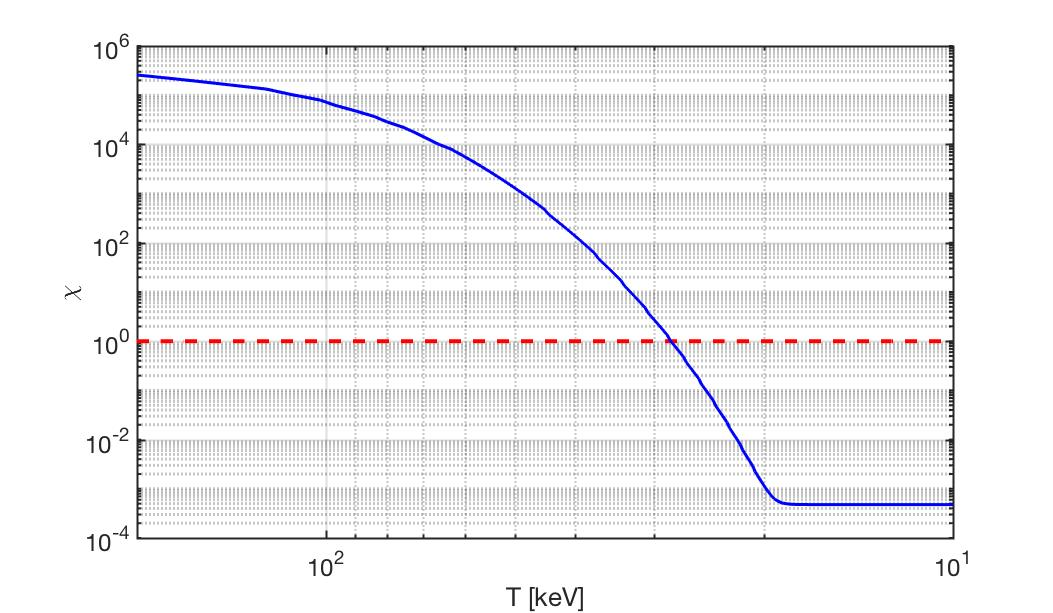
\includegraphics[width=\textwidth]{./plots/EnergyDensityRatio002.jpg}
\caption{The energy density ratio $\chi$ (solid blue line) between $e^{\pm}$ and baryons as a function of temperature from $10\,\mathrm{keV}< T<200\,\mathrm{keV}$. The dashed red line represents the point where the baryon density exceeds that of the electron-positron pairs.}
\label{ratio_fig} 
\end{figure}
%%%%%%%%%%%%%%%%%%%%%%%%%%%%%%%%%%%%%%%

\subsection{Energy Eigenvalues}\label{sec:energy}
\noindent As a starting point, we consider the energy eigenvalues of charged fermions within a homogeneous magnetic field. Here, we have several choices: We could assume the typical Dirac energy eigenvalues with gyro-magnetic g-factor set to $g=2$. But as electrons, positrons and most plasma species have anomalous magnetic moments (AMM), we require a more complete model. Another option would be to modify the Dirac equation with a Pauli term, often called the Dirac-Pauli (DP) approach, via
\begin{align}
  \label{Pauli} \hat{H}_{\mathrm{AMM}} = -a\frac{e}{2m_{e}}\frac{\sigma_{\mu\nu}F^{\mu\nu}}{2}\,,
\end{align}
where $\sigma_{\mu\nu}$ is the spin tensor proportional to the commutator of the gamma matrices and $F^{\mu\nu}$ is the EM field tensor. For the duration of this work, we will remain in natural units $(\hbar=c=k_{B}=1)$ unless explicitly stated otherwise. The AMM is defined via g-factor as
\begin{align}
  \label{AMM} \frac{g}{2}=1+a\,.
\end{align}
This approach, while straightforward, would complicate the energies making analytic understanding and clarity difficult without a clear benefit. Modifying the Dirac equation with \req{Pauli} yields the following eigen-energies
\begin{align}
  \label{DPEnergy} E_{n}^{s}\vert_{DP}=\sqrt{\left(\sqrt{m_{e}^{2}+2eB\left(n+\frac{1}{2}-s\right)}-\frac{eB}{2m}(g-2)s\right)^{2}+p_{z}^{2}}
\end{align}
This model for the electron-positron plasma of the early Universe has been used in work such as Strickland et. al. \cite{Strickland:2012vu}. Our work here is then in part a companion peice which compares and contrasts the DP model of fermions to our preferred model for the AMM via the Klein-Gordon-Pauli (KGP) equation given by
\begin{alignat}{1}
  \label{KGP} \left(\left(i\partial_{\mu}-eA_{\mu}\right)^{2}-m_{e}^{2}-e\frac{g}{2}\frac{\sigma_{\mu\nu}F^{\mu\mu}}{2}\right)\Psi=0\,.
\end{alignat}
We wish to emphasize, that each of the three above models (Dirac, DP, KGP) are distinct and have differing physical consequences and are not interchangeable which we explored in the context of hydrogen-like atoms in \cite{Steinmetz:2018ryf}. Recent work done in \cite{rafelski2023study} discuss the benefits of KGP over other approaches for $g\neq2$ from a quantum field theory perspective. Exploring the statistical behavior of KGP in a cosmological context can lead to new insights in magnetization which may be distinguished from pure $g=2$ behavior of the Dirac equation or the \emph{ad hoc} modification imposed by the Pauli term in DP. One major improvement of the KGP approach over the more standard DP approach is that the energies take eigenvalues which are mathematically similar to the Dirac energies. Considering the $e^\pm$ plasma in a uniform magnetic field $B$ pointing along the $z$-axis, the energy of $e^\pm$ fermions can be written as
\begin{align}
  \label{KGPEnergy} E_{n}^{s}&=\sqrt{p^2_z+\tilde{m}^2+2eBn},\qquad\tilde{m}^2=m^2_e+eB\left(1-gs\right),\qquad s=\pm\frac{1}{2},\qquad n=0,1,2,3,\dots
\end{align}
where $n$ is the principle quantum number for the Landau levels and $s$ is the spin quantum number. Here we introduce a notion of effective mass $\tilde{m}$ which inherits the spin-specific part of the energy adding them to the mass. This convention is also generalizable to further non-minimal electromagnetic models with more exotic energy contributions such that we write a general replacement as
\begin{align}
  \label{MagMass} m_{e}^{2}\rightarrow\tilde{m}^2(B)\,.
\end{align}
This definition also pulls out the ground state Landau energy separating it from the remainder of the Landau tower of states. One restriction is that the effective mass must remain positive definite in our analysis thus we require
\begin{align}
  \label{MassLimit} \tilde{m}^2(B)=m^2_e+eB\left(1-gs\right)>0\,.
\end{align}
This condition fails under ultra-strong magnetic fields of order
\begin{align}
  \label{MagMassFail} B_{\mathrm{crit}}=\frac{m_{e}^{2}}{ea}=\frac{\mathcal{B}_{S}}{a}\approx3.8\times10^{12}\ \mathrm{T}\,,
\end{align}
where $\mathcal{B}_{S}$ is the Schwinger critical field strength. For electrons, this field strength is well above the window of magnetic field strengths of interest during the late $e^{\pm}$ epoch.

%%%%%%%%%%%%%%%%%%%%%%%%%%%%%%%%%%%%%%%
\subsection{Landau eigen-energies in cosmology}\label{sec:Landau}
\noindent There is another natural scale for the magnetic field besides \req{MagMassFail} when considering the consequences of FLRW expansion on the $e^{\pm}$ fluid. As the Universe expands, different terms in the energies and thus partition function evolve as a function of the scale factor $a(t)$ which arises in the FLRW metric. We can consider the expansion to be an adiabatic process which results in a smooth shifting of the relevant dynamical quantities. From the conservation of magnetic flux through a co-moving surface, the magnetic field under expansion starting at some initial time $t_{0}$ is given by
\begin{alignat}{1}
    \label{BScale} B(t) = B(t_{0})\frac{a(t_{0})^{2}}{a(t)^{2}}\,.
\end{alignat}
As the Universe expands, the temperature also cools as the cosmological redshift reduces the momenta of particles in the Universe lowering their contribution to the energy content of the Universe. This cosmological redshift is written as
\begin{alignat}{1}
  \label{Redshift} p_{i}(t) = p_{i}(t_{0})\frac{a(t_{0})}{a(t)}\,,\qquad T(t) = T(t_{0})\frac{a(t_{0})}{a(t)}\,.
\end{alignat}
The momenta scale with the same factor as temperature as it is the origin of cosmological redshift. The energy of massive free particles in the Universe scales differently based on their momentum (and thus temperature). When hot and relativistic, particle energy scales with inverse scale factors like radiation. However as particles transition to non-relativistic momenta, their energies scale with the inverse square of the scale factor like magnetic flux.
\begin{alignat}{1}
    \label{EScale} E(t) = E(t_{0})\frac{a(t_{0})}{a(t)}\xrightarrow{\mathrm{NR}}\  E(t_{0})\frac{a(t_{0})^{2}}{a(t)^{2}}\,.
\end{alignat}
This occurs because of the functional dependence of energy on momentum in the relativistic versus non-relativistic cases. The argument in the Boltzmann statistical factor is given by
\begin{alignat}{1}
    \label{Boltz} X_{n}^{s}\equiv\frac{E_{n}^{s}}{T}\,.
\end{alignat}
We can explore this relationship for the magnetized system explicitly by writing out \req{Boltz} using the KGP eigen-energies as
\begin{alignat}{1}
    \label{XExplicit} X_{n}^{s} = \sqrt{\frac{m_{e}^{2}}{T^{2}}+\frac{p_{z}^{2}}{T^{2}}+\frac{2eB}{T^{2}}\left(n+\frac{1}{2}-\frac{gs}{2}\right)}\,,
\end{alignat}
where we now introduce the expansion scale factor via \req{BScale} - \req{Redshift}. The Boltzmann factor can then be written as
\begin{alignat}{1}
    \label{XScale} X_{n}^{s}[a(t)] = \sqrt{\frac{m_{e}^{2}}{T^{2}(t_{0})}\frac{a(t)^{2}}{a(t_{0})^{2}}+\frac{p_{z}^{2}(t_{0})}{T^{2}(t_{0})}+\frac{2eB(t_{0})}{T^{2}(t_{0})}\left(n+\frac{1}{2}-\frac{gs}{2}\right)}\,.
\end{alignat}
This reveals that only the mass contribution is dynamic over cosmological time. For any given eigen-state, the mass term increases driving the state into the non-relativistic limit while the momenta and magnetic contributions are frozen by initial conditions.
%We note here one important difference between KGP and DP eigen-energies in the context of cosmology: The anomalous magnetic moment portion of the DP statistics is suppressed by $1/a(t)$ over cosmological time while the AMM contribution is preserved in the KGP model. That the Universe's expansion makes a distinction between $g=2$ magnetic moment and AMM for DP fermions appears as a rather artificial and nonphysical trait. While the suppression of AMM may often be small for particles such as electrons, this suppression is non-trivial for particles with large AMM values such as the proton. That cosmological redshift would push DP protons to be described by $g=2$ eign-energies in the non-relativistic limit counts as a malaise for the model and further strengthens our thinking that the KGP model is more appropriate for cosmological studies.
Following reasoning outlined in \cite{rafelski2023study} and \cite{Steinmetz:2018ryf} we will proceed without analysis using the eigen-energies provided by the KGP equation in favor over modeling the anomalous magnetic moment as a Pauli term added to the Dirac equation (referred to at the Dirac-Pauli equation). Motivated by \req{XScale}, we can introduce a dimensionless cosmic magnetic scale which is frozen in the homogeneous case as
\begin{alignat}{1}
    \label{Bo} b_{0}\equiv\frac{eB}{T^{2}}=\frac{eB\hbar c^{2}}{(k_{B}T)^{2}}\ \mathrm{(S.I)}\,,
\end{alignat}
where we've included the expression explicitly in full SI units. We can estimate the value of $b_{0}$ from the bounds of the extra-galactic magnetic field strength and the temperature of the Universe today.  If the origin of deep space extra-galactic magnetic fields are relic fields from the early Universe, which today are expected to exist between $5\times10^{-12}\ \mathrm{T}>B_{relic}>10^{-20}\ \mathrm{T}$, then at temperature $T=2.7\ \mathrm{K}$, the value of the cosmic magnetic scale is between
\begin{alignat}{1}
    \label{BoScale} 5.5\times10^{-5}>b_{0}>1.1\times10^{-11}\,.
\end{alignat}
This should remain constant in the Universe at-large up to the last epoch the Universe was sufficiently magnetized to disturb this value. As the electron-proton plasma which generated the CMB was relatively dilute over its duration, it was unlikely sufficiently magnetized to significantly alter this value over extra-galactic scales. Rather, the best candidate plasma to have been sufficiently magnetized and dense to have set the relic field magnetic scale would have been the electron-positron plasma which existed during the duration of Big Bang Nucleosynthesis (BBN) and beforehand.

Higher order non-minimal magnetic contributions which can be introduced via \req{MagMass} to the eigen-energies like $\approx\mu_{B}^{2}B^{2}/T^{2}$ are even more suppressed over cosmological time which drives the system into minimal electromagnetic coupling with the exception of the anomalous magnetic moment in the KGP eigenenergies. It is interesting to note that cosmological expansion serves to \lq\lq smooth out\rq\rq\ the characteristics of more complex BSM electrodynamics erasing them from a statistical perspective in favor of the minimal or minimal-like dynamics. As $b_0$ is a constant of expansion, assuming the electron-proton plasma between the CMB and electron-positron annihilation did not greatly disturbed it, we can calculate the remnant values at the temperature $T=50\ \mathrm{keV}$ (which takes place in the middle of BBN) with the expression
\begin{align}
  \label{BBNFields} B(T)=\frac{b_{0}}{e}T^{2}\,,
\end{align}
yielding a range of field strengths
\begin{align}
  \label{BBNRange} 2.3\times10^{5}\ \mathrm{T}>B(T=50\ \mathrm{keV})>4.6\times10^{-4}\ \mathrm{T}\,,
\end{align}
during which the electron-positron plasma in the Universe had a number density comparable to that of the Solar core with $n_{e}=4.49\times10^{24}\ \mathrm{cm}^{-3}$ at $r=0.01R_{\odot}$ \cite{Bahcall:2000nu}. We note that while the density of leptons is comparable to that of the solar core during this period, the temperature is not. The $e^{\pm}$ plasma during BBN was far hotter than the solar core's comparatively cool temperature of $T_{\odot}=1.37\keV$ \cite{Castellani:1996cm}.

%%%%%%%%%%%%%%%%%%%%%%%%%%%%%%%%%%%%%%%
\subsection{Electron-positron statistical physics}\label{sec:Partition}
\noindent We now turn our attention now to the statistical behavior of the $e^{\pm}$ system. We can utilize the general fermion partition function given by \cite{Elze:1980er}
\begin{align}
  \label{PartFunc} \ln\mathcal{Z}=\sum_{\alpha}\ln\left(1+e^{-\beta(E-\eta)}\right)\,,
\end{align}
where $\beta=1/T$, $\alpha$ is the set of all quantum numbers in the system, and $\eta$ is the generalized chemical potential. The magnetized $e^{\pm}$ system should be considered a system of four quantum species: Particles and anti-particles, and spin aligned and anti-aligned. Taken together we consider a system where all electrons and positrons are spin aligned or anti-aligned with the magnetic field $B$ and the partition function of the system is written as
\begin{align}
  \label{PartFuncB}\ln\mathcal{Z}_{tot}=\frac{2eBV}{(2\pi)^2}\sum_{\sigma}^{\pm1}\sum_{s}^{\pm1/2}\sum_{n=0}^\infty\int^\infty_{0}dp_z\left[\ln\left(1+\Upsilon_{\sigma}^{s}(x)e^{-\beta E_{n}^{s}}\right)\right]\,,\\
  \label{Fugacity}\Upsilon_{\sigma}^{s}(x)=\gamma(x)\lambda_{\sigma}^{s}\,,\qquad\lambda_{\sigma}^{s}=e^{\sigma\eta_{e}+s\eta_{s}}\,,
\end{align}
where $\eta_{e}$ is the electron chemical potential and $\eta_s$ is the spin chemical potential for the generalized fugacity $\lambda_{\sigma}^{s}$. The parameter $\gamma(x)$ is a spatial field which controls the distribution inhomogeneity of the Fermi gas. Inhomogeneities can arise from the influence of other forces on the gas such as gravitational forces. Deviations of $\gamma\neq1$ represent configurations of reduced entropy (maximum entropy yields the normal Fermi distribution itself with $\gamma=1$) without pulling the system off a thermal temperature. This situation is similar to that of the quarks during QGP, but instead here the deviation is spatial rather than in time. This is precisely the kind of behavior that may arise in the $e^{\pm}$ epoch as the dominant photon thermal bath keeps the Fermi gas in thermal equilibrium while spatial inequilibria could spontaneously develop. For the remainder of this work, we will retain $\gamma(x)=1$. The energy $E_{n}^\pm$ can be written as
\begin{align}
E_{n}^\pm&=\sqrt{p^2_z+\tilde m^2_\pm+2eBn},\qquad\tilde{m}^2_\pm=m^2_e+eB\left(1\mp\frac{g}{2}\right)\,,
\end{align}
where the $\pm$ script refers to spin aligned and anti-aligned eigenvalues. As the temperature domain we're interested is in the $T=50\ \mathrm{keV}$ range, we can take a semi-relativistic approach of the electron-positron plasma by considering the partition function obtained in the Boltzmann approximation. In following we considering the case $\eta_s/T\ll1$ for the first approximation and Boltzmann approximation for non-relativistic electrons and positrons. Using the Euler-Maclaurin formula to replace the sum over Landau levels with an integration yielding
\begin{align}
  \ln\mathcal{Z}_{tot}=\ln\mathcal{Z}_{free}+\ln\mathcal{Z}_B+\ln\mathcal{Z}_R\,,
\end{align}
where we define 
\begin{align}
  \label{FreePart}&\ln\mathcal{Z}_{free}=\frac{T^3V}{2\pi^2}\left[2\cosh{\left(\frac{\eta_{e}}{T}\right)}\right]\sum_{i=\pm}x_i^2K_2\left(x_i\right)\,,\\
  \label{MagPart}&\ln\mathcal{Z}_B=\frac{eBTV}{2\pi^2}\left[2\cosh{\left(\frac{\eta_{e}}{T}\right)}\right]\sum_{i=\pm}\bigg[\frac{x_i}{2}K_1\left(x_i\right)+\frac{k^2b_0}{12}K_0\left(x_i\right)\bigg]\,,\\
  \label{ErrorPart}&\ln\mathcal{Z}_R=\frac{eBTV}{\pi^2}\left[2\cosh{\left(\frac{\eta_{e}}{T}\right)}\right]R.
\end{align}
where $R$ is the error remainder which is defined by integrals over Bernoulli polynomials.
While this would require further derivation to demonstrate explicitly, the benefit of the Euler-Maclaurin approach is if the error contribution remains finite or bound for the magnetized partition function, then a correspondence between the free Fermi partition function (with noticeably modified effective mass $\tilde{m}_{\pm}$) and the magnetized Fermi partition function can be established. The mismatch between the summation and integral in the Euler-Maclaurin formula would then encapsulate the immediate magnetic response and deviation from the free particle phase space. While we label $\ln(\mathcal{Z}_{free})$ in \req{FreePart} as the \lq\lq free\rq\rq\ partition function, this is not strictly true as this contribution to the overall partition function is a function of the effective mass we defined earlier in \req{MagMass}. When determining the magnetization of the quantum Fermi gas, derivatives of the magnetic field $B$ will not fully vanish on this first term which will resulting in an intrinsic magnetization which is distinct from the contribution from the ground state and mismatch between the quantized Landau levels and the continuum of the free momentum. Specifically, this free Fermi contribution represents the magnetization that arises from the spin magnetic energy rather than orbital contributions.

Assuming the error remainder $R$ is small and can be neglected, we can rewrite \req{FreePart} - \req{MagPart} obtaining
\begin{align}
  \label{lnZ}
  \ln\mathcal{Z}_{tot}=\frac{T^3V}{2\pi^2}\left[2\cosh\left(\frac{\eta_{e}}{T}\right)\right]\sum_{i=\pm}\left\{x_i^{2} K_2\left(x_i\right)+\frac{b_0}{2}x_iK_1\left(x_i\right)+\frac{b^2_0}{12}K_0\left(x_i\right)\right\}\,.
\end{align}
\req{lnZ} is a surprisingly compact expression containing only tractable functions and will be our working model for the remainder of the work. Note that the above does not take into consideration density inhomogeneities and is restricted to the domain where the plasma is well described as a Maxwell-Boltzmann distribution. With that said, we have not taken the non-relativistic expansion of the eigen-energies.

\subsection{Charge neutrality and chemical potential}
\noindent In this section, we are interested in exploring the chemical potential of dense $e\bar e$ plasma in the early Universe under the hypothesis of charge neutrality and entropy conservation. We focus on the temperature interval at the post-BBN temperature range $20<T<50$keV. In this case, the charge neutrality can be written as
\begin{align}
  \label{density_proton}
  \left(n_{e}-n_{\bar{e}}\right)=(n_{p})=\left(\frac{n_{p}}{n_{B}}\right)\,\left(\frac{n_{B}}{s_{\gamma,\nu,e}}\right)\,s_{\gamma,\nu,e}= X_p\left(\frac{n_B}{s_{\gamma,\nu}}\right)\,s_{\gamma,\nu},\qquad X_p=\frac{n_p}{n_B}
\end{align}
where $n_B$ is the number density of baryon, and the entropy density is obtained by considering the contribution of $e^\pm$ in entropy density is negligible compared to the photon and neutrino entropy density at post-BBN temperature $20\keV<T<50\keV$ because the low density $n_e\ll n_{\gamma,\nu}$. 
\begin{itemize}
  \item Since all neutrons end up bound in to the $^4H_e$ after BBN, then the mass fraction of $^4H_e$ can be estimated as \cite{ParticleDataGroup:2022pth}
\begin{align}
X_\alpha=\frac{2(n_n/n_p)}{1+n_n/n_p}=0.245\pm0.03.
\end{align} 
 Solving the ratio $n_n/n_p$ and substituting into the $X_p$, we obtain
\begin{align}
 X_p=\frac{n_p}{n_B}=\frac{n_p}{n_p+n_n}=\frac{1}{1+n_n/n_p}=0.878\pm0.015
\end{align}

  \item Since the comoving baryon number and entropy are conserved, hence the ratio $s_{\gamma,\nu}/n_B$ is conserved, then the entropy per baryon ratio can be written as
\begin{align}
\left(\frac{s_{\gamma,\nu}}{n_B}\right)=\left(\frac{s_{\gamma,\nu}}{n_B}\right)_{\!\!t_0}\!\!=\left(\frac{n_\gamma}{n_B}\right)_{\!\!t_0}\left(\frac{s_\gamma}{n_\gamma}+\frac{n_\nu}{n_\gamma}\frac{s_\nu}{n_\nu}\right)=\left(\frac{n_\gamma}{n_B}\right)_{\!\!t_0}\left[3.601+\frac{9}{4}\left(\frac{T_\nu}{T_\gamma}\right)^{\!\!3}4.202\right],
\end{align}
where the subscript $t_0$ denotes the present-day value and considers all neutrinos are relativistic particles today. The entropy per particle for a boson is $(s/n)_\mathrm{boson}=3.601$ and for a fermion is $(s/n)_\mathrm{fermion}=4.202$. From particle data group and standard Big Bang model \cite{ParticleDataGroup:2022pth,kolb1981early}, we have
\begin{align}
&5.8\times10^{-10}<\frac{n_B}{n_\gamma}<6.5\times10^{-10},\quad\frac{T_\nu}{T_\gamma}=\left(\frac{4}{11}\right)^{1/3}.
\end{align}

  \item The entropy density at temperature can be written as \cite{kolb1981early}
\begin{align}
s=\frac{2\pi^2}{45}g_sT_\gamma^3,\qquad g_s=\sum_{i=boson}g_i\left(\frac{T_i}{T_\gamma}\right)^3+\frac{7}{8}\sum_{i=fermion}g_i\left(\frac{T_i}{T_\gamma}\right)^3
\end{align}
where $g_s$ is the effective degree of freedom that contribute to the entropy density.  
\end{itemize}
 
On the other hand, given the partition function in Boltzmann limit \req{lnZ} the net number density of electron can be written as
\begin{align}
\left(n_e-n_{\bar e}\right)&=\frac{T}{V}\frac{\partial}{\partial \eta_{e}}\ln\mathcal{Z}_{tot}=\frac{T^3}{2\pi^2}\left[2\sinh{(\eta_{e}/T)}\right]\sum_{i=\pm}\left[x_i^2K_2(x_i)+\frac{b_0}{2}x_i K_1(x_i)+\frac{b^2_0}{12}K_0(x_i)\right]
\end{align}
Using the charge neutrality Eq.(\ref{density_proton}) and solving the chemical potential, we obtain:
\begin{align}\label{ChemicalPotential}
\sinh{(\eta_{e}/T)}&=\frac{2\pi^2}{2T^3}\,\frac{X_p(n_B/s_{\gamma,\nu})s_{\gamma,\nu}}{\sum_{i=\pm}\left[x_i^2K_2(x_i)+\frac{b_0}{2}x_i K_1(x_i)+\frac{b^2_0}{12}K_0(x_i)\right]}\\
&\longrightarrow\frac{2\pi^2n_p}{2T^3}\,\frac{X_p(n_B/s_{\gamma,\nu})s_{\gamma,\nu}}{2x^2K_2(x)},\qquad x=m_e/T,\qquad \mathrm{for}\,\,b_0=0
\end{align}
It shows that for the case $b_0=0$ the chemical potential agrees with our earlier results \cite{Chris:2023abc}.
In {\rf{chemical_fig}}, we solve the Eq.(\ref{ChemicalPotential}) numerically and plot the  chemical potential as a function of temperature $T$. It shows that the chemical potential is not sensitive to the magnetic field because the small value of $b_0=10^{-5}\sim10^{-11}$ and can be neglected in \req{ChemicalPotential}. 
%%%%%%%%%%%%%%%%%%%%%%%%%%%%%%%%%%%%%%%
\begin{figure}[ht]
%\begin{center}
\centering
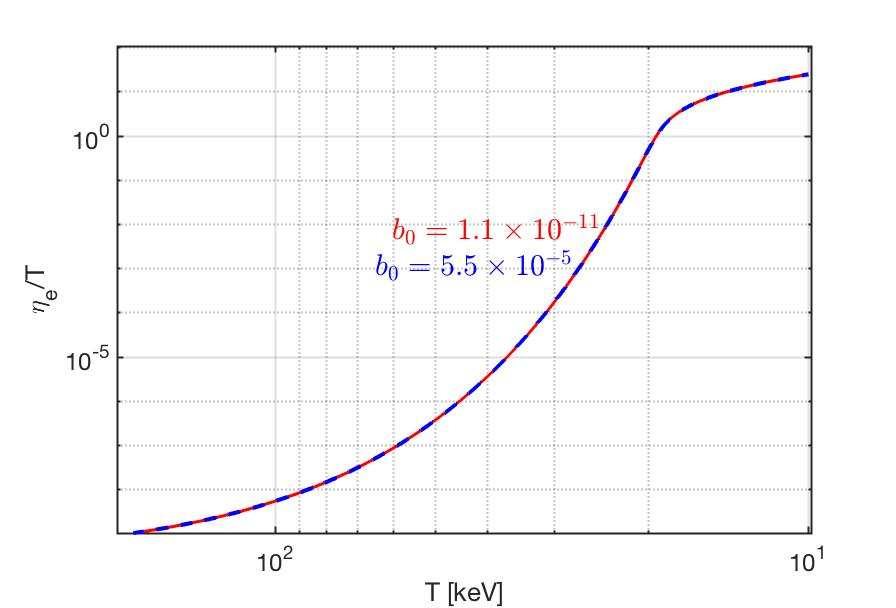
\includegraphics[width=\textwidth]{./plots/ChemicalPotentialFinal_200keV.jpg}
\caption{The chemical potential $\eta_{e}/T$ a function of temperature $10<T<200$keV.  It shows that the chemical potential is not sensitive to the magnetic field $b_0$.}
\label{chemical_fig} 
\end{figure}
%%%%%%%%%%%%%%%%%%%%%%%%%%%%%%%%%%%%%%%
In {\rf{chemical_fig}}, we plot the  chemical potential as a function of temperature $T$. It shows that the chemical potential is not sensitive to the magnetic field because the small value of $b_0=10^{-3}\sim10^{-8}$ and can be neglected in \req{ChemicalPotential}.

%%%%%%%%%%%%%%%%%%%%%%%%%%%%%%%%%%%%%%%
\subsection{Magnetization}\label{sec:Magnetization}
\noindent Given the partition function \req{lnZ} the magnetization can be obtained via the definition
\begin{align}
M=\frac{T}{V}\frac{\partial \ln\mathcal{Z}_{tot}}{\partial B}=\frac{T}{V}\left(\frac{\partial\tilde m_\pm}{\partial B}\right)\frac{\partial \ln\mathcal{Z}_{tot}}{\partial\tilde m_\pm}
\end{align}
then the magnetization can be written as
\begin{align}\label{Magnetization}
    \left(\frac{M}{B}\right)&=\frac{4\pi\alpha}{2\pi^2b_0}\left[2\cosh\left(\frac{\eta_{e}}{T}\right)\right]\sum_{i=\pm}\left\{c_{1}(x_{i})K_1(x_i)+c_{0}K_0(x_i)\right\}\,,\\
    c_{1}(x_{i}) &= \left[\frac{1}{2}-\left(\frac{1}{2}+\frac{ig}{4}\right)\left(1+\frac{b^2_0}{12x^2_i}\right)\right]x_i\,,\qquad c_{0} = \left[\frac{1}{6}-\left(\frac{1}{4}-\frac{ig}{8}\right)\right]b_0\,.
\end{align}
Substituting the chemical potential \req{ChemicalPotential} into \req{Magnetization} we can solve the magnetization $M/B$ numerically.
%%%%%%%%%%%%%%%%%%%%%%%%%%%%%%%%%%%%%%%
\begin{figure}[ht]
%\begin{center}
\centering
%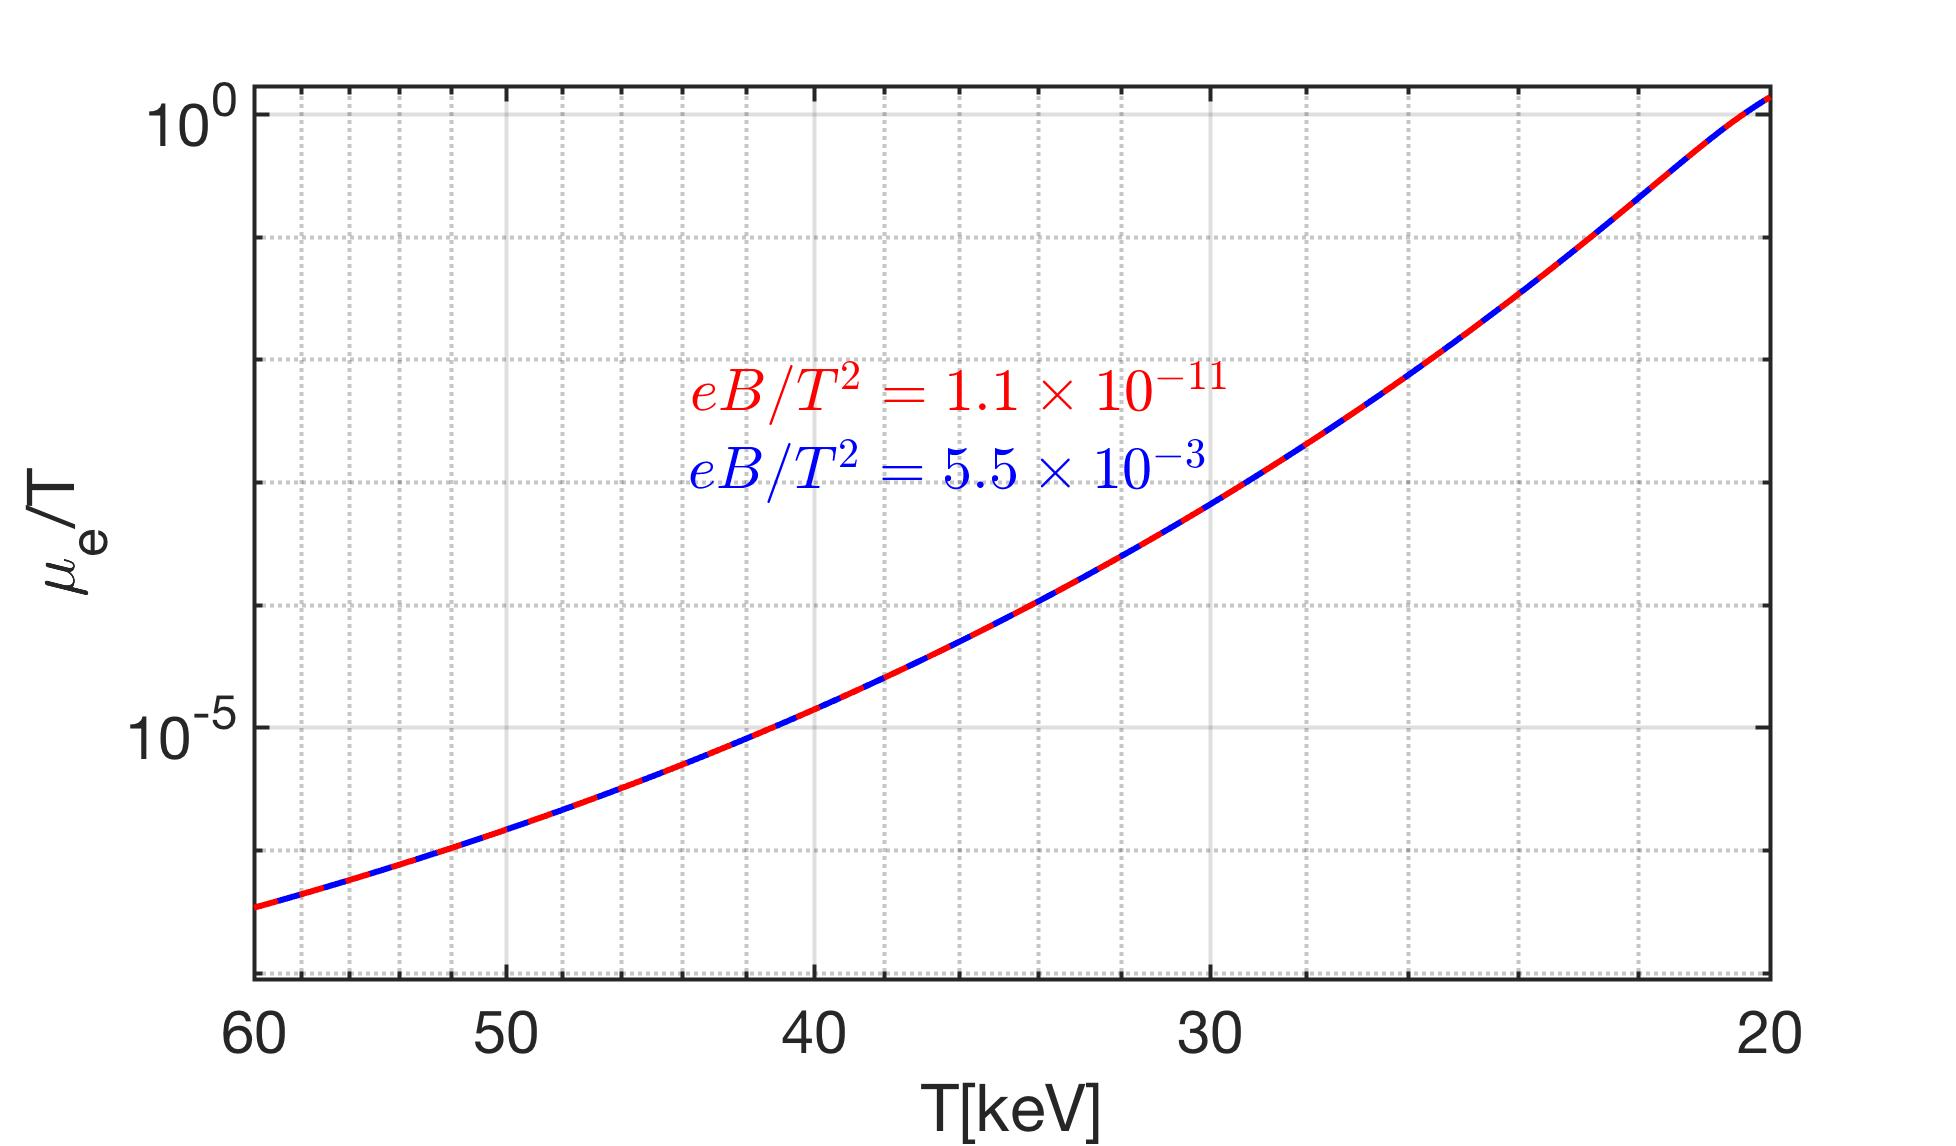
\includegraphics[width=0.75\linewidth]{./plots/ChemicalPotential_case2.jpg}
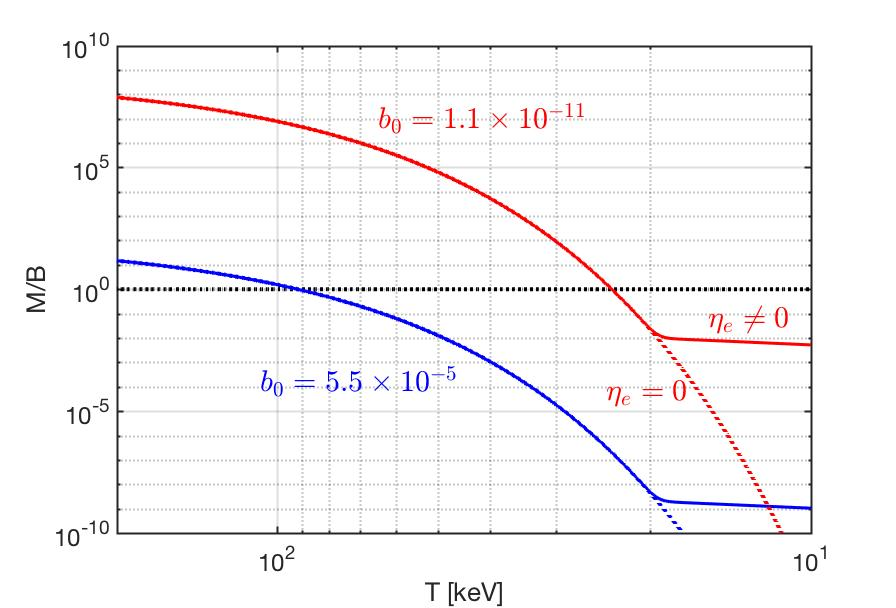
\includegraphics[width=\textwidth]{./plots/MagnetizationFinal_200keV.jpg}
\caption{The magnetization $M/B$ as a function of temperature $10<T<200$ keV, where the solid line represent the case $\mu_e\neq0$ and dotted lines label the case $\mu_e=0$.  It shows that for giving $b_0$ we can find the temperature that $M/B>1$ in early Universe.}
\label{Case2_fig} 
\end{figure}
%%%%%%%%%%%%%%%%%%%%%%%%%%%%%%%%%%%%%%%
Considering the case $g=2$ the magnetization becomes
\begin{align}
\left(\frac{M}{B}\right)=\left(\frac{M}{B}\right)_++\left(\frac{M}{B}\right)_-
\end{align}
where the functions $(M/B)_\pm$ are defined as 
\begin{itemize}
  \item Case1: $\tilde m_+=\sqrt{m^2_e+2eB}$, and $x_+=\tilde m_+/T$. The magnetization is given by
\begin{align}\label{Magnetization_001}
 \left(\frac{M}{B}\right)_+&=-\frac{8\pi\alpha}{2\pi^2}\sqrt{1+\sinh^2(\eta_e/T)}\left[\left(\frac{1}{2b_0}+\frac{b_0}{12x_+^2}\right)x_+K_1(x_+)+\frac{1}{3}K_0(x_+)\right]
\end{align}
Substituting the magnetic field $b_0$ and proton density $n_p/T^3$  we can solve the magnetization and chemical potential numerically. In \rf{Case1_fig}, {\xred Missing figure?} we plot the  magnetization $M/B$ as a function of temperature $T$. It shows for the case1 the magnetization is not sensitive to the magnetic field, this is because the small value of $b_0=10^{-3}\sim10^{-8}$ and can be neglected in \req{chemical_001} {\xred Missing equation?} and \req{Magnetization_001}.
  \item Case 2: $\tilde m_-=m_e$ and $x=\tilde m_-/T$,then the magnetization of electron/ positron becomes
\begin{align}\label{Magnetization_002}
\left(\frac{M}{B}\right)_-&=\frac{8\pi\alpha}{2\pi^2}\sqrt{1+\sinh^2(\eta_e/T)}\left(\frac{1}{b_0}x_-K_1(x_-)+\frac{1}{6}K_0(x_-)\right)
\end{align}
Using the magnetic field $b_0$ and proton density $n_p/T^3$ we solve the magnetization  numerically. In \rf{Case2_fig}, we plot the  magnetization $M/B$ as a function of temperature $T$. It shows that the magnetization depends on the magnetic field $b_0$ strongly. This is because for a small magnetic field $b_0$ the dominant term in \req{Magnetization_002} is $xK_1(x)/b_0$. For given $b_0$, the value of magnetization can be larger than the magnetic field, i.e. $M/B>1$  which shows the possibility that magnetic domains can be formed in the early Universe.
\end{itemize}

%%%%%%%%%%%%%%%%%%%%%%%%%%%%%%%%%%%%%%%
\section{Looking in the Cosmic Rear-view Mirror}\label{Summary}
\noindent The present day Universe seems devoid of antimatter but the primordial Universe was nearly matter-antimatter symmetric. There was only a fractional nano-scale excess of matter which today makes up the visible matter we see around us. All that remains of the tremendous initial amounts of matter-antimatter from the Big Bang is now seen as background entropy. The origin of this nano-asymmetry remains to this day an unresolved puzzle. If asymmetry was created along the path of Universe evolution, as most think, a set of three Sakharov conditions of 1988/91~\cite{Sakharov:1988vdp} (see also the seminal work~\cite{Sakharov:1967dj} of 1967) needs to be fulfilled:
\begin{itemize}
    \item Absence of baryonic charge conservation 
    \item Violation of CP-invariance
    \item Non-stationary conditions in absence of local thermodynamic equilibrium
\end{itemize}
Efforts to create a framework satisfying the above conditions while fitting the observed Universe's evolution so far have failed. One possible solution could be that the standard hypothesis - electroweak phase transition near $T=130\GeV$ - as being the right environment needs considerable amendment. We note that the electroweak transition period (EWT) period is too quick compared to the slower reaction rates given by the known CP-violation in the Standard Model to account for the baryon asymmetry. Additionally is unclear in what fashion the EWT period would contain non-stationary thermodynamics to satisfy the third Sakharov condition. We described (see \rsec{BottomCharm}) that the QGP epoch (a comparably longer time frame of $\approx30\ \mu$secs) possessed bottom quarks in non-equilibrium abundance which should invoke reconsideration of the QGP epoch as possible source for baryon asymmetry \cite{Yang:2020nne,Yang:2023bot}. Our presented work here provides a direction in which we can in the future reconsider this challenge.

We explored several major epochs in the Universe evolution where antimatter, in all its diverse forms, played a large roll. Emphasis was placed on understanding the thermal and chemical equilibria arising within the context of the Standard Model of particle physics. We highlighted that primordial quark-gluon plasma (QGP) is an important antimatter laboratory with its gargantuan antimatter content. Knowledge of the QGP epoch informs our understanding of the fireballs created in heavy-ion collisions performed today and vice versa \cite{Rafelski:2013qeu,Petran:2013lja,Philipsen:2012nu}. The primordial quark-gluon plasma under cosmic expansion however explores a location in the phase diagram of QCD inaccessible to relativistic collider experiments considering both net baryon density and longevity of the plasma.

We described a few interesting results bridging the temperature gap between QGP hadronization at temperature $T\simeq150\MeV$ and  neutrino freezeout:
\begin{itemize}
\item Non-equilibrium abundance of bottom quarks near the QGP hadronization transformation.
\item[] Persistence of:
\item strangeness abundance beyond the loss of the anti-baryons at $T=38.2\MeV$.
\item pions equilibrated via photon production long after the other hadrons disappear.
\item muons disappearing at around $T=4.2\MeV$, the condition when their decay rate outpaces their production rate.
\end{itemize}
At yet lower temperatures neutrinos make up the largest energy fraction in the Universe driving the radiation dominated cosmic expansion. Partway through this neutrino dominated universe, at temperature $T=3.5-1\MeV$ (range from differing flavor freezeout, chemical equilibria, and standard natural constants; see \rf{fig:freezeoutT}), the neutrinos freezeout and decouple from the rest of the thermally active matter in the Universe. We show the neutrino decoupling condition as a function of elementary constants: If these constants were not all ``constant'' a significant entropy flow of annihilating $e^{\pm}$ plasma into neutrinos could be present, generating additional so-called neutrino degrees of freedom.

We study in detail the evolving disappearance of the lightest antimatter, the positrons, and show that positron abundance is large  (see \rf{Density_fig}) during and after Big Bang Nucleosynthesis (BBN). In fact the energy density of electron-positron plasma exceeds greatly that of baryonic matter (see \rf{ratio_fig}) during and following the BBN period with the last positrons vanishing from the Universe near temperature $T=20\keV$. The role of positrons in the eventual large scale structure formation of the Universe has yet to be explored.

Another reason to explore the $e^{\pm}$ epoch, because of its abundance of positrons, is as a parallel for extreme astrophysical systems which produce gamma-ray bursts (GRB). GRBs present an interesting challenge in that a tremendous amount of matter \cite{Aksenov:2010vi} must be converted into light in a short time-span of a few seconds. Ruffini and collaborators \cite{Ruffini:2001fe,Ruffini:2003yt,Ruffini:2009hg,Aksenov:2008zz,Ruffini:2012it,Han:2011er} suggests that  production of large amounts of antimatter which can be subsequently annihilated offers the most direct solution. This avoids the problem of excessive photon pressure, from producing positrons thermally, in GRB producing objects. However, we propose that the production step may  not be required: Some GRB events (especially those which lack classic supernova after-signatures) \cite{Burns:2023oxn,Levan:2023doz} may originate from novel stellar objects which naturally possess, rather than create, larger amounts of antimatter (positrons) capable of rapid catalysis of gamma-rays upon gravitational collapse. Such novel stellar objects could have internal conditions not unlike the primordial plasmas of the early Universe. We are hoping to look into this in the near future, also in the context of strongly magnetized objects (magnetars).

Looking forward, we note that some of the topics we explored deserve a more intense followup work: 
\begin{itemize}
    \item The study of matter baryogenesis in the context of bottom quarks which persists, in chemical non-equilibrium, to the late QGP evolution.
    \item The impact of relatively dense $e^{\pm}$ plasma on BBN processes.
    \item Exploration of spatial inhomogeneities in dense $e^{\pm}$ plasma driven by spontaneous self magnetization.
    \item The search for GRB capable objects with positron content including super-heavy hot stars with core temperatures in excess of $T>20\keV$.
\end{itemize}

Looking into the rear-view mirror of the cosmos, our work within the realm of the Standard Model of particle and plasma physics bridges the early universe of QGP and on-wards to the still unsolved pre-QGP early universe as explored in the seminal work by Fang and Ruffini.

We hope that this work provides to all interested parties a first glimpse at the long ignored but very interesting epoch of Universe evolution involving in sequence numerous plasma phases made of all particles known today. 
%%%%%%%%%%%%%%%%%%%%%%%%%%%%%%%%%%%%%%%
\begin{figure}[H]
%\begin{center}
\centering

\includegraphics[width=\textwidth]{./plots/remo_sunset}
\caption{Remo Ruffini and Johann Rafelski beneath a sunset in Tucson, AZ on October 7th, 2012. The photo taken by She Sheng Xue was at a celebratory gathering honoring the life of Fang Li-Zhi.}
\label{remo_sunset}
\end{figure}
%%%%%%%%%%%%%%%%%%%%%%%%%%%%%%%%%%%%%%%
%%%%%%%%%%%%%%%%%%%%%%%%%%%%%%%%%%%%%%%
\reftitle{References}
%\bibliographystyle{ieeetr}
\bibliography{refs}
%%%%%%%%%%%%%%%%%%%%%%%%%%%%%%%%%%%%%%%
\end{document}
